\documentclass[11pt]{article}
\usepackage[T1]{fontenc}
\usepackage{amssymb}
\usepackage{amsmath}
\usepackage{amsthm}
\usepackage{bm}
\usepackage{graphicx}
\usepackage{dsfont}
\usepackage[makeroom]{cancel}
\usepackage{mathtools}
\usepackage{commath}
\usepackage[english]{babel}
\usepackage[utf8]{inputenc}
\usepackage{fancyhdr}
\usepackage{bold-extra}
\usepackage{color}   
\usepackage{hyperref}
\usepackage{tocloft}
\usepackage[shortlabels]{enumitem}
\usepackage{pgfplots}
\usepgfplotslibrary{fillbetween}
\usetikzlibrary{patterns}

\theoremstyle{definition}
\newtheorem{thm}{Theorem}[section]

\newtheorem{defn}[thm]{Definition}
\newtheorem{exmp}[thm]{Example}
\newtheorem{prop}[thm]{Proposition}
\newtheorem{cor}[thm]{Corollary}
\newtheorem{lemma}[thm]{Lemma}
\newtheorem{remark}[thm]{Remark}
\newtheorem{notation}[thm]{Notation}
\newtheorem{exercise}[thm]{Exercise}
\newtheorem{app}[thm]{Applications}
\newtheorem{none}[thm]{}
\newtheorem{caveat}[thm]{Caveat}

\newcommand{\mbN}{\ensuremath{\mathbb{N}}}
\newcommand{\mbZ}{\ensuremath{\mathbb{Z}}}
\newcommand{\mbQ}{\ensuremath{\mathbb{Q}}}
\newcommand{\mbR}{\ensuremath{\mathbb{R}}}
\newcommand{\mbC}{\ensuremath{\mathbb{C}}}

% L'Hopital's Rule
\newcommand{\lhr}{\stackrel{\mathclap{\mbox{\normalfont\tiny L'HR}}}{=}}

% Pointwise/Uniform Convergence
\newcommand{\ptwise}{\xrightarrow{\text{pointwise}}}
\newcommand{\unif}{\xrightarrow{\text{uniformly}}}

% Power Series
\newcommand{\powerseries}{\ensuremath{S(x) = \sum_{k=0}^\infty a_k (x - x_0)^k \text{ }}}

% 1-inch margins
\topmargin 0pt
\advance \topmargin by -\headheight
\advance \topmargin by -\headsep
\textheight 8.9in
\oddsidemargin 0pt
\evensidemargin \oddsidemargin
\marginparwidth 0.5in
\textwidth 6.5in

\parindent 0in
\parskip 1.5ex

% hyperlinks
\hypersetup{
  colorlinks=true, 
  linktoc=all,     % table of contents is clickable  
  allcolors=blue   % all hyperlink colours
}

% table of contents
\addto\captionsenglish{
  \renewcommand{\contentsname}%
    {Table of Contents}%
}

% headers and footers
\pagestyle{fancy}
\renewcommand{\sectionmark}[1]{\markboth{#1}{#1}}
%\lhead{Winter 2019}
\lhead{MATH 148: Calculus 2 (Advanced Level)}
\fancyhead[R]{Chapter \thesection: \em \leftmark}
\cfoot{\thepage}
\setlength\headheight{14pt}

% title and preface formatting
\newcommand{\newtitle}[4]{
  \begin{center}
	\huge{\textbf{\textsc{#1 Course Notes}}}
    
	\large{\sc #2}
    
	{\sc #3 \textbullet\, #4 \textbullet\, University of Waterloo}
	\normalsize\vspace{1cm}\hrule\vspace{0.5cm}
	
	\textbf{Preface}
  \end{center}
  \vspace{-0.4cm}
  These notes were created as a resource for personal use, and for current, past, and future students of the course. They may contain errors and inconsistencies. If you notice any errors or have other inquiries regarding these notes, feel free to e-mail me at {\tt mltlee@uwaterloo.ca}. \vspace{1cm}\hrule\vspace{0.5cm}
}

\setcounter{section}{-1}

\pgfplotsset{compat=1.15}

\begin{document}

% title and preface
\newtitle{MATH 148}{Calculus 2 (Advanced Level)}{Laurent Marcoux}{Winter 2019}

\tableofcontents\thispagestyle{fancy}
\rhead{\em Table of Contents}
\vspace{1cm}\hrule
\newpage
\fancyhead[R]{Chapter \thesection: \em \leftmark}

% Chapter 0
\section{Motivating the Riemann Integration}

% 0.1
\begin{none} 
The concept of Riemann integration has many applications. We study two such applications to motivate the definition.
\end{none}

% 0.2
\begin{exmp}
Consider a person who is walking for 2 hours, equipped with a watch and a speedometer (which measures speed but not distance). The problem is to determine the total distance walked over the 2 hour period. 

We attack this problem by partitioning the time interval from $t = 0$ to $t = 2$ into smaller intervals.
$$0 = t_0 < t_1 < \dots < t_N = 2$$
Let $V_i$ be the maximum speed over the time interval $[t_{i-1}, t_i]$, and $v_i$ be the minimum speed over $[t_{i-1}, t_i]$, where $1 \leq i \leq N$. 

If $d_i$ is the distance covered in the time interval $[t_{i-1}, t_i]$, $1 \leq i \leq N$, then 
$$v_i (t_i - t_{i-1}) \leq d_i \leq V_i (t_i - t_{i-1})$$
Thus the total distance covered satisfies
$$\sum_{i=1}^N v_i (t_i - t_{i-1}) \leq d = \sum_{i=1}^N d_i \leq \sum_{i=1}^N V_i (t_i - t_{i-1})$$
given that the speed of a person walking is a continuous function of time (by hypothesis), and we know that the speed function is uniformly continuous on $[0, 2]$.

Thus, given $\varepsilon > 0$, we can find $\delta > 0$ such that if $\max_{1 \leq i \leq N} t_i - t_{i-1} < \delta$, then $\max_{1 \leq i \leq N} V_i - v_i < \varepsilon$, in which case
\begin{align*}
\left(\sum_{i=1}^N V_i (t_i - t_{i-1})\right) - \left(\sum_{i=1}^N v_i (t_i - t_{i-1})\right) 
& = \sum_{i=1}^N (V_i - v_i)(t_i - t_{i-1}) \\
& \leq \sum_{i=1}^N \varepsilon(t_i - t_{i-1}) \\
& = \varepsilon \sum_{i=1}^N (t_i - t_{i-1}) \\
& = \varepsilon \Big( (t_N - \cancel{t_{N-1}}) + (\cancel{t_{N-1}} - \cancel{t_{N-2}}) + \dots + (\cancel{t_1} - t_0)\Big) \\
& = \varepsilon(t_N - t_0) = \varepsilon(2 - 0) = 2\varepsilon
\end{align*}
Thus we can estimate $d$ to within $2\varepsilon$ using this argument.
\end{exmp}

% 0.3
\begin{exmp}
Suppose $f : [0, 2] \to [0, \infty)$ is continuous. We wish to calculate the area $A$ under the curve $y = f(x)$ from $x = 0$ to $x = 2$. 

% \includegraphics[width=\linewidth]{images/1.jpg}
As before, we partition the interval $[0, 2]$ as follows: 

We set 
$$0 = t_0 < t_1 < \dots < t_N = 2$$
and let $M_i = \max_{x \in [t_{i-1}, t_i]} f(x)$ and $m_i = \min_{x \in [t_{i-1}, t_i]} f(x)$, where $1 \leq i \leq N$, which exist because $f$ is continuous on $[t_{i-1}, t_i]$, $1 \leq i \leq N$. 

Then we see that
$$\sum_{i=1}^N m_i (t_i - t_{i-1}) \leq A \leq \sum_{i=1}^N M_i (t_i - t_{i-1})$$
Arguing as in Example 0.2, since $f$ is continuous on $[0, 2]$, it is uniformly continuous on $[0, 2]$, so given $\varepsilon > 0$, there exists $\delta > 0$ such that
$$\max_{1 \leq i \leq N} t_i - t_{i-1} < \delta \implies \max_{1 \leq i \leq N} M_i - m_i < \varepsilon$$
hence $A$ can be approximated to within $2\varepsilon$ by either $\sum_{i=1}^N m_i(t_i - t_{i-1})$ or $\sum_{i=1}^N M_i(t_i - t_{i-1})$.
\end{exmp}

\newpage

% Chapter 1
\section{An Introduction to Riemann Integration}

% 1.1
\begin{notation}
Throughout this course, we shall use the following notation: \vspace{-0.2cm}
\begin{itemize}
\item $[a, b] = \{x \in \mbR : a \leq x \leq b\}$; it is assumed that $a \leq b \in \mbR$.
\item We denote an arbitrary (not necessarily bounded or closed) interval by $\mathds{I}$.
\end{itemize}
\end{notation}

% 1.2
\begin{defn}
Let $[a, b] \subseteq \mbR$ be an interval. 

A \textbf{partition} of $[a, b]$ is a finite set of the form 
$$P = \{a = p_0 < p_1 < \dots < p_N = b\}$$
The \textbf{norm} of a partition $P$ is
$$\norm{x} = \max_{1 \leq i \leq N} p_i - p_{i-1}$$
% \includegraphics[width=\linewidth]{images/2.jpg}
We say that a partition $P$ is \textbf{uniform} if $p_i - p_{i-1} = \frac{b-a}N$ with $1 \leq i \leq N$. 

Equivalently, $P$ is uniform if $\norm{P} = \frac{b-a}N$.

We set $\mathcal{P}[a, b] = \{P : P \text{ is a partition of } [a, b]\}$.
\end{defn}

% 1.3
\begin{notation}
Let $f : [a, b] \to \mbR$ be a \textbf{bounded} function. 

Let $P \in \mathcal{P}[a, b]$, say $P = \{a = p_0 < p_1 < \dots < p_N = b\}$. 

We define
$$ M_i (= M_i (f, P)) = \sup_{x \in [p_{i-1}, p_i]} f(x) $$
$$ m_i (= m_i (f, P)) = \inf_{x \in [p_{i-1}, p_i]} f(x) $$
where $1 \leq i \leq N$. 

\textbf{Note:} $M_i$ and $m_i$ depend on the choice of $f$ and $P$.
\end{notation}

% 1.4
\begin{exmp} 
Some applications: \vspace{-0.2cm}
\begin{enumerate}[(a)]

\item Let $f : [a, b] \to \mbR$. 
$$ f(x) = \begin{cases}
			1 & x \in \mbQ \cap [a, b] \\
			0 & x \in [a, b] \setminus \mbQ
		 \end{cases} $$
If $P \in \mathcal{P}[a, b]$, say $P = \{a = p_0 < p_1 < \hdots < p_N = b\}$, then $M_i = 1$ and $m_i = 0$, with $1 \leq i \leq N$.

\item Suppose that $f : [a, b] \to \mbR$ is \underline{decreasing} (i.e. $a \leq x \leq y \leq b \implies f(x) \geq f(y)$). 

If $P = \{a = p_0 < p_1 < \hdots < p_N = b\} \in \mathcal{P}[a, b]$, then $M_i = f(p_{i-1})$ and $m_i = f(p_i)$, $1 \leq i \leq N$.

\end{enumerate}
\end{exmp}

% 1.5
\begin{defn}
We define the \textbf{lower Riemann sum} to be
$$L(f, P) = \sum_{k=1}^N m_k (p_k - p_{k-1}) $$
and the \textbf{upper Riemann sum} to be
$$U(f, P) = \sum_{k=1}^N M_k (p_k - p_{k-1}) \text{.}$$
Note that $m_k \leq M_k$, and $p_k - p_{k-1} > 0$, $1 \leq k \leq N$, which implies that
$$L(f, P) \leq U(f, P) \text{.}$$
\end{defn}

% 1.6
\begin{exmp}~ \vspace{-0.2cm}

\begin{enumerate}[(a)]

\item Consider the function $f : [0, 1] \to \mbR$.
$$ f(x) = \begin{cases}
			\frac12x & x \in [0, \frac12) \\
			0 & x = \frac12 \\
			\frac12x - \frac12 & x \in (\frac12, 1]
             \end{cases} $$
% \includegraphics[width=\linewidth]{images/3.jpg}
Consider the partition
$$P = \{0, 1/3, 2/3, 1\} \text{.}$$
Then,
\begin{align*}
m_1 & = 0 & m_2 & = -1/4 & m_3 & = -1/6 \\
M_1 & = 1/6 & M_2 & = 1/4 & M_3 & = 0
\end{align*}
so that
\begin{align*}
L(f, P) & = m_1 \left(1/3 - 0\right) + m_2 \left(2/3 - 1/3\right) + m_3 \left(1 - 2/3\right) \\
	   & = 0 \left(1/3\right) + \left(-1/4\right)\left(1/3\right) + \left(-1/6\right)\left(1/3\right) \\
	   & = -1/12 - 1/18 = -5/36 \\
U(f, P) & = M_1 \left(1/3 - 0\right) + M_2 \left(2/3 - 1/3\right) + M_3 \left(1 - 2/3\right) \\
	    & = (1/6) \left(1/3\right) + (1/4) \left(1/3\right) + 0\left(1/3\right) \\
	    & = 5/36
\end{align*}

\item Let $f : [a, b] \to \mbR$.
$$x \mapsto \begin{cases}
				1 & x \in \mbQ \cap [a, b] \\
				0 & x \in [a, b] \setminus \mbQ
			\end{cases} $$
Let $P = \{a = p_0 < p_1 < \hdots < p_N = b\} \in \mathcal{P}[a, b]$. 
Then $m_k = 0$, $M_k = 1$, $1 \leq k \leq N$. Thus,
\begin{align*}
L(f, P) & = \sum_{k=1}^N m_k (p_k - p_{k-1}) = \sum_{k=1}^N 0(p_k - p_{k-1}) = 0 \\
U(f, P) & = \sum_{k=1}^N M_k (p_k - p_{k-1}) = \sum_{k=1}^N 1 (p_k - p_{k-1}) \\
	    & = (p_1 - p_0) + (p_2 - p_1) + \hdots + (p_N - p_{N-1}) \\
	    & = p_N - p_0 \\
	    & = b - a
\end{align*}
\textbf{Note:} These are independent of the choice of $P$. 

\item Consider 
\begin{align*}
f : [0, 1] & \to \mbR \\
	   x & \mapsto x^2
\end{align*}
Let $P = \{0 < \frac1N < \frac2N < \hdots < \frac{N-1}N < 1 = p_N\}$ (i.e. $p_k = \frac{k}N, 0 \leq k \leq N$) be a uniform partition. 

Since $f$ is increasing on $[0, 1]$,
\begin{align*}
m_k & = f(p_{k-1}) = f\left(\frac{k-1}N\right) = \left(\frac{k-1}N\right)^2 \\
M_k & = f(p_k) = f\left(\frac{k}N\right) = \left(\frac{k}N\right)^2
\end{align*}
Hence, we have
\begin{align*}
U(f, P) & = \sum_{k=1}^N M_k (p_k - p_{k-1}) & L(f, P) & = \sum_{k=1}^N m_k (p_k - p_{k-1}) \\
& = \sum_{k=1}^N \left(\frac{k}N\right)^2 \left(\frac1N\right) & & = \sum_{k=1}^N \left(\frac{k-1}N\right)^2 \left(\frac1N\right) \\
& = \frac1{N^3} \sum_{k=1}^N k^2 & & = \frac1{N^3} \sum_{k=1}^N (k-1)^2 \\
& = \frac1{N^3} \left(\frac{N(N+1)(2N+1)}6\right) & & = \frac1{N^3} \sum_{k=0}^{N-1} k^2 \\
& = \frac{1(1+\frac1N)(2+\frac1N)}6 & & = \frac1{N^3} \sum_{k=1}^{N-1} k^2 \\
& & & = \frac1{N^3} \left(\frac{(N-1)(N)(2N-1)}6\right) \\
& & & = \frac{(1-\frac1N)(1)(2-\frac1N)}6
\end{align*}
It follows that
$$\lim_{N\to\infty} L(f, P = P_N) = \frac13 = \lim_{N\to\infty} U(f, P = P_N) \text{.}$$

\end{enumerate}
\end{exmp}

% 1.7
\begin{defn}
Let $[a, b] \in \mbR$ and $P \in \mathcal{P}[a, b]$. 

We say that $Q \in \mathcal{P}[a, b]$ is a \textbf{refinement} of $P$, or that $Q$ \textbf{refines} $P$, if $P \subseteq Q$. 
\end{defn}

% 1.8
\begin{exmp}
Consider $P = \{0, \frac14, \frac12, \frac9{10}, 1\} \in \mathcal{P}[0, 1]$. 

Let
\begin{align*}
Q_1 & = \left\{0, \frac14, \frac13, \frac12, \frac34, \frac9{10}, 1 - \frac{\pi}{10^{23}}, 1\right\} \\
Q_2 & = \left\{0, \frac19, \frac29, \hdots, \frac89, 1\right\} \\
Q_3 & = \left\{0, \frac14, \frac12, \frac9{10}, 1, \frac32\right\}
\end{align*}
$Q_1$ is a refinement of $P$. 

$Q_2$ is \textbf{not} a refinement of $P$ since $\frac14 \in P$ but $\frac14 \notin Q_2$. 

$Q_3$ is \textbf{not} a refinement of $P$ since $Q_3 \notin \mathcal{P}[0, 1]$.
\end{exmp}

% 1.9
\begin{prop}
Let $f : [a, b] \to \mbR$ be a bounded function, and let $P \in \mathcal{P}[a, b]$. If $Q$ is a refinement of $P$, then
$$L(f, P) \leq L(f, Q) \leq U(f, Q) \leq U(f, P) \text{.}$$
\end{prop}
\textbf{Proof.}

\textbf{Case 1.} $Q$ has exactly 1 more point than $P$.

Consider $P = \{a = p_0 < p_1 < ... < p_N = b\}$ and $Q = P \cup \{r\}$, where $p_{k-1} < r < p_k$ for some fixed $1 \leq k \leq N$. 

Let $m_j = \inf \{f(x) : x \in [p_{j-1}, p_j]\}, 1 \leq j \leq N$. 

We define the following:
\begin{align*}
{m_k}' & := \inf \{f(x) : x \in [p_{k-1}, r]\} \\
{m_k}'' & := \inf \{f(x) : x \in [r, p_k]\}
\end{align*}
Then
\begin{align*}
L(f, P) & = \sum_{j=1}^N m_j (p_j - p_{j-1})
\intertext{while}
L(f, Q) & = \sum_{j=1}^{k-1} m_j (p_j - p_{j-1}) + {m_k}' (r - p_{k-1}) + {m_k}'' (p_k - r) + \sum_{j=k+1}^N m_j (p_j - p_{j-1})
\intertext{and so}
L(f, Q) - L(f, P) & = {m_k}' (r-p_{k-1}) + {m_k}'' (p_k - r) - m_k \Big( (p_k - r) + (r - p_{k-1}) \Big) \\
			   & = ({m_k}' - m_k)(r - p_{k-1}) + ({m_k}'' - m_k)(p_k - r)
\end{align*}
Since ${m_k}' \geq m_k$ and ${m_k}'' \geq m_k$, all of the above terms are greater than or equal to 0, which implies that
$$L(f, Q) - L(f, P) \geq 0 \implies L(f, P) \leq L(f, Q) \text{.}$$
\textbf{Exercise:} Prove that $U(f, Q) \leq U(f, P)$. 

Hence, $L(f, P) \leq L(f, Q) \leq U(f, Q) \leq U(f, P)$. 

\textbf{Case 2.} The general case. 

Suppose $Q = P \cup \{r_1, r_2, \hdots, r_m\}$. 

Set $Q_0 = P$, and for $1 \leq j \leq m$, set $Q_j = Q_{j-1} \cup \{r_j\}$. 

Then, by Case 1, noting that each $Q_j$ is a refinement of $Q_{j-1}$ with exactly 1 more point, we find that
\begin{align*}
L(f, P) = L(f, Q_0) & \leq L(f, Q_1) \\
				 & \leq L(f, Q_2) \\
				 & \leq \hdots \\
				 & \leq L(f, Q_m) \\
				 & = L(f, Q) \\
				 & \leq U(f, Q) \\
				 & = U(f, Q_m) \\
				 & \leq U(f, Q_{m-1}) \\
				 & \leq \hdots \\
				 & \leq U(f, Q_0) = U(f, P) \hspace{5pt} \qedsymbol
\end{align*}

% 1.10
\begin{cor}
Let $f : [a, b] \to \mbR$ be a bounded function. 

If $P, Q \in \mathcal{P}[a, b]$, then 
$$L(f, P) \leq U(f, Q) \text{.}$$
\end{cor}
\textbf{Proof.}
Let $R = P \cup Q \in \mathcal{P}[a, b]$, so $R$ is a \underline{common} refinement of $P$ and $Q$. 

By Proposition 1.9, we have that
$$L(f, P) \leq L(f, R) \leq U(f, R) \leq U(f, Q) \text{.} \hspace{5pt} \qedsymbol$$

% 1.11
\begin{defn}
Let $f : [a, b] \to \mbR$ be a bounded function. 

We define the \textbf{lower Riemann integral} of $f$ over $[a, b]$ to
$$L\int_a^b f := \sup\{L(f, P) : P \in \mathcal{P}[a, b]\} < \infty \text{.}$$
Similarly, we define the \textbf{upper Riemann integral} of $f$ over $[a, b]$ to be
$$U\int_a^b f := \inf\{U(f, Q) : Q \in \mathcal{P}[a, b]\} \in \mbR \text{.}$$
We observe that
$$L\int_a^b f \leq U\int_a^b f \text{.}$$
To see this, note that if we fix $Q \in \mathcal{P}[a, b]$, then
$$L(f, P) \leq U(f, Q) \hspace{10pt} \forall P \in \mathcal{P}[a, b]$$
implies that
$$L\int_a^b f = \sup\{L(f, P) : P \in \mathcal{P}[a, b]\} \leq U(f, Q) \text{.}$$
That is,
$$L\int_a^b f \leq U(f, Q) \text{.}$$
But this holds for all $Q \in \mathcal{P}[a, b]$, whence
$$L\int_a^b f \leq \inf\{U(f, Q) : Q \in \mathcal{P}[a, b]\} = U\int_a^b f \text{.}$$
\end{defn}

% 1.12
\begin{exmp}~ \vspace{-0.2cm}
\begin{enumerate}[(a)]

\item Consider
\begin{align*}
f : [a, b] & \to \mbR \\
          x & \mapsto \begin{cases}
          				1 & x \in \mbQ \cap [a, b] \\
          				0 & x \in [a, b] \setminus \mbQ
				   \end{cases}
\end{align*}
We saw in Example 1.6 that
\begin{align*}
L(f, P) & = 0 \\
U(f, P) & = b - a
\end{align*}
for all $P \in \mathcal{P}[a, b]$. Hence,
\begin{align*}
L\int_a^b f & = \sup\{0 : P \in \mathcal{P}[a, b]\} = 0 \\
U\int_a^b f & = \inf\{b-a : P \in \mathcal{P}[a, b]\} = b-a
\end{align*}

\item Consider
\begin{align*}
f : [0, 1] & \to \mbR \\
	    x & \mapsto x^2
\end{align*}
Recall from Example 1.6 that if for each $N \geq 1$, we set
$$P_N = \left\{0 < \frac1N < \frac2N < \hdots < \frac{N-1}N < 1 \right\} \in \mathcal{P}[0, 1]$$
then
\begin{align*}
L(f, P_N) & = \frac16\left(1 - \frac1N\right)\left(2 - \frac1N\right) \\
U(f, P_N) & = \frac16\left(1 + \frac1N\right)\left(2 + \frac1N\right)
\end{align*}
Thus,
\begin{align*}
L\int_0^1 f & = \sup\{L(f, P) : P \in \mathcal{P}[0, 1]\} \\
		    & \geq \sup\{L(f, P_N) : N \geq 1\} \\
		    & = \sup\left\{\frac16\left(1-\frac1N\right)\left(2-\frac1N\right) : N \geq 1\right\} = \frac13 \\
\intertext{while}
U\int_0^1 f & = \inf\{U(f, P) : P \in \mathcal{P}[0, 1]\} \\
		     & \leq \inf\{U(f, P_N) : N \geq 1\} \\
		     & = \inf\left\{\frac16\left(1+\frac1N\right)\left(2+\frac1N\right) : N \geq 1\right\} = \frac13 
\end{align*}
It follows that
$$\frac13 \leq L\int_0^1 f \leq U\int_0^1 f \leq \frac13$$
so that
$$L\int_0^1 f = U\int_0^1 f = \frac13 \text{.}$$

\end{enumerate}
\end{exmp}

% 1.13
\begin{defn}
Let $f : [a, b] \to \mbR$ be a bounded function. 

We say $f$ is \textbf{Riemann integrable} over $[a, b]$ if
$$L\int_a^b f = U\int_a^b f$$
in which case we denote the common value by
$$\int_a^b f \text{.}$$
We also write
$$\mathcal{R}[a, b] = \{f : [a, b] \to \mbR \mid f \text{ is Riemann integrable}\} \text{.}$$
\end{defn}

% 1.14
\begin{exmp}~ \vspace{-0.2cm}
\begin{enumerate}[(a)]

\item Consider 
\begin{align*}
f : [a, b] & \to \mbR \\
          x & \mapsto \begin{cases}
          				1 & x \in \mbQ \cap [a, b] \\
          				0 & x \in [a, b] \setminus \mbQ
				   \end{cases}
\end{align*}
with $a < b$ (because this would otherwise be uninteresting). 

From Example 1.12,
$$L\int_a^b f = 0 \neq b - a = U\int_a^b f \text{.}$$
Thus $f$ is \textbf{not} Riemann integrable over $[a, b]$.

\item Let $f(x) = x^2$, $x \in [0, 1]$. Then
$$L\int_0^1 f = U\int_0^1 f = \frac13$$
by Example 1.12, so $f \in \mathcal{R}[0, 1]$, and $\int_0^1 f = \frac13$.

\end{enumerate}
\end{exmp}

% 1.15
\begin{none}
Classifying all Riemann integrable functions is beyond the scope of the course. Instead, we show that $\mathcal{R}[a, b]$ contains a large class of functions, and we develop techniques to evaluate $\int_a^b f$ when possible.
\end{none}

% 1.16
\begin{thm}[The Cauchy Criterion]
Let $f : [a, b] \to \mbR$ be a bounded function. Then the following are equivalent: \vspace{-0.2cm}
\begin{enumerate}[(a)]
\item $f$ is Riemann integrable over $[a, b]$. 
\item For every $\varepsilon > 0$, there exists a partition $P \in \mathcal{P}[a, b]$ such that
$$U(f, P) - L(f, P) < \varepsilon \text{.}$$
\end{enumerate}
\end{thm}

\textbf{Proof.} (a) $\implies$ (b). Suppose that $f \in \mathcal{R}[a, b]$, that is, $L\int_a^b f = U\int_a^b f$. 

Let $\varepsilon > 0$. 

Since $L\int_a^b f = \sup\{L(f, Q) : Q \in \mathcal{P}[a, b]\}$, we can find $Q \in \mathcal{P}[a, b]$ such that
$$L\int_a^b f - L(f, Q) < \frac{\varepsilon}2 \text{.}$$
Similarly, since $U\int_a^b f = \inf\{U(f, R) : R \in \mathcal{P}[a, b]\}$, we can find $R \in \mathcal{P}[a, b]$ such that
$$U(f, R) - U\int_a^b f < \frac{\varepsilon}2 \text{.}$$
% \begin{center} \includegraphics[width=0.8\linewidth]{images/5.jpg} \end{center}
Thus 
\begin{align*}
U(f, R) - L(f, Q) & \leq U(f, R) - U\int_a^b f + L\int_a^b f - L(f, Q) \\
		  	    & < \frac{\varepsilon}2 + \frac{\varepsilon}2 = \varepsilon
\end{align*}
Let $P = Q \cup R \in \mathcal{P}[a, b]$ so that $P$ is a common refinement of $Q$ and $R$. Thus,
\begin{align*}
L(f, Q) \leq L(f, P) & \leq L\int_a^b f \\
				 & = U\int_a^b f \leq U(f, P) \leq U(f, R)
\end{align*}
and
\begin{align*}
U(f, P) - L(f, P) & \leq U(f, R) - L(f, Q) \\
			   & < \varepsilon
\end{align*}
which is what we wanted to show. 

(b) $\implies$ (a). Suppose for every $\varepsilon > 0$, there exists a partition $P \in \mathcal{P}[a, b]$ such that $U(f, P) - L(f, P) < \varepsilon$. 

For each $N \geq 1$, we can choose $P_N \in \mathcal{P}[a, b]$ such that
$$U(f, P_N) - L(f, P_N) < \frac1N \text{.}$$
Recall that
$$L(f, P_N) \leq L\int_a^b f - U\int_a^b f \leq U(f, P_N) \hspace{10pt} \forall N \geq 1$$
and so
\begin{align*}
0 \leq U\int_a^b f - L\int_a^b f & \leq U(f, P_N) - L(f, P_N) \\
							 & < \frac1N, N \geq 1
\end{align*}
Hence
$$U\int_a^b f - L\int_a^b f = 0 \text{,}$$
that is,
$$L\int_a^b f = U\int_a^b f \text{,}$$
so $f \in \mathcal{R}[a, b]$. $\qedsymbol$

% 1.17
\begin{exmp} 
Suppose $a < c < b$ in $\mbR$ and that $0 < r \in \mbR$. 

Consider the function
\begin{align*}
f : [a, b] & \to \mbR \\
          x & \mapsto \begin{cases}
          				0 & x \in [a, c) \\
          				2r & x = c \\
          				r & x \in (a, b]
				   \end{cases}
\end{align*}
% \begin{center} \includegraphics[width=0.8\linewidth]{images/6.jpg} \end{center}
We shall use Cauchy's Criterion to prove that $f \in \mathcal{R}[a, b]$. 

\textbf{Proof.} Let $\varepsilon > 0$. 

Let $\delta = \min\left\{\frac{c-a}2, \frac{b-c}2, \frac{\varepsilon}{4r}\right\}$. 

Consider the partition $P_{\delta} = \{a, c - \delta, c + \delta, b\}$. 

Then we have
\begin{align*}
m_1 & = 0 & M_1 & = 0 \\
m_2 & = 0 & M_2 & = 2r \\
m_3 & = r & M_3 & = r
\end{align*}
Thus, we obtain
\begin{align*}
L(f, P_{\delta}) & = m_1 \Big((c-\delta) - a\Big) + m_2 \Big((c+\delta) - (c - \delta)\Big) + m_3 \Big(b - (c + \delta)\Big) \\
			    & = 0 + 0 + r\Big(b - (c + \delta)\Big) \\
U(f, P_{\delta}) & = M_1 \Big((c-\delta) - a\Big) + M_2 \Big((c+\delta) - (c - \delta)\Big) + M_3 \Big(b - (c + \delta)\Big) \\
			    & = 2r(2\delta) + r\Big(b - (c+\delta)\Big)
\end{align*}
Therefore,
$$U(f, P_{\delta}) - L(f, P_{\delta}) = 2r(2\delta) = \delta(4r) < \varepsilon \text{.}$$
Then by the Cauchy Criterion, $f \in \mathcal{R}[a, b]$. $\qedsymbol$
\end{exmp}

% 1.18
\begin{thm}
Let $a < b \in \mbR$ and suppose that $f : [a, b] \to \mbR$ is an \underline{increasing} function. Then $f \in \mathcal{R}[a, b]$.
\end{thm}
\textbf{Proof.} 
We will use the Cauchy Criterion to prove this. 

Let $\varepsilon > 0$. Let $P \in \mathcal{P}[a, b]$, say
$$P = \{a = p_0 < p_1 < \dots < p_N\}$$
with $\norm{P} := \max_{1 \leq k \leq N} p_k - p_{k-1} < \frac{\varepsilon}{\left(f(b) - f(a)\right) + 1}$. 

Let
\begin{align*}
m_k & = \inf\{f(x) : x \in [p_{k-1}, p_k]\} = f(p_{k-1}) \\
M_k & = \sup\{f(x) : x \in [p_{k-1}, p_k\} = f(p_k)
\end{align*}
$1 \leq k \leq N$. 

Thus,
\begin{align*}
U(f, P) - L(f, P) & = \sum_{k=1}^N M_k (p_k - p_{k-1}) - \sum_{k-1}^N m_k (p_k - p_{k-1}) \\
			   & = \sum_{k=1}^N (M_k - m_k) (p_k - p_{k-1}) \\
			   & \leq \sum_{k=1}^N (M_k - m_k) \norm{P} \\
			   & = \norm{P} \sum_{k=1}^N \Big(f(p_k) - f(p_{k-1})\Big) \\
			   & = \norm{P} \Big(f(p_N) - f(p_0)\Big) \\
			   & = \norm{P} \Big(f(b) - f(a)\Big) \\
			   & < \varepsilon
\end{align*}
By the Cauchy Criterion, $f \in \mathcal{R}[a, b]$. $\qedsymbol$

% 1.19
\begin{exmp}
Consider the function
$$ f(x) = \begin{cases}
			1 - \frac1N & 1 - \frac1N \leq x \leq 1 - \frac1{N+1}, N \geq 1 \\
			1 & x = 1
		 \end{cases}$$
% \begin{center} \includegraphics[width=0.8\linewidth]{images/7.jpg} \end{center}
Note that $f$ has infinitely many jump discontinuities. 

Nevertheless, it is increasing on $[0, 1]$, so by Theorem 1.18, $f \in \mathcal{R}[0, 1]$. 
\end{exmp}

% 1.20
\begin{prop}
Let $f, g : [a, b] \to \mbR$ be Riemann integrable and $\kappa \in \mbR$. 

Then $f + g$ and $\kappa f$ are Riemann integrable and
$$\int_a^b \kappa f + g = \kappa \int_a^b f + \int_a^b g \text{.}$$
\end{prop}
\textbf{Proof.} On the assignment. $\qedsymbol$

% 1.21
\begin{remark}
The above result is showing that the main parts required to prove that $\mathcal{R}[a, b]$ is a vector space over $\mbR$. 

The last statement asserts that the map
\begin{align*}
J : \mathcal{R}[a, b] & \to \mbR \\
		f & \mapsto \int_a^b f
\end{align*}
is \underline{linear}.
\end{remark}

% 1.22
\begin{prop}
Suppose that $f : [a, b] \to \mbR$ is Riemann integrable and that $c \in (a, b)$. Then
\begin{align*}
f|_{[a, c]} & \in \mathcal{R}[a, c] \\
f|_{[c, b]} & \in \mathcal{R}[c, b] \\
\intertext{and}
\int_a^b f & = \int_a^c f + \int_c^b f \text{.}
\end{align*}
\end{prop}
\textbf{Proof.}
We shall use the Cauchy Criterion to prove this. 

Let $\varepsilon > 0$. Since $f \in \mathcal{R}[a, b]$, by Cauchy's Criterion, there exists a partition $P \in \mathcal{P}[a, b]$ such that
$$U(f, P) - L(f, P) < \varepsilon \text{.}$$
Let $Q = P \cup \{c\}$ so that $Q$ is a refinement of $P$. Thus
$$L(f, P) \leq L(f, Q) \leq U(f, Q) \leq U(f, P)$$
and so
$$U(f, Q) - L(f, Q) \leq U(f, P) - L(f, P) < \varepsilon \text{.}$$
Let $Q = \{a = q_0 < q_1 < \dots < q_m = c < q_{m+1} < \dots < q_N = b\}$. 

Set 
\begin{align*}
Q_{\ell} & := \{a = q_0 < q_1 < \dots < q_m = c\} \\
Q_r & := \{c = q_m < q_{m+1} < \dots < q_N = b\}
\end{align*}
Then
\begin{align*}
U(f|_{[a, c]}, Q_{\ell}) - L(f|_{[a, c]}, Q_{\ell}) 
& \leq \Big(U(f|_{[a, c]}, Q_{\ell}) - L(f|_{[a, c]}, Q_{\ell})\Big) + \Big(U(f|_{[c, b]}, Q_r) - L(f|_{[c, b]}, Q_r)\Big) \\
& = U(f, Q) - L(f, Q) < \varepsilon
\end{align*}
By the Cauchy Criterion, $f|_{[a, c]} \in \mathcal{R}[a, c]$. 

\textbf{Exercise:} Prove that $f|_{[c, b]} \in \mathcal{R}[c, b]$. 

Then, since $f \in \mathcal{R}[a, b]$,
\begin{align*}
\int_a^b f = U\int_a^b f & = \inf\{U(f, P) : P \in \mathcal{P}[a, b]\} \\
					    & = \inf\{U(f, P \cup \{c\}) : P \in \mathcal{P}[a, b]\} \\
					    & = \inf\{U(f|_{[a, c]}, Q_{\ell}) + U(f|_{[c, b]}, Q_r) : Q_{\ell} \in \mathcal{P}[a, c], Q_r \in \mathcal{P}[c, b]\} \\
					    & \geq \inf\{U(f|_{[a, c]}, Q_{\ell}) : Q_{\ell} \in \mathcal{P}[a, c]\} + \inf\{U(f|_{[c, b]}, Q_r) : Q_r \in \mathcal{P}[c, b]\} \\
					    & = U\int_a^c f + U\int_c^b f \\
					    & = \int_a^c f + \int_c^b f
\end{align*}
Thus
$$\int_a^b f \geq \int_a^c f + \int_c^b f$$
while
\begin{align*}
\int_a^b f = L\int_a^b f & = \sup\{L(f, P) : P \in \mathcal{P}[a, b]\} \\
					    & = \sup\{L(f, P \cup \{c\}) : P \in \mathcal{P}[a, b]\} \\
					    & = \sup\{L(f|_{[a, c]}, Q_{\ell}) + L(f|_{[c, b]}, Q_r) : Q_{\ell} \in \mathcal{P}[a, c], Q_r \in \mathcal{P}[c, b]\} \\
					    & \leq \sup\{L(f|_{[a, c]}, Q_{\ell}) : Q_{\ell} \in \mathcal{P}[a, c]\} + \sup\{L(f|_{[c, b]}, Q_r) : Q_r \in \mathcal{P}[c, b]\} \\
					    & = L\int_a^c f + L\int_c^b f \\
					    & = \int_a^c f + \int_c^b f
\end{align*}
which implies
$$\int_a^b f \leq \int_a^c f + \int_c^b f \text{.}$$
Therefore, combining the inequalities yields
$$\int_a^b f = \int_a^c f + \int_c^b f \text{. } \qedsymbol$$

% 1.23
\begin{notation}
Suppose that $f \in \mathcal{R}[a, b]$ and that $d \in [a, b]$, where $a < b \in \mbR$. We define
$$\int_d^d f = 0 \text{.}$$
Furthermore, we define (once again for $a < b \in \mbR$)
$$\int_b^a f := - \int_a^b f \text{.}$$
\end{notation}
\textbf{Exercise:} Let $a, b, c \in \mbR$, and let
\begin{align*}
\alpha & := \min\{a, b, c\} \\
\beta & := \max\{a, b, c\}
\end{align*}
and suppose that $g : [\alpha, \beta] \to \mbR$ is Riemann integrable. 

Prove that
$$\int_a^b g = \int_a^c g + \int_c^b g \text{.}$$

\newpage

% Chapter 2
\section{Integration of Continuous Functions}

% 2.1
\begin{notation}
Let $a<b \in \mbR$. We write
$$\zeta([a, b], \mbR) = \{f : [a, b] \to \mbR \mid f \text{ is continuous on } [a, b]\}$$
Note that this is a vector space over $\mbR$.
\end{notation}

% 2.2
\begin{defn}
Let $\emptyset \ne E \subseteq \mbR$ be a non-empty set and let $f : E \to \mbR$ be a function. We say that $f$ is \textbf{uniformly continuous} on $E$ if for all $\varepsilon > 0$ there exists a $\delta > 0$ such that $x, y \in E$ and $|x - y| < \delta$ implies that $|f(x) - f(y)| < \varepsilon$. 

That is, $\delta > 0$ is chosen independently of $x, y \in E$ (but it still depends on $\varepsilon > 0$).
\end{defn}

% 2.3
\begin{thm}
Let $f: [a, b] \to \mbR$ be a continuous function. Then $f$ is uniformly continuous on $[a, b]$.
\end{thm}
\textbf{Proof.} On assignment 2. $\qedsymbol$

% 2.4
\begin{remark}
The fact that $[a, b]$ is closed and bounded is crucial to the above theorem. 
For example, if
\begin{align*}
f : [0, \infty) & \to \mbR \\
x & \mapsto x^2 
\end{align*}
then $f$ is continuous on $[0, \infty)$, but it is \textbf{not} uniformly continuous. 

\textbf{Proof.} Suppose $\varepsilon = 1$. 
Let $\delta > 0$ and consider $0 < x$, and set $y = x + \delta / 2$. 

Then
$$|x - y| < \delta / 2$$
while
\begin{align*}
|f(y) - f(x)| & = |(x + \delta / 2)^2 - x^2| \\
& = |x^2 + \delta x + \delta^2 / 4 - x^2| \\
& = \delta x + \delta^2 / 4 \\
& > \delta x
\end{align*}
But if $x > 1/\delta$, then $|x - (x + \delta / 2)| = \delta / 2 < \delta$, but
$$|f(x + \delta / 2) - f(x)| > \delta x > 1 = \varepsilon$$
Thus $f$ is not uniformly continuous on $[0, \infty)$. $\qedsymbol$
\end{remark}

% 2.5
\begin{thm}
Let $f : [a, b] \to \mbR$ be a continuous function. Then $f$ is Riemann integrable. That is,
$$\zeta([a, b], \mbR) \subseteq \mathcal{R}[a, b] \text{.}$$
\end{thm}
\textbf{Proof.} Let $f \in \zeta([a, b], \mbR)$. Let $\varepsilon > 0$. 

By Theorem 2.3, since $f : [a, b] \to \mbR$ is continuous, it is uniformly continuous on $[a, b]$. 

Thus, there exists a $\delta > 0$ such that $x, y \in [a, b]$ and $|x - y| < \delta$ implies that $|f(x) - f(y)| < \varepsilon$. 

Let $P \in \mathcal{P}[a, b]$, say
$$P = \{a = p_0 < p_1 < \dots < p_N = b\}$$
such that $\norm{P} < \delta$. 

(For example, consider the uniform partition with $\delta > \frac{b-a}N$, so that $\norm{P} = \frac{b-a}N < \delta$.) 

Now let
\begin{align*}
m_k & = \inf \{f(x) : x \in [p_{k-1}, p_k]\} \\
& = \min \{f(x) : x \in [p_{k-1}, p_k]\} & \text{(by continuity)} \\
& = f(x_k^*), \hspace{5pt} x_k^* \in [p_{k-1}, p_k] \\
M_k & = \sup \{f(x) : x \in [p_{k-1}, p_k]\} \\
& = \max \{f(x) : x \in [p_{k-1}, p_k]\} & \text{(by continuity)} \\
& = f(y_k^*), \hspace{5pt} y_k^* \in [p_{k-1}, p_k]
\end{align*}
Thus
\begin{align*}
U(f, P) - L(f, P) & = \sum_{k=1}^N (M_k - m_k)(p_k - p_{k-1}) \\
& = \sum_{k=1}^N \left(f(y_k^*) - f(x_k^*)\right)(p_k - p_{k-1}) 
\end{align*}
But $f(x_k^*), f(y_k^*) \in [p_{k-1}, p_k]$ implies that
$$|x_k^* - y_k^*| \leq p_k - p_{k-1} \leq \norm{P} < \delta$$
Thus $|f(x_k^*) - f(y_k^*)| < \delta$, $1 \leq k \leq N$. 

Hence
\begin{align*}
U(f, P) - L(f, P) & < \sum_{k=1}^N \varepsilon(p_k - p_{k-1}) \\
& = \varepsilon(p_N - p_0) \\
& = \varepsilon(b-a)
\end{align*}
Since $b-a$ is constant, this suffices to show that $f \in \mathcal{R}[a, b]$. $\qedsymbol$

% 2.6
\begin{none}[Estimating Integrals]
Let $f : [a, b] \to \mbR$ be an integrable function. 
Let $$P = \{a = p_0 < p_1 < \dots < p_N = b\} \in \mathcal{P}[a, b]$$ and define $m_k, M_k$ as usual. 

Suppose that $p_k^* \in [p_{k-1}, p_k]$, $1 \leq k \leq N$. 

Then $m_k \leq f(p_k^*) \leq M_k$ for all $1 \leq k \leq N$, and so
\begin{align*}
L(f, P) & = \sum_{k=1}^N m_k (p_k - p_{k-1}) \\
& \leq \sum_{k=1}^N f(p_k^*) (p_k - p_{k-1}) \\
& \leq \sum_{k=1}^N M_k (p_k - p_{k-1}) \\
& = U(f, P)
\end{align*}
Note that if $\varepsilon > 0$, then by the Cauchy Criterion, there exists a partition $P \in \mathcal{P}[a, b]$ such that $$U(f, P) - L(f, P) < \varepsilon \text{.}$$
Observe that $$\int_a^b f, \sum_{k=1}^N f(p_k^*)(p_k - p_{k-1}) \in [L(f, P), U(f, P)]$$
and so
$$\left|\int_a^b f - \sum_{k=1}^N f(p_k^*)(p_k - p_{k-1})\right| \leq U(f, P) - L(f, P) < \varepsilon$$
In the case where $f$ is continuous on $[a, b]$, then we saw in Theorem 2.5 that by choosing $\delta > 0$ such that $|x - y| < \delta$ implies $|f(x) - f(y)| < \frac{\varepsilon}{(b-a) + 1}$, we have that $\norm{P} < \delta$ implies that
$$U(f, P) - L(f, P) < \varepsilon$$
and so for such a partition, choosing \textbf{any} $p_k^* \in [p_{k-1}, p_k]$ yields
$$\left|\int_a^b f - \sum_{k=1}^N f(p_k^*)(p_k - p_{k-1})\right| < \varepsilon \text{.}$$
\end{none}

% 2.7
\begin{exmp}
Let $f(x) = 1/x$ on $[2, 3]$. \\ Estimate $\int_2^3 \frac1x\,dx$ to within an error of $\frac{1}{20}$. 

Note that $f$ is continuous on $[2, 3]$, so we can use the ``special case'' of Remark 2.6 to estimate. 

Here, we want $\varepsilon = \frac{1}{20}$, and $[a, b] = [2, 3]$, so that $b - a = 1$. 

We need to find $\delta > 0$ such that if $|x - y| < \delta$, then 
$|f(x) - f(y)| < \frac{\varepsilon}{(b-a) + 1} = \frac{1}{20}$. 
\begin{align*}
|f(x) - f(y)| = \left|\frac1x - \frac1y\right| = \left|\frac{x-y}{xy}\right| & = \frac{|x-y|}{xy} \\
& \leq \frac{|x-y|}{2\cdot2} \\
& = \frac{|x-y|}{4} < \frac{1}{20}
\end{align*}
Then $|x - y| < \frac{4}{20} = \frac15$, so we can take $\delta = \frac16$. 

We need a partition $P \in \mathcal{P}[a, b]$ with $\norm{P} \leq \delta = \frac16$. 

Consider the uniform partition $P = \left\{2, 2\frac16, 2\frac13, 2\frac12, 2\frac23, 2\frac56, 3\right\}$.

We now pick points $p_k^* \in [p_{k-1}, p_k]$, $1 \leq k \leq 6$. 

For example, let us take $p_k^* = p_k$, the right endpoints. Then our estimate is
\begin{align*}
\sum_{k=1}^6 f(p_k^*)(p_k - p_{k-1}) & = \left(\frac{1}{2\frac16} + \frac{1}{2\frac13} + \dots + \frac13\right)\left(\frac16\right) \\ & \approx 0.3918974
\end{align*}
Note that $f(x) = 1/x$ is decreasing, so this estimate is actually $L(f, P)$. 

\textbf{Exercise:} Try $p_k^* = p_{k-1}$ and $p_k^* = \frac{p_k + p_{k-1}}2$.
\end{exmp}

% 2.8
\begin{thm}
If $f : [a, b] \to \mbR$ is Riemann integrable, so is $|f|$. Moreover,
$$\left|\int_a^b f \right| \leq \int_a^b |f|$$
\end{thm}
\textbf{Proof.} We will use the Cauchy Criterion. 

Given $\varepsilon > 0$, choose a partition $P = \{a = p_0 < p_1 < \dots < p_N = b\}$ so that
$$ U(f, P) - L(f, P) = \sum_{k=1}^N \left(M_k(f, P) - m_k(f, P)\right)(p_k - p_{k-1}) < \varepsilon $$
Then 
$$U(|f|, P) - L(|f|, P) = \sum_{k=1}^N \left(M_k(|f|, P) - m_k(|f|, P)\right)(p_k - p_{k-1})$$
We have
\begin{align*}
M_k(|f|, P) - m_k(|f|, P) & = \sup_{x, y \in [p_{k-1}, p_k]} \left||f(x)| - |f(y)|\right| \\
\intertext{Recall: $\left||w| - |z|\right| \leq |w-z|$ (the reverse triangle inequality)}
& \leq \sup_{x, y \in [p_{k-1}, p_k]} |f(x) - f(y)| \\
& = M_k(f, P) - m_k(f, P)
\end{align*}
Therefore
$$U(|f|, P) - L(|f|, P) \leq U(f, P) - L(f, P) < \varepsilon$$
Hence $|f| \in \mathcal{R}[a, b]$ by the Cauchy Criterion. 

Now, we have
\begin{align*}
\int_a^b f & = \inf \{U(f, P) : P \in \mathcal{P}[a, b]\} \\
\int_a^b |f| & = \inf \{U(|f|, P) : P \in \mathcal{P}[a, b]\}
\end{align*}
We will show that $U(|f|, P) \geq U(f, P)$ for all $P \in \mathcal{P}[a, b]$. 
$$U(|f|, P) = \sum_{k=1}^N M_k (|f|, P) (p_k - p_{k-1})$$
and
\begin{align*}
M_k(|f|, P) & = \sup_{x \in [p_{k-1}, p_k]} |f(x)| \\
& \geq \sup_{x \in [p_{k-1}, p_k]} f(x) \\
& = M_k(f, P)
\end{align*}
Hence $$U(|f|, P) \geq U(f, P)$$
which implies
$$\int_a^b f \leq \int_a^b |f|$$
Also,
$$-\int_a^b f = \int_a^b (-f) \leq \int_a^b |-f| = \int_a^b |f|$$
where the inequality is the result of what was just shown above. 

Therefore,
$$\int_a^b |f| \geq \int_a^b f \text{ and } \int_a^b |f| \geq -\int_a^b f$$
which implies that
$$\left|\int_a^b f \right| \leq \int_a^b |f| \text{. } \qedsymbol$$

% 2.9
\begin{cor}
If $f, g \in \mathcal{R}[a, b]$, then $fg \in \mathcal{R}[a, b]$.
\end{cor}
\textbf{Proof.} 

\textbf{Step 1.} Prove that if $h \in \mathcal{R}[a, b]$, then $h^2 \in \mathcal{R}[a, b]$. 

Suppose $h \in \mathcal{R}[a, b]$. Note that $h^2$ is bounded because $h$ is also bounded. Furthermore, $|h| \in \mathcal{R}[a, b]$ by Theorem 2.8. 

Let $\varepsilon > 0$. By the Cauchy Criterion, there exists a partition $P \in \mathcal{P}[a, b]$ such that
$$U(|h|, P) - L(|h|, P) < \frac{\varepsilon}{2\norm{h}_\infty + 1} \text{.}$$
Consider
\begin{align*}
M_k(h^2, P) & = \sup\left\{\left(h(x)\right)^2 : x \in [p_{k-1}, p_k]\right\} \\
& = \sup\left\{|h(x)|^2 : x \in [p_{k-1}, p_k]\right\} \\
& = \left( \sup\left\{|h(x)| : x \in [p_{k-1}, p_k]\right\}\right)^2 \\
& = \left(M_k(h, P)\right)^2, \hspace{2pt} 1 \leq k \leq N
\end{align*}
and similarly
$$m_k(h^2, P) = \left(m_k(h, P)\right)^2, \hspace{2pt} 1 \leq k \leq N$$
Observe that
\begin{align*}
m_k(|h|, P) & \leq M_k(|h|, P) \\
& \leq \sup\{|h(x)| : x \in [a, b]\} =: \norm{h}_\infty
\end{align*}
Thus
\begin{align*}
U(h^2, P) - L(h^2, P) & = \sum_{k=1}^N \left(M_k(h^2, P) - m_k(h^2, P)\right)(p_k - p_{k-1}) \\
& = \sum_{k=1}^N \left[\left(M_k(|h|, P)\right)^2 - \left(m_k(|h|, P)\right)^2\right](p_k - p_{k-1}) \\
& = \sum_{k=1}^N \left[M_k(|h|, P) + m_k(|h|, P)\right]\left[M_k(|h|, P) - m_k(|h|, P)\right](p_k - p_{k-1}) \\
& \leq \sum_{k=1}^N 2\norm{h}_\infty \left[M_k(|h|, P) - m_k(|h|, P)\right](p_k - p_{k-1}) \\
& = 2\norm{h}_\infty \left(U(|h|, P) - L(|h|, P)\right) \\
& < 2\norm{h}_\infty \left(\frac{\varepsilon}{2\norm{h}_\infty + 1}\right) \\
& < \varepsilon
\end{align*}
By the Cauchy Criterion, $h^2 \in \mathcal{R}[a, b]$. 

\textbf{Step 2.} Show that $fg \in \mathcal{R}[a, b]$. 

Note that
$$fg = \underbrace{\frac12(f+g)^2}_{\in \mathcal{R}[a, b]} - \underbrace{\frac12f^2}_{\in \mathcal{R}[a, b]} - \underbrace{\frac12g^2}_{\in \mathcal{R}[a, b]}$$
Hence $fg \in \mathcal{R}[a, b]$. $\blacksquare$

% 2.10
\begin{thm}[First Mean Value Theorem For Integrals] 
Suppose that $f, g \in \mathcal{R}[a, b]$ and that $0 \leq g$. Let 
\begin{align*}
m & = \inf\{f(x) : x \in [a, b]\} \\
M & = \sup\{f(x) : x \in [a, b]\}
\end{align*}
Then
\begin{enumerate}[(a)] \vspace{-0.2cm}
\item there exists $\beta \in [m, M]$ such that
$$\int_a^b fg = \beta \int_a^b g$$
\item if $f$ is continuous on $[a, b]$, then there exists $c \in [a, b]$ such that
$$\int_a^b fg = f(c) \int_a^b g$$
\end{enumerate}
\end{thm}
\textbf{Proof.} Recall that if $f, g \in \mathcal{R}[a, b]$ and $f \leq g$, then
$$\int_a^b f \leq \int_a^b g \text{.}$$
\begin{enumerate}[(a)]
\item Since $m \leq f(x) \leq M$ for all $x \in [a, b]$, and since $0 \leq g(x)$ for all $x \in [a, b]$, we see that
$$mg \leq fg \leq Mg$$
on $[a, b]$ and so
$$m\int_a^b g = \int_a^b mg \leq \int_a^b fg \leq \int_a^b Mg = M\int_a^b g$$
Hence there exists $m \leq \beta \leq M$ such that
$$\int_a^b fg = \beta \int_a^b g$$
\item Suppose also that $f$ is continuous on $[a, b]$. 

We find that there must exists $d, e \in [a, b]$ such that $m = f(d)$ and $M = f(e)$. 

By the Intermediate Value Theorem, there exists $c \in [\min(d, e), \max(d, e)] \subseteq [a, b]$ such that with $\beta$ as in part (a), $\beta = f(c)$. 

Hence by part (a),
$$\int_a^b fg = \beta \int_a^b g = f(c) \int_a^b g \text{. } \qedsymbol$$
\end{enumerate}

% 2.11
\begin{notation}
Recall that if $0 \leq f \in \mathcal{R}[a, b]$, then we defined the ``area under the curve $y = f(x)$ from $x = a$ to $x = b$'' to be
$$\int_a^b f \text{.}$$
It can be shown that $\int_a^b f$ is a ``limit'' of $L(f, P)$ where $\norm{P} \to 0$. 

\textbf{Note:} uniform partitions do not always suffice. 

Leibniz thought of this limiting process as taking a generalized sum of ``areas of rectangles'' whose base is the point ``$x$'' (with infinitesimally small width $dx$) and height $f(x)$. The sum he expressed was
$$\int_a^b f(x)\,dx \text{.}$$
We define
$$\int_a^b f(x)\,dx := \int_a^b f$$
This ``$x$'' is a dummy variable -- it can be replaced by anything (other than $a$, $b$, and $f$, which are already defined). Hence
$$\int_a^b f(x)\,dx = \int_a^b f(y)\,dy \text{.}$$
We also introduce the following notation: 

Suppose $\emptyset \ne E \subseteq \mbR$. $F : E \to \mbR$ is a function with $a, b \in E$. We write
$$F|_{x=a}^{x=b} = F(x)|_{x=a}^{x=b} = F(x)\big]_{x=a}^{x=b} = \left[F(x)\right]_{x=a}^{x=b}$$
to mean $F(b) - F(a)$. 
\end{notation}

% 2.12
\begin{defn}
Recall that if $a < c < b \in \mbR$ and $f \in \mathcal{R}[a, b]$, then $f \in \mathcal{R}[a, c]$. 

Thinking of $c$ as a variable, and writing ``$x$'' in the place of ``$c$'', we can define the \textbf{definite integral} of $f$ over  $[a, b]$ as
$$F(x) = \int_a^x f \text{.}$$
\end{defn}

% 2.13
\begin{exmp}
Let
$$f(x) = \begin{cases} 2 & x \in [0, 1] \\ -1 & x \in [-1, 0) \end{cases}$$
and set $$F(x) = \int_0^x f \text{.}$$
For $0 \leq x \leq 1$, 
$$F(x) = \int_0^x f = \int_0^x 2 = 2x \text{.}$$
For $-1 \leq x < 0$, 
$$F(x) = \int_0^x (-1) = -\int_0^x 1 = \int_x^0 1 = -x$$
Hence
$$F(x) = \begin{cases} 2x & x \in [0, 1] \\ -x & x \in [-1, 0) \end{cases}$$
Note that $F$ is continuous at 0, even though $f$ is not.
\end{exmp}

% 2.14
\begin{thm}
Let $a<b\in\mbR$, $f \in \mathcal{R}[a, b]$ and $F(x) = \int_a^x f$, $x \in [a, b]$. Then $F$ is continuous on $[a, b]$.
\end{thm}
\textbf{Proof.} Since $f \in \mathcal{R}[a, b]$, $f$ is bounded on $[a, b]$. 

Choose $M > 0$ such that $|f(x)| \leq M$ for all $x \in [a, b]$. 

Let $x_0 \in [a, b]$ and $\varepsilon > 0$. Set $\delta = \varepsilon / M$. 

If $x \in [a, b]$ and $|x - x_0| < \delta$, then
\begin{align*}
|F(x) - F(x_0)| & = \left|\int_a^x f - \int_a^{x_0} f \right| \\
& = \left|\int_{x_0}^x f\right| \\
& \leq \int_{\min(x_0, x)}^{\max(x_0, x)} |f| \\
& \leq \int_{\min(x_0, x)}^{\max(x_0, x)} M \\
& = M|x_0 - x| \\
& < M\delta = \varepsilon
\end{align*}
By definition, $F$ is continuous at $x_0$, but $x_0 \in [a, b]$ was arbitrary, so $F$ is continuous on $[a, b]$. $\qedsymbol$

% 2.15
\begin{thm}[Second Mean Value Theorem for Integrals]
Suppose $f, g \in \mathcal{R}[a, b]$, $0 \leq g$, and $m \leq f(x) \leq M$ for all $x \in [a, b]$. Then
\begin{enumerate}[(a)] \vspace{-0.2cm}
\item there exists $c \in [a, b]$ such that
$$\int_a^b fg = m \int_a^c g + M \int_c^b g$$
\item if $m = 0$, then there exists $c \in [a, b]$ such that
$$\int_a^b fg = M \int_b^c g \text{.}$$
\end{enumerate}
\end{thm}
\textbf{Proof.} 
\begin{enumerate}[(a)] \vspace{-0.2cm}
\item Note that $0 \leq g$ and $m \leq f \leq M$ on $[a, b]$ implies that $mg \leq fg \leq Mg$ on $[a, b]$, and since $f, g \in \mathcal{R}[a, b]$ implies $fg \in \mathcal{R}[a, b]$ by Corollary 2.9, we obtain
$$m \int_a^b g = \int_a^b mg \leq \int_a^b fg \leq \int_a^b Mg = M\int_a^b g \text{.}$$
Let 
$$H(x) = m\hspace{-7pt}\underbrace{\int_a^x g}_{\text{cont. on $x$}} + \hspace{3pt} M\hspace{-9pt}\underbrace{\int_x^b g}_{\text{cont. on $x$}}$$
for all $x \in [a, b]$. By Theorem 2.14, it follows that $H$ is continuous on $[a, b]$. Now,
\begin{align*}
H(a) & = m\int_a^a g + M\int_a^b g = M\int_a^b g \geq \int_a^b fg \\
H(b) & = m\int_a^b g + M\int_b^b g = m\int_a^b g \leq \int_a^b fg
\end{align*}
By the Intermediate Value Theorem, there exists $c \in [a, b]$ such that
$$H(c) = m\int_a^c g + M\int_c^b g = \int_a^b fg \text{.}$$
\item This follows immediately from part (a). $\qedsymbol$
\end{enumerate}

% 2.16
\begin{remark}
In the special case where $0 \leq f$ and $g \equiv 1$ on $[a, b]$, Theorem 2.15 compares the area under the curve $y = f(x)$, $x \in [a, b]$ with the area of a rectangle with height $M$ and base $[c, b]$ for some $c \in [a, b]$.
\end{remark}

\newpage

% Chapter 3
\section{The Fundamental Theorem of Calculus}

% 3.1
\begin{remark}
The following observation, while simple, is very useful. 

Suppose $a < b \in \mbR$, $f \in \mathcal{R}[a, b]$, and $\beta \in \mbR$. If
$$L(f, P) \leq \beta \leq U(f, P) \hspace{5pt} \forall P \in \mathcal{P}[a, b] \text{,}$$
then $\beta = \int_a^b f$. 

Indeed,
\begin{align*}
\int_a^b f & = L\int_a^b f \\
& = \sup\{L(f, P) : P \in \mathcal{P}[a, b]\} \\
& \leq \beta \\
& \leq \inf\{U(f, P) : P \in \mathcal{P}[a, b]\} \\
& = U\int_a^b f \\
& = \int_a^b f
\end{align*}
whence $\beta = \int_a^b f$.
\end{remark}

% 3.2
\begin{thm}[The Fundamental Theorem of Calculus, Part I]
Let $a < b \in \mbR$, $f, F : [a, b] \to \mbR$ be functions satisfying
\begin{enumerate}[(a)] \vspace{-0.2cm}
\item $f \in \mathcal{R}[a, b]$
\item $F$ is continuous on $[a, b]$
\item $F$ is differentiable on $(a, b)$ with $F'(x) = f(x)$, $x \in (a, b)$
\end{enumerate}
Then $\int_a^b f = F(b) - F(a)$.
\end{thm}
\textbf{Proof.} We shall apply Remark 3.1 with $\beta = F(b) - F(a)$; that is, we shall show that
$$L(f, P) \leq F(b) - F(a) \leq U(f, P) \hspace{5pt} \forall P \in \mathcal{P}[a, b] \text{.}$$
Let $P \in \mathcal{P}[a, b]$, say $P = \{a = p_0 < p_1 < \dots < p_N = b\}$. Then
\begin{align*}
F(b) - F(a) & = F(p_N) - F(0) \\
& = \sum_{k=1}^N F(p_k) - F(p_{k-1})
\end{align*}
Now, for each $1 \leq k \leq N$, $F$ is continuous on $[p_{k-1}, p_k]$ and differentiable on $(p_{k-1}, p_k)$, so by the Mean Value Theorem, for some $p_k^* \in (p_{k-1}, p_k)$,
\begin{align*}
F(p_k) - F(p_{k-1}) & = F'(p_k^*)(p_k - p_{k-1}) \\
& = f(p_k^*)(p_k - p_{k-1})
\end{align*}
Now $m_k \leq f(p_k^*) \leq M_k$ for all $1 \leq k \leq N$ and so
\begin{align*}
L(f, P) & = \sum_{k=1}^N m_k (p_k - p_{k-1}) \\
& \leq \sum_{k=1}^N f(p_k^*) (p_k - p_{k-1}) \\
& = \sum_{k=1}^N F(p_k) - F(p_{k-1}) \\
& = F(b) - F(a) \\
& = \sum_{k=1}^N f(p_k^*) (p_k - p_{k-1}) \\
& \leq \sum_{k=1}^N M_k (p_k - p_{k-1}) \\
& = U(f, P)
\end{align*}
By Remark 3.1, since $P \in \mathcal{P}[a, b]$ was arbitrary,
$$\int_a^b f = F(b) - F(a) \text{. } \qedsymbol$$

% 3.3
\begin{exmp}
Let $f(x) = \sin x$, $x \in [0, \pi]$. Let $F(x) = -\cos x + \sqrt[17]{e^\pi \left(\frac{1}{\sqrt{2}}\right)^{63}}$. 

Then $f$ and $F$ satisfy the conditions of FTC-1 for $[0, \pi]$, so by that theorem,
\begin{align*}
\int_0^\pi \sin x\,dx & = F(\pi) - F(0) \\
& = \left(-\cos \pi + \sqrt[17]{e^\pi \left(\frac{1}{\sqrt{2}}\right)^{63}}\right) - \left(-\cos 0 + \sqrt[17]{e^\pi \left(\frac{1}{\sqrt{2}}\right)^{63}}\right) \\
& = -(-1) -(-1) \\
& = 2
\end{align*}
\end{exmp}

% 3.4
\begin{remark}
The choice of $F$ in Example 3.3 is \textbf{not} unique, as the choice of $F$ in FTC-1 is \textbf{not} unique. 

Suppose $f, F$ satisfy the conditions of FTC-1. 
If $\kappa \in \mbR$ is a constant, and
$$G(x) := F(x) + \kappa, \hspace{2pt} x \in [a, b]$$
then $f, G$ also satisfy FTC-1, so
\begin{align*}
\int_a^b f & = G(b) - G(a) \\
& = \left(F(b) + \kappa\right) - \left(F(a) + \kappa\right) \\
& = F(b) - F(a) 
\end{align*}
Conversely, if $(f, F)$ and $(f, G)$ both satisfy the conditions of FTC-1, then by (c), 
$$F'(x) = f(x) = G'(x)$$
so there exists $\kappa \in \mbR$ such that
$$G(x) = F(x) + \kappa, \hspace{2pt} x \in (a, b)$$
But $F, G$ are continuous, so
$$G(x) = F(x) + \kappa, \hspace{2pt} x \in [a, b]\text{.}$$
\end{remark}

% 3.5
\begin{exmp} 
Evaluate the following:
\begin{enumerate}[(a)]

\item $\displaystyle\int_0^1 \dfrac{1}{1+x^2}\,dx$ 

Let $f(x) = \frac{1}{1+x^2}$, $x \in [0, 1]$. 

Note that $f \in \zeta([0, 1], \mbR) \subseteq \mathcal{R}[0, 1]$. 

Let $F(x) = \arctan x$, $x \in [0, 1]$, with $F$ continuous on $[0, 1]$ and $F'(x) = \frac{1}{1+x^2}$, $x \in (0, 1)$. 

Then by FTC-1,
\begin{align*}
\int_0^1 \frac{1}{1+x^2}dx & = F(1) - F(0) \\
& = \arctan(1) - \arctan(0) \\
& = \pi / 4 - 0 \\
& = \pi / 4
\end{align*}

\item $\displaystyle\int_2^3 \dfrac{1}{x}dx \stackrel{\text{FTC-1}}{=} \ln x \Big|_{x=2}^{x=3} = \ln 3 - \ln 2 = \ln 3/2$

\item $\displaystyle\int_{-1}^0 (x^3 + 2x^2)dx = \dfrac{x^4}{4} + \dfrac{2}{3}x^3 \Big|_{x=-1}^{x=0} = (0+0) - \left(\dfrac14 - \dfrac23\right) = \dfrac{5}{12}$

\item $\displaystyle\int_{0}^{1/2} \dfrac{1}{\sqrt{1-x^2}}dx = \arcsin x \Big|_{x=0}^{x=1/2} = \arcsin(1/2) - \arcsin(0) = \dfrac{\pi}6 - 0 = \dfrac{\pi}6$

\item $\displaystyle\int_{-1}^1 e^{-x}dx = -e^{-x} \Big|_{x=-1}^{x=1} = -e^{-1} - (-e^1) = e - \dfrac1e$
\end{enumerate}
\end{exmp}

% 3.6
\begin{remark}
Although FTC-1 is a great theorem, it is not perfect. 

Given $f \in \mathcal{R}[a, b]$, why should $f$ admit an antiderivative $F$? (In fact, it need not.) 
Even if it does, how do we find $F$? Also, can we always express $F$ in a ``nice'' (computationally speaking) way? 

For example, what should $F$ be if $f$ is one of:
\begin{align*}
f_1(x) & = \frac{\sin x}{x} & f_2(x) & = \sin(x^2) \\
f_3(x) & = e^{-x^2} & f_4(x) & = \sqrt{1+x^3}
\end{align*}
\end{remark}

% 3.7
\begin{thm}[Darboux's Theorem]
Suppose that $F : [a, b] \to \mbR$ is differentiable on $[a, b]$ (i.e. right-differentiable at $a$, left-differentiable at $b$, and differentiable on $(a, b)$). 

Suppose that $y_0 \in \mbR$ satisfies
$$F'(a) < y_0 < F'(b) \text{.}$$
Then there exists $c \in (a, b)$ such that $F'(c) = y_0$. 

\textbf{Note:} If $F'$ is continuous on $[a, b]$, then this is a trivial application of the Intermediate Value Theorem. But we are \textbf{not} assuming that $F'$ is continuous.
\end{thm}
\textbf{Proof.} Since $F'$ exists for all $x \in [a, b]$, $F$ is continuous on $[a, b]$. 

Let $G(x) = F(x) - y_0x$, $x \in [a, b]$. Then $G$ is continuous on $[a, b]$. By the Extreme Value Theorem, $G$ attains its minimum at some point $c \in [a, b]$. 

Note that
$$G'(a) = F'(a) - y_0 < 0$$
hence the minimum does not occur at $a$, and
$$G'(b) = F'(b) - y_0 > 0$$
the minimum does not occur at $b$. 

Hence $a < c < b$, but $G'(c)$ exists, so it must be the case that $G'(c) = 0$. That is,
$$0 = G'(c) = F'(c) - y_0 \implies F'(c) = y_0 \text{. } \qedsymbol$$

% 3.8
\begin{exmp}
Consider the function 
$$F(x) = \begin{cases} x^2 \sin (1/x) & x \ne 0 \\ 0 & x = 0 \end{cases}$$
For $x \ne 0$,
\begin{align*}
F'(x) & = 2x \sin( 1/x) + x^2(\cos 1/x)(-1/x^2) \\
& = 2x \sin (1/x) - \cos (1/x)
\end{align*}
Observe that $\lim_{x\to0} 2x\sin( 1/x) = 0$, while $\lim_{x\to0} \cos (1/x)$ does not exist. Hence, it follows that $\lim_{x\to0} F'(x)$ does not exist. 

In particular, $F'$ is not continuous at 0. Moreover,
\begin{align*}
F'(0) & = \lim_{h\to0} \frac{F(0+h) - F(0)}h \\
& = \lim_{h\to0} \frac{h^2 \sin(1/h) - 0}h \\
& = \lim_{h\to0} h\sin(1/h) = 0
\end{align*}
Hence $F'$ exists for all $x \in \mbR$, but $F'$ is not continuous at 0.
\end{exmp}

% 3.9
\begin{exmp}
Consider the function
$$f(x) = \begin{cases} 2 & x \in [0, 1] \\ -1 & x \in [-1, 0) \end{cases}$$
Recall that $f \in \mathcal{R}[-1, 1]$. 

Suppose $F : [-1, 1] \to \mbR$ is continuous and $F'(x) = f(x)$, $x \in [-1, 1]$. Then
\begin{align*}
F'(-1) & = f(-1) = -1 < 0 \\
F'(1) & = f(1) = 2 > 0
\end{align*}
so by Darboux's Theorem, there must exist $c \in (-1, 1)$ such that $$f(c) = F'(c) = 0 \text{.}$$
But $f(x) \ne 0$ for all $x \in [-1, 1]$, a contradiction. 

Hence, such an $F$ does not exist.
\end{exmp}

% 3.10
\begin{thm}[Fundamental Theorem of Calculus, Part II]
Let $f \in \zeta([a, b], \mbR)$ and set
$$F(x) = \int_a^x f(t)dt, \hspace{2pt} x \in [a, b] \text{.}$$
Then $F$ is
\begin{enumerate}[(a)] \vspace{-0.2cm}
\item continuous on $[a, b]$ 
\item differentiable on $[a, b]$, and
\item $F'(x) = f(x)$, $x \in [a, b]$.
\end{enumerate}
\end{thm}
\textbf{Proof.} We leave the right-differentiability of $F$ at $a$ and the left-differentiability of $F$ at $b$ as exercises. 

Suppose $x_0 \in (a, b)$. We prove that 
$$F'(x_0) = f(x_0) \text{.}$$
Let $\varepsilon > 0$. Since $f$ is continuous at $x_0$, there exists $0 < \delta < \min(x_0 - a, b - x_0)$ such that
$$|x - x_0| < \delta \implies |f(x) - f(x_0)| < \varepsilon \text{.}$$
Consider, for $0 < |h| < \delta$,
\begin{align*}
\left|\frac{F(x_0 + h) - F(x_0)}h - f(x_0)\right| & = \left|\frac{\int_a^{x_0+h} f(t)dt - \int_a^{x_0} f(t)dt}h - f(x_0)\right| \\
& = \left|\frac{\int_{x_0}^{x_0 + h} f(t)dt}h - \frac{\int_{x_0}^{x_0+h} f(x_0)dt}h\right| \\
& = \frac{1}{|h|} \left| \int_{x_0}^{x_0 + h} \Big(f(t) - f(x_0)\Big)dt\right| \\
& \leq \frac{1}{|h|} \int_{\min(x_0, x_0 + h)}^{\max(x_0, x_0+h)} |f(t) - f(x_0)|dt \\
& \leq \frac{1}{|h|} \int_{\min(x_0, x_0 +h)}^{\max(x_0, x_0+h)} \varepsilon dt \\
& = \frac{|h|}{|h|} \varepsilon \\
& = \varepsilon
\end{align*}
By the definition of $F'(x_0)$,
$$F'(x_0) = f(x_0) \text{. } \qedsymbol$$

% 3.11
\begin{remark}
This result tells us that the antiderivative of a continuous function $f$ on $[a, b]$ always exists; namely
$$F(x) = \int_a^x f(t)dt \text{.}$$
\end{remark}

% 3.12
\begin{none}
The following is a short list of antiderivatives you should know. $C$ is a constant.
\begin{enumerate}[(a)] \vspace{-0.2cm}
\item $\displaystyle\int x^rdx = \dfrac{x^{r+1}}{r+1} + C$, $r \ne -1$ 
\item $\displaystyle\int x^{-1}dx = \ln|x| + C$
\item $\displaystyle\int \sin xdx = -\cos x + C$
\item $\displaystyle\int \cos xdx = \sin x + C$
\item $\displaystyle\int \sec^2xdx = \tan x + C$
\item $\displaystyle\int \dfrac{1}{1+x^2}dx = \arctan x + C$
\item $\displaystyle\int \dfrac{1}{\sqrt{1-x^2}}dx = \arcsin x + C$
\item $\displaystyle\int e^xdx = e^x + C$
\end{enumerate}
\end{none}

% 3.13
\begin{none}
Integration is, in essence, ``reverse engineering'' differentiation. Here, we are required to recreate the steps we used in differentiation, but in reverse order. For example, consider $f(x) = \tan x \text{.}$ Then
\begin{align*}
f'(x) & = \left(\frac{\sin x}{\cos x}\right)' \\
& = \frac{(\sin x)'\cos x - \sin x(\cos x)'}{\cos^2 x} \\
& = \frac{\cos^2x + \sin^2x}{\cos^2x} \\
& = \frac{1}{\cos^2x} \\
& = \sec^2x
\end{align*}
\end{none}

% 3.14
\begin{prop}[The Substitution Rule]
Let $g : [a, b] \to \mbR$ be a \underline{continuously differentiable} function. That is, $g'(x)$ exists for all $x\in[a, b]$ and $g' : [a, b] \to \mbR$ is continuous. 
Then there exists $c \leq d \in \mbR$ such that
$$g([a, b]) = \{g(x) : x \in [a, b]\} = [c, d] \text{.}$$
If $f : [c, d] \to \mbR$ is continuous, then
$$\int_{g(a)}^{g(b)} f(s)ds = \int_a^b f\left(g(t)\right) g'(t)dt \text{.}$$
\end{prop}
\textbf{Proof.} Note that $g$ is differentiable on $[a, b]$, so $g$ is continuous on $[a, b]$. 

As such, $g$ achieves its minimum, say $c$, and its maximum, say $d$, at the points $x_0, x_1 \in [a, b]$ respectively. That is,
\begin{align*}
c & = g(x_0) = \min\{g(x) : x \in [a, b]\} \\
d & = g(x_1) = \max\{g(x) : x \in [a, b]\}
\end{align*}
so that
$$g([a, b]) = \{g(x) : x \in [a, b]\} \subseteq [c, d] \text{.}$$
But $g$ is continuous on $[a, b]$, hence $g$ is continuous on $[\min(x_0, x_1), \max(x_0, x_1)]$. 

By the Intermediate Value Theorem, for each $\beta \in [c, d]$, there exists $x_{\beta} \in [\min(x_0, x_1), \max(x_0, x_1)]$ such that
$$g(x_{\beta}) = \beta \text{.}$$
Hence $g([a, b]) \subseteq [c, d]$, whence
$$g([a, b]) = [c, d] \text{.}$$
Now define $G(x) = \displaystyle\int_a^x f\left(g(t)\right)g'(t)\,dt$ for all $x \in [a, b]$. Noting that $f\left(g(t)\right)g'(t)$ is continuous, then
\begin{align*}
F(y) & = \int_{g(a)}^y f(s)\,ds, \hspace{2pt} y \in [c, d] \\
& = \int_c^y f(s)\,ds - \underbrace{\int_c^{g(a)} f(s)ds}_{\text{constant}}
\end{align*}
Then by FTC-II,
$$G'(x) = f\left(g(x)\right)g'(x), \hspace{2pt} x \in [a, b]$$
while
$$\frac{dF}{dy} = f(y), \hspace{2pt} y \in [c, d] \text{.}$$
Let $y = g(x)$, $x \in [a, b]$. Then
\begin{align*}
(F \circ g)'(x) & = \frac{d}{dx} F\left(g(x)\right) \\
& = \frac{d}{dx} F(y) \\
& = \frac{dF}{dy} \frac{dy}{dx} \\
& = f(y) g'(x) \\
& = f\left(g(x)\right)g'(x) \\
& = G'(x)
\end{align*}
and thus there exists $\kappa \in \mbR$ such that
$$F \circ g(x) = G(x) + \kappa, \hspace{2pt} x \in [a, b] \text{.}$$
But 
\begin{align*}
F \circ g(a) & = F\left(g(a)\right) = \displaystyle\int_{g(a)}^{g(a)} f(s)\,ds = 0 \\
G(a) & = \displaystyle\int_a^a f\left(g(t)\right)g'(t)dt = 0
\end{align*}
so $\kappa = F\circ g(a) - G(a) = 0 - 0 = 0$. That is, $F \circ g = G$. From this, we obtain
$$F \circ g(b) = G(b) \text{,}$$
that is,
\begin{align*}
F \circ g(b) = F\left(g(b)\right) & = \int_{g(a)}^{g(b)} f(s)\,ds  \\
& = G(b) = \int_a^b f\left(g(t)\right)g'(t)dt \text{. } \qedsymbol
\end{align*}

% 3.15
\begin{none}
Our strategy for computing integrals via the Substitution Rule is as follows. 

To find $J = \displaystyle\int f\left(g(x)\right)g'(x\,dx$,
\begin{enumerate}[(I)] \vspace{-0.2cm}
\item We set $u = g(x)$ so that $\dfrac{du}{dx} = g'(x)$, and we write $du = g'(x)\,dx$. 
\item Find $F(u) = \displaystyle\int f(u)\,du$.
\item We conclude that $J = F(u) + C = F\left(g(x)\right)+C$, where $C$ is a constant.
\end{enumerate}
\end{none}

% 3.16
\begin{none}[Integration by Parts]
Recall that if $f, g : [a, b] \to \mbR$ are differentiable, then
$$(fg)'(x) = f'(x)g(x) + f(x)g'(x) \text{,}$$
called the product rule. The inverse process for integration is called \textbf{integration by parts}.
\begin{align*}
fg(x) & = \int (fg)'(x)\,dx \\
& = \int f'(x)g(x)\,dx + \int f(x)g'(x)\,dx
\end{align*}
and so
$$\int f(x)g'(x)\,dx = f(x)g(x) - \int f'(x)g(x)\,dx \text{.}$$
In applications, we write
\[ \begin{aligned}
u & = f(x) & dv & = g'(x)\,dx \\
du & = f'(x)\,dx & v & = g(x)
\end{aligned} \]
which yields
$$\int u\,dv = uv - \int v\,du \text{.}$$
\end{none}

% 3.17
\begin{none}[Integrating Rational Functions]
A function $r$ is said to be a \textbf{rational function} if $r(x) = p(x)/q(x)$, where $p, q$ are polynomials. 

\textbf{Theorem.} The set Rat of rational functions forms a vector space over $\mbR$. 

Moreover, the set of functions 
\begin{enumerate}[(i)] \vspace{-0.2cm}
\item $1, x, x^2, \dots$
\item $\dfrac{1}{x-a}, \dfrac{1}{(x-a)^2}, \dfrac{1}{(x-a)^3}, \dots$, $a \in \mbR$
\item $\dfrac{1}{x^2+bx+c}, \dfrac{1}{(x^2+bx+c)^2}, \dfrac{1}{(x^2 + bx + c)^3}, \dots$, $b, c \in \mbR$, $b^2 - 4c < 0$
\end{enumerate}
forms a basis for this vector space. 

\textbf{Proof.} In linear algebra. $\qedsymbol$ 

As such, \underline{any} rational function can be expressed as a \underline{finite} linear combination of functions of types (i), (ii), and (iii).
\end{none}

% 3.18
\begin{none}[Improper Riemann Integration]
So far, we have defined Riemann integrals for bounded functions on closed, bounded intervals satisfying certain properties (i.e. the Cauchy Criterion). Now we extend the notion of integrability to not necessarily bounded functions on open, but not necessarily bounded intervals. 

The key is the following observation from the Fundamental Theorem of Calculus: 
If $a < b \in \mbR$, $f \in \mathcal{R}[a, b]$ and if $F(x) = \int_a^x f(t)\,dt$, then $F$ is continuous on $[a, b)$. Hence
\begin{align*}
\int_a^b f(t)dt & = F(b) - F(a) \\
& = \lim_{d\to b^-} F(d) - \lim_{c\to a^+} F(c) \\
& = \lim_{d\to b^-} \lim_{c\to a^+} F(d) - F(c) \\
& = \lim_{d\to b^-} \lim_{c\to a^+} \int_c^d f(t)dt \\
& = \lim_{c\to a^+} \lim_{d\to b^-} F(d) - F(c) \text{.}
\end{align*}
This motivates the following definition.
\end{none}

% 3.19
\begin{defn}
Let $\mathbb{I} = (a, b)$ be an open (not necessarily bounded) interval, and let $f : \mathbb{I} \to \mbR$ be a function.
\begin{enumerate}[(a)] \vspace{-0.2cm}
\item We say that $f$ is \textbf{locally integrable} on $\mathbb{I}$ if for all $[c, d] \subseteq \mathbb{I}$, $f \in \mathcal{R}[c, d]$. 
\item We say that $f$ is \textbf{improperly integrable} on $\mathbb{I} = (a, b)$ if
\begin{enumerate}[(i)]
\item $f$ is locally integrable on $\mathbb{I}$.
\item $\displaystyle\int_a^b f := \lim\limits_{d\to b^-} \lim\limits_{c\to a^+} \displaystyle\int_c^d f$ exists.
\end{enumerate}
\end{enumerate}
When this is the case, we refer to
$$\int_a^b f$$
as the \textbf{improper} (Riemann) integral of $f$ over $\mathbb{I}$. 
\end{defn}

% 3.20
\begin{exmp}
If $f$ is improperly integrable on $\mathbb{I} = (a, b)$, then
\begin{align*}
\int_a^b f & = \lim_{d\to b^-} \lim_{c\to a^+} \int_c^d f \\
& = \lim_{c\to a^+} \lim_{d\to b^-} \int_c^d f \text{.}
\end{align*}
\end{exmp}

% 3.21
\begin{remark}
We may also consider the case of half-open intervals $(a, b]$ or $[a, b)$. 
For example, we say that $f : (a, b] \to \mbR$ is \textbf{locally integrable} on $(a, b]$ if $f \in \mathcal{R}[c, d]$ for all $[c, d] \subseteq (a, b]$ and that $f$ is \textbf{improperly integrable} on $(a, b]$ if $f$ is locally integrable on $(a, b]$ and
$$\int_a^b f := \lim_{c\to a^+} \int_c^b f \text{ exists.}$$
\end{remark}

% 3.22
\begin{exmp}~
\begin{enumerate}[(a)] \vspace{-0.2cm}
\item Consider $f(x) = x^{-1/3}$, $x \in (0, 1]$. 

Observe that $f$ is \textbf{not} bounded on $(0, 1]$. But for any $[c, d] \subseteq (0, 1]$, then $f|_{[c, d]}$ is continuous, so $f \in \mathcal{R}[c, d]$. Hence $f$ is locally integrable on $(0, 1]$. Moreover,
\begin{align*}
\int_0^1 x^{-1/3}\,dx 
& = \lim_{c\to0^+} \int_c^1 x^{-1/3}\,dx \\
& = \lim_{c\to0^+} \frac32x^{2/3}\biggr|_c^1 \\
& = \frac32 \lim_{c\to0^+} 1 - c^{2/3} \\
& = \frac32(1-0) = \frac32
\end{align*}
\item Let $f(x) = 1/x^p$, $x \in [1, \infty)$, where $p > 1$ is a fixed real number. 

We claim that $f$ is improperly integrable over $[1, \infty)$. 

Indeed, if $[c, d] \subseteq [1, \infty)$, then $f|_{[c, d]}$ is continuous, hence $f \in \mathcal{R}[c, d]$. That is, $f$ is locally integrable on $[1, \infty)$. Moreover,
\begin{align*}
\int_1^{\infty} \frac{1}{x^p}\,dx 
& = \lim_{d\to\infty} \int_1^d \frac{1}{x^p}\,dx \\
& = \lim_{d\to\infty} \int_1^d x^{-p}\,dx \\
& = \lim_{d\to\infty} \frac{x^{1-p}}{1-p} \biggr|_1^d \\
& = \frac{1}{1-p} \lim_{d\to\infty} \frac{1}{d^{p-1}} - \frac11 \\
& = \frac{1}{1-p}(0 - 1) \\
& = \frac{1}{p-1}
\end{align*}
\end{enumerate}
\end{exmp}

% 3.23
\begin{thm}[The Comparison Theorem for Improper Integrals]
Suppose that $f, g$ are locally integrable on an interval $\mathbb{I} = (a, b)$ and that $0 \leq f \leq g$ on $\mathbb{I}$. 

If $g$ is improperly integrable on $\mathbb{I}$, then so is $f$, and
$$0 \leq \int_a^b f \leq \int_a^b g \text{.}$$
\end{thm}
\textbf{Proof.} 
Note that $f$ is locally integrable by hypothesis. 

Now, for any $[c, d] \subseteq (a, b) = \mathbb{I}$, $f, g \in \mathcal{R}[c, d]$ and $0 \leq f \leq g$, so from our previous work,
$$0 \leq \int_c^d f \leq \int_c^d g \text{.}$$
Consider
\begin{align*}
F_1(x) & = \int_c^x f(t)dt & G_1(x) & = \int_c^x g(t)dt
\end{align*}
then from above, $0 \leq F_1(d) \leq G_1(d)$ for all $d \in (c, b)$. 

But $F_1$ and $G_1$ are increasing on $(c, b)$, and $\lim_{d\to b^-} G_1(d) = \int_c^b g$ exists, since $g$ is improperly integrable on $(a, b)$. 

Since $F_1$ is increasing and bounded (by $\lim_{d\to b^-} G_1(d)$), $\lim_{d\to b^-} F_1(d)$ exists. 

\textbf{Exercise:} Similarly,
$$0 \leq \lim_{c\to a^+} \int_c^b f \leq \lim_{c\to a^+} \int_c^b g = \int_a^b g \in \mbR \text{.}$$
Hence $\int_a^b f$ exists and
$$0 \leq \int_a^b f \leq \int_a^b g \text{. } \qedsymbol$$

% 3.24
\begin{remark}
Two common applications of this result arise from the following estimates:
\begin{enumerate}[(a)] \vspace{-0.2cm}
\item $|\sin x| \leq |x|$ for all $x \in \mbR$
\item For any $\alpha > 0$, there exists $\beta_{\alpha} > 1$ such that $|\ln x| \leq x^{\alpha}$ for all $x \in [\beta_{\alpha}, \infty)$
\end{enumerate}
\end{remark}

% 3.25
\begin{exmp}
Consider $f(x) = \frac{\sin x}{x^{4/3}}$, $x \in (0, 1]$. 

Again, for any $[c, d] \subseteq (0, 1]$, $f$ is continuous on $[c, d]$, so $f \in \mathcal{R}[c, d]$, and thus $f$ is locally integrable on $(0, 1]$. Moreover,
$$0 \leq f(x) = \frac{\sin x}{x^{4/3}} \leq \frac{|x|}{x^{4/3}} = \frac{x}{x^{4/3}} = x^{-1/3} \text{.}$$
But as we saw in Example 3.22(a), $g(x) = x^{-1/3}$ is improperly integrable on $(0, 1]$. By the Comparison Theorem, $f$ is improperly integrable on $(0, 1]$, and
$$0 \leq \int_a^b f \leq \frac32 \text{.}$$
\end{exmp}

% 3.26
\begin{remark}
Recall that if $f \in \mathcal{R}[a, b]$, then $|f| \in \mathcal{R}[a, b]$, and
$$\left|\int_a^b f \right| \leq \int_a^b |f| \text{.}$$
This condition is not so nice for improper integrals.
\end{remark}

% 3.27
\begin{defn}
Let $\mathbb{I} = (a, b)$ be a non-empty, open interval in $\mbR$ and let $f : \mathbb{I} \to \mbR$ be a function.
\begin{enumerate}[(a)] \vspace{-0.2cm}
\item We say that $f$ is \textbf{absolutely integrable} over $(a, b)$ if
\begin{enumerate}[(i)]
\item $f$ is locally integrable over $(a, b)$
\item $|f|$ is improperly integrable over $(a, b)$.
\end{enumerate}
\item We say that $f$ is \textbf{conditionally integrable} over $(a, b)$ if
\begin{enumerate}[(i)]
\item $f$ is improperly integrable over $(a, b)$
\item $f$ is \textbf{not} absolutely integrable over $(a, b)$.
\end{enumerate}
\end{enumerate}
\end{defn}

% 3.28
\begin{thm}
If $f$ is absolutely integrable over $(a, b)$, then $f$ is improperly integrable over $(a, b)$, and
$$\left|\int_a^b f\right| \leq \int_a^b |f| \text{.}$$
\end{thm}
\textbf{Proof.} Observe that $|f| + f$ and $|f| - f$ are locally integrable over $(a, b)$ and
\begin{align*}
0 & \leq |f| + f \leq 2|f| \\
0 & \leq |f| - f \leq 2|f|
\end{align*}
so by the Comparison Theorem, $|f| + f$ and $|f| - f$ are improperly integrable over $(a, b)$. 

\textbf{Exercise:} Thus $f = \frac12\left((|f| + f) - (|f| - f)\right)$ is improperly integrable. 

The next result follows immediately. $\qedsymbol$

\newpage

% Chapter 4
\section{An Application of Integration Theory}

% 4.1
\begin{none}
We now turn our attention to the problem of finding volumes of ``solids of revolution''.
\end{none}

% 4.2
\begin{none}[The Disk Method]
Let $0 \leq f : [a, b] \to \mbR$ be a function. 

Consider the solid $V$ of revolution obtained by revolving the region $R$ bounded by
\[\begin{aligned}
y & = f(x) & x & = a \\
y & = 0 & x & = b 
\end{aligned}\]
about the $x$-axis. 

Let $P = \{a = p_0 < p_1 < \dots < p_N = b\} \in \mathcal{P}[a, b]$. Also let
\begin{align*}
m_k & = \inf\{f(x) : x \in [p_{k-1}, p_k]\} \\
M_k & = \sup\{f(x) : x \in [p_{k-1}, p_k]\}
\end{align*}
for $1 \leq k \leq N$. 

Then $\pi m_k^2(p_k - p_{k-1})$ is the volume of a disk contained in the solid, while $\pi M_k^2(p_k - p_{k-1})$ is the volume of a disk which contains that section of the solid from $x = p_{k-1}$ to $x = p_k$. Thus,
$$\sum_{k=1}^N \pi m_k^2 (p_k - p_{k-1}) \leq \text{Volume}(V) \leq \sum_{k=1}^N \pi M_k^2 (p_k - p_{k-1}) \text{.}$$
That is,
$$\pi L(f^2, P) \leq \text{Volume}(V) \leq \pi U(f^2, P) \hspace{5pt} \forall P \in \mathcal{P}[a, b]$$
Note that if $f \in \mathcal{R}[a, b]$, then $f^2 \in \mathcal{R}[a, b]$, and then
$$\text{Volume}(V) = \pi \int_a^b f^2 \text{.}$$
In particular, this works if $0 \leq f \in \zeta\left([a, b], \mbR\right)$. 
\end{none}

% 4.3
\begin{exmp}
Let $R$ be the region bounded by the curves
\[
\begin{aligned}
y & = f_1(x) = x & x & = 0 \\
y & = f_2(x) = x^2 & x & = 2
\end{aligned} \]
\begin{center}
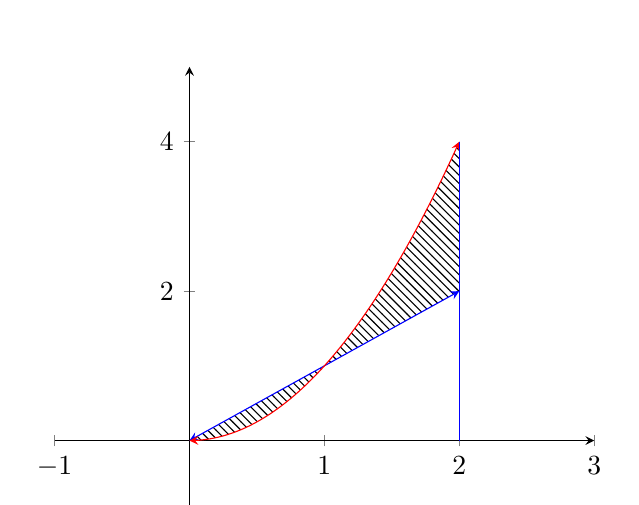
\begin{tikzpicture}[>=stealth]
   \begin{axis}[
        xmin=-1,xmax=3,
        ymin=-1,ymax=5,
        axis lines=middle,
        ]
        \addplot[no marks,blue,<->] expression[domain=0:2,samples=100, name path=A]{x};
	  \addplot[no marks,red,<->] expression[domain=0:2,samples=100, name path=B]{x^2};
	  \path[name path=xaxis] (\pgfkeysvalueof{/pgfplots/xmin}, 0) -- (\pgfkeysvalueof{/pgfplots/xmax}, 0);
	  \addplot[gray, pattern=north west lines] fill between[of=A and B, soft clip={domain=0:1}];
	  \addplot[gray, pattern=north west lines] fill between[of=B and A, soft clip={domain=1:2}];
	  \addplot +[mark=none] coordinates{(2, 0) (2, 4)};
    \end{axis}
\end{tikzpicture}
\end{center}
Let $V$ be the solid of revolution obtained by rotating $R$ about the $x$-axis. 

Note that $f_1, f_2$ are continuous on $[0, 2]$, hence $f_1, f_2 \in \mathcal{R}[0, 2]$. 

The volume of the part of $V$ between $x = 0$ and $x = 1$ is the difference of the volumes of the solids of revolution determined by $y = f_1$ and $y = f_2$. 

More precisely, since $f_1 \geq f_2$ on $[0, 1]$,
\begin{align*}
\text{Volume}(V \text{ restricted to } 0 \leq x \leq 1) & = \pi \int_0^1 f_1^2 - \pi \int_0^1 f_2^2 \\
& = \pi \int_0^1 x^2dx - \pi \int_0^1 (x^2)^2\,dx \\
& = \pi \int_0^1 (x^2 - x^4)\,dx \\
& = \pi \left[ \frac{x^3}3 - \frac{x^5}5\right]_{x=0}^{x=1} \\
& = \frac{2}{15}\pi
\end{align*}
Since $f_2 \geq f_1$ on $[1, 2]$,
\begin{align*}
\text{Volume}(V \text{ restricted to } 1 \leq x \leq 2) & = \pi \int_1^2 f_2^2 - \pi \int_1^2 f_1^2 \\
& = \pi \int_1^2 (x^4 - x^2)\,dx \\
& = \pi \left[\frac{x^5}5 - \frac{x^3}3\right]_{x=1}^{x=3} \\
& = \pi \left[\left(\frac{32}5 - \frac83\right) - \left(\frac15 - \frac13\right)\right] \\
& = \pi \left(\frac{31}5 - \frac73\right) = \frac{58}{15}\pi
\end{align*}
and so
$$\text{Volume}(V) = \frac{2}{15}\pi + \frac{58}{15}\pi = 4\pi \text{.}$$
Note that in general, we use
\begin{align*}
& \pi \int_a^b f_1^2 - f_2^2 \text{ where } f_1 \geq f_2 \geq 0 \\
& \pi \int_a^b f_2^2 - f_1^2 \text{ where } f_2 \geq f_1 \geq 0 
\end{align*}
so in general, 
$$\text{Volume}(V) = \pi \int_a^b \left|f_1^2 - f_2^2\right| \text{.}$$
\end{exmp}

% 4.4
\begin{exmp}
Find the volume of a ball of radius $r > 0$ in $\mbR^3$. 

Since the volume of the ball $B$ remains unchanged if we translate it, without loss of generality, we may assume that it is centred at the origin. In fact, if $\mbR$ is the region bounded by the curves
\begin{align*}
y & = \sqrt{r^2 - x^2} \\ y & = 0
\end{align*}
then the ball $B$ is the solid of revolution obtained by revolving $R$ about the $x$-axis. 

Hence
\begin{align*}
\text{Volume}(B) 
& = \pi \int_{-r}^r f^2 \\
& = \pi \int_{-r}^r (r^2 - x^2)\,dx \\
& = \pi \left[ r^2x - \frac{x^3}3\right]_{x=-r}^{x=r} \\
& = \pi \left[\left(r^3 - \frac{r^3}3\right) - \left(-r + \frac{r^3}3\right)\right] \\
& = \frac43\pi r^3
\end{align*}
Note that we can also consider the ball $B$ as the solid of revolution obtained by revolving the region $R'$ about the $y$-axis, where $R'$ is the region bounded by the curves 
\begin{align*}
x & = \sqrt{r^2 - y^2}, \hspace{5pt} y \in [-r, r] \\ x & = 0
\end{align*}
(in the $x$-$y$ plane) in which case we obtain
\begin{align*}
\text{Volume}(B) 
& = \pi \int_{-r}^r (\sqrt{r^2 - y^2})^2\,dy \\
& = \frac43\pi r^3 \text{.}
\end{align*}
Observe that in both cases, the variable with respect to which we are integrating coincides with the axis about which we revolve around the region.
\end{exmp}

% 4.5 
\begin{none}[The Shell Method]
In this method, we begin with a \underline{continuous} function $0 \leq f \in \zeta([a, b], \mbR)$, where $0 \leq a < b$. 

Let $R$ be the region bounded by the curves
\begin{align*}
y & = f(x) & x & = a \\ y & = 0 & x & = b
\end{align*}
Let $S$ be the solid of revolution obtained by revolving the region $R$ about the \underline{$y$-axis}. 

We approximate the volume of $S$ by the volume of a union of cylindrical shells obtained as follows: 

Let $P = \{a = p_0 < p_1 < \dots < p_N = b\} \in \mathcal{P}[a, b]$ and set
\begin{align*}
m_k & = \inf\{f(x) : x \in [p_{k-1}, p_k]\} \\
& = \min\{f(x) : x \in [p_{k-1}, p_k]\} = f(q_k^*) \text{ for some $q_k^* \in [p_{k-1}, p_k]$.} \\
M_k & = \sup\{f(x) : x \in [p_{k-1}, p_k]\} \\
& = \max\{f(x) : x \in [p_{k-1}, p_k]\} = f(q_k^{**}) \text{ for some $q_k^{**} \in [p_{k-1}, p_k]$.}
\end{align*}
for $1 \leq k \leq N$. 

Note that the union of the cylindical shells with base $[p_{k-1}, p_k]$ and height $m_k$ (respectively $M_k$) is contained in $S$ (respectively containing $S$). Thus,
\begin{align*} \sum_{k=1}^N \pi m_k(p_k^2 - p_{k-1}^2) & \leq \text{Volume}(S) \leq \sum_{k=1}^N \pi M_k(p_k^2 - p_{k-1}^2) & \text{(*)} \end{align*}
Neither the left hand side nor the right hand side look like a Riemann sum. 

Recall that if $g \in \mathcal{R}[a, b]$ and $P \in \mathcal{P}[a, b]$, then
$$\sum_{k=1}^N m_k(g, P)(p_k - p_{k-1}) \leq \int_a^b g \leq \sum_{k=1}^N M_k(g, P)(p_k - p_{k-1}) \text{.}$$
If $q_k \in [p_{k-1}, p_k]$ then $m_k \leq g(q_k) \leq M_k$, $1 \leq k \leq N$. Thus
$$L(g, P) \leq \sum_{k=1}^N g(q_k)(p_k - p_{k-1}) \leq U(g, P) \text{.}$$
Now consider the equation (*). We can rewrite it as
$$\pi \sum_{k=1}^N m_k(p_k + p_{k-1})(p_k - p_{k-1}) \leq \text{Volume}(S) \leq \pi \sum_{k=1}^N M_k(p_k + p_{k-1})(p_k - p_{k-1}) \text{.}$$
Consider
$$\pi \sum_{k=1}^N m_k (p_k + p_{k-1})(p_k - p_{k-1}) = \pi \left[ \sum_{k=1}^N m_k p_k (p_k - p_{k-1}) + \sum_{k=1}^N m_k p_{k-1} (p_k - p_{k-1})\right] \text{.}$$
Let $g(x) = x$, $x \in [a, b]$. Then $p_k = M_k(g, P) = g(p_k)$, $p_{k-1} = g(p_{k-1})$. 

Set $t_k^* = p_k$, $t_k^{**} = p_{k-1}$, so that $t_k^*, t_k^{**} \in [p_{k-1}, p_k]$. Then
\begin{align*}
\sum_{k=1}^N m_kp_k(p_k-p_{k-1}) & = \sum_{k=1}^N f(q_k^*)g(t_k^*)(p_k - p_{k-1}) \\
\sum_{k=1}^N m_kp_{k-1}(p_k-p_{k-1}) & = \sum_{k=1}^N f(q_k^*)g(t_k^{**})(p_k - p_{k-1})
\end{align*}
Now consider the following proposition: 

\textbf{Proposition.} Let $f, g \in \zeta([a, b], \mbR)$ and $\varepsilon > 0$. Then there exists $\delta > 0$ such that if $P \in \mathcal{P}[a, b]$ with $\norm{P} < \delta$, and if $y_k^*, z_k^* \in [p_{k-1}, p_k]$, $1 \leq k \leq N$, then
$$\left|\int_a^b fg - \sum_{k=1}^N f(y_k^*)g(z_k^*)(p_k - p_{k-1})\right| < \varepsilon \text{.}$$
\textbf{Proof.} On the assignment. $\qedsymbol$ 

From this, it follows that
$$\text{Volume}(S) = 2\pi\int_a^b fg = 2\pi\int_a^b xf(x) \hspace{2pt}dx \text{.}$$
\end{none}

% 4.6
\begin{exmp} Find the volume of $S$, where $S$ is the solid of revolution obtained by revolving the region $R$ about the $y$-axis, where $R$ is the region bounded by
\begin{align*} y & = f(x) = \sin x, \hspace{5pt} x \in [0, \pi] \\ y & = 0 \text{.} \end{align*}
From our work in 4.5,
$$\text{Volume}(S) = 2\pi\int_0^\pi x\sin x \hspace{2pt}dx \text{.}$$
We solve this using Integration by Parts. 
\[ \begin{aligned}
\text{Let } u & = x & dv & = \sin x \hspace{2pt}dx \\
du & = dx & v & = -\cos x
\end{aligned} \]
Then
\begin{align*}
\int x \sin x \hspace{2pt}dx
& = x(-\cos x) - \int -\cos x \hspace{2pt}dx \\
& = -x\cos x + \int \cos x \hspace{2pt}dx \\
& = -x\cos x + \sin x + \kappa, \hspace{5pt} \kappa \in \mbR 
\end{align*}
and thus
\begin{align*}
\text{Volume}(S)
& = 2\pi\int_0^\pi x \sin x \hspace{2pt}dx \\
& = 2\pi \biggr[-x\cos x + \sin x\biggr]_{x=0}^{x=\pi} \\
& = 2\pi^2 \text{.}
\end{align*}
\end{exmp}

% 4.7
\begin{remark}
Integration can also be used to calculate volumes of other objects, not necessarily obtained by revolving a region about an axis. 

For example, consider a pyramid with a square base with sides of length $b$ and height $h$. 

Again, the idea is to approximate the volume using ``slices''; in this case, we might want to use horizontal slices, since these are easiest to calculate. Using Leibniz's notation, and thinking of a slice as having thickness $\mathrm{d}x$, we need to figure out the volume of the slice at height $0 \leq x \leq h$. 

If $A_x$ is the area of the slice at height $h$, then by comparing triangles,
$$\frac{h-x}{b_x} = \frac{h}{b}$$
so $b_x = \dfrac{b}{h}(h-x)$ and $A_x = b_x^2 = \dfrac{b^2}{h^2}(h-x)^2$. 

The volume of each slice is $A_x\mathrm{d}x$, and so the volume of the pyramid is 
\begin{align*}
\int_0^h A_x \mathrm{dx}
& = \int_0^h \frac{b^2}{h^2}(h-x)^2 \, \mathrm{d}x \\
& = \frac{b^2}{h^2} \int_{t=h}^{t=0} t^2 (-\mathrm{d}t) \\
& = \frac{b^2}{h^2} \int_0^h t^2 \, \mathrm{d}t \\
& = \frac{b^2}{h^2} \left(\frac{h^3}3\right) \\
& = \frac13 b^2h \text{.}
\end{align*}
\end{remark}

\newpage

% Chapter 5
\section{Series}

% 5.1
\begin{none}
In this section, we are given an infinite sequence $(x_k)_{k=1}^\infty$ of real numbers which we would like to ``add''. Unfortunately, there is no way to do this. However, we can add finitely many at a time and take limits. Unlike finite sums, however, limits don't always behave nicely; first, the limit might not even exist, and secondly, even if it does, it might depend upon the order of the terms in the sequence.
\end{none}

% 5.2
\begin{defn}
Let $(x_k)_{k=1}^\infty$ be a sequence of real numbers. The symbol
$$\sum_{k=1}^\infty x_k$$
is \textbf{notation only}. It designates the sequence
$$\sum_{k=1}^\infty x_k \equiv (s_N)_{N=1}^\infty$$
of \textbf{partial sums} $s_N = \sum_{k=1}^N x_k$ of the $x_k$'s, in that specific order. We refer to $\sum_{k=1}^N x_k$ as a series in $(x_k)_{k=1}^\infty$. 

We say that the series $\sum_{k=1}^\infty x_k$ \textbf{converges} if $\lim_{N\to\infty} s_N$ exists. That is, if $(s_N)_{N=1}^\infty$ converges. We write $\sum_{k=1}^\infty x_k = \lim_{N\to\infty} s_N$. 

We also say that $\sum_{k=1}^\infty x_k$ \textbf{diverges} to $+\infty$ if $\lim_{N\to\infty} s_N = \infty$, and it diverges to $-\infty$ if $\lim_{N\to\infty} s_N = -\infty$.

If $\lim_{N\to\infty} s_N$ simply does not exist, we say that $\sum_{k=1}^\infty x_k$ diverges.
\end{defn}

% 5.3
\begin{exmp}~
\begin{enumerate}[(a)]

\item Let $0 \leq |p| \leq 1$. Observe that for $N > 1$,
$$1 + p + p^2 + \dots + p^N = \frac{1 - p^{N+1}}{1-p}$$
for $p \ne 1$.

Thus $$\sum_{k=0}^N p^k = 1 + \sum_{k=1}^N p_k = \dfrac{1 - p^{N+1}}{1-p} \text{,}$$
so $$\lim_{N\to\infty} \sum_{k=0}^N p^k = \lim_{N\to\infty} \frac{1-p^{N+1}}{1-p} = \frac{1}{1-p} \text{.}$$
We write $\sum_{k=0}^\infty p^k = \frac{1}{1-p}$.

In particular, we have
$$\sum_{k=0}^\infty \frac1{2^k} = \frac{1}{1/2} = 2 \text{.}$$
That is,
$$1 + \sum_{k=1}^\infty \frac1{2^k} = 2 \text{,}$$
or
$$\frac12 + \frac14 + \frac18 + \frac1{16} + \dots = 1 \text{.}$$
Similarly,
$$\frac13 + \frac19 + \frac1{27} + \dots = \frac12 \text{.}$$

\item $\sum_{k=1}^\infty (-1)^k$ diverges. 

Let $s_N = \sum_{k=1}^N (-1)^k = \begin{cases} -1 & \text{if $N$ is odd} \\ 0 & \text{if $N$ is even} \end{cases}$

Clearly $\lim_{N\to\infty} s_N$ does not exist.

\item If $p \geq 1$, then $\sum_{k=1}^\infty p^k$ diverges to $+\infty$.
\begin{itemize}
\item For $p = 1$, $s_N = N$, $N \geq 1$ so $\lim_{N\to\infty} s_N = \infty$.
\item For $p > 1$, $s_N = \frac{1-p^{N+1}}{1-p}$ and $\lim_{N\to\infty} s_N = \infty$.
\end{itemize}
\end{enumerate}
\end{exmp}

% 5.4
\begin{prop}[The Divergence Test]
Let $(x_k)_{k=1}^\infty$ be a sequence in $\mbR$. If $\sum_{k=1}^\infty x_k$ converges, then $\lim_{k\to\infty} x_k = 0$.
\end{prop}
\textbf{Proof.} 
Let $s_N = \sum_{k=1}^N x_k$, $N \geq 1$. If $\sum_{k=1}^\infty x_k$ converges, then $\lim_{N\to\infty} s_N = S$ exists. Hence $(s_N)_{N=1}^\infty$ is a Cauchy sequence, so given $\varepsilon > 0$ there exists $N_0 > 1$ such that $m, n \geq N_0$ implies $|s_m - s_n| < \varepsilon$. 

In particular, for $n \geq N_0$, 
$$|x_{n+1}| = |s_{n+1} - s_n| < \varepsilon$$
so that $\lim_{n\to\infty} x_n = 0$. $\qedsymbol$

% 5.5
\begin{caveat} 
The converse of Proposition 5.4 is false. If $(x_k)_{k=1}^\infty$ is a sequence in $\mbR$ and $\lim_{k\to\infty} x_k = 0$, it does not necessarily follow that $\sum_{k=1}^\infty x_k$ converges. 

For example, consider the harmonic series. 

Let $x_k = 1/k$, $k \geq 1$. Clearly, $\lim_{k\to\infty} x_k = 0$. Let $f(x) = 1/x$, $x > 0$. On the interval $[k, k+1]$, 
$$\frac1k \geq f(x) \text{,}$$
so by the Comparison Theorem for integrals,
\begin{align*}
s_N = \sum_{k=1}^N x_k & \geq \sum_{k=1}^N \int_k^{k+1} \frac1x \, \mathrm{d}x \\
& = \int_1^{N+1} \frac1x \, \mathrm{d}x = \ln(N+1) \text{.}
\end{align*}
Since $\lim_{N\to\infty} \ln(N+1) = \infty$, $\sum_{k=1}^\infty 1/k$ diverges to $\infty$. 

Note also that for $k \geq 1$, 
$$0 < \frac{1}{k+1} \leq f(x), \hspace{5pt} x \in [k, k+1] \text{,}$$
so by the Comparison Theorem,
$$\sum_{k=1}^N \frac{1}{k+1} \leq \sum_{k=1}^N \int_k^{k+1} \frac1x \, \mathrm{d}x = \ln(N+1) \text{.}$$
That is,
$$\frac12 + \frac13 + \dots + \frac1{N+1} \leq \ln(N+1) \text{,}$$
and
$$\ln(N+1) \leq 1 + \frac12 + \dots + \frac1N \leq \left(1 - \frac{1}{N+1}\right) + \ln(N+1) \text{.}$$
The harmonic series $\sum_{k=1}^\infty 1/k$ ``grows'' like $\ln(x)$.
\end{caveat}

% 5.6
\begin{prop}
Let $(x_k)_{k=1}^\infty \in \mbR^{\mbN}$ and suppose that $\gamma = \lim_{k\to\infty} x_k$ exists. Then
$$\sum_{k=1}^\infty (x_k - x_{k+1}) = x_1 - \gamma \text{.}$$
\end{prop}
\textbf{Proof.}
For each $N \geq 1$,
$$s_N := \sum_{k=1}^N (x_k - x_{k+1}) = x_1 - x_{N+1} \text{.}$$
But $\gamma = \lim_{k\to\infty} x_k = \lim_{N\to\infty} x_{N+1}$, and so
\begin{align*}
\sum_{k=1}^\infty (x_k - x_{k+1}) & = \lim_{N\to\infty} s_N \\
& = \lim_{N\to\infty} x_1 - x_{N+1} \\
& = x_1 - \gamma \text{. } \qedsymbol
\end{align*}

% 5.7
\begin{thm}[The Cauchy Criterion for Series]
Let $(x_k)_{k=1}^\infty \in \mbR^{\mbN}$. The following are equivalent:
\begin{enumerate}[(a)] \vspace{-0.2cm}
\item $\sum_{k=1}^\infty x_k$ converges.
\item For all $\varepsilon > 0$ there exists $N_0 \geq 1$ such that $m \geq n \geq N_0$ implies that
$$\left| \sum_{k=n+1}^m x_k \right| < \varepsilon \text{.}$$
\end{enumerate}
\end{thm}
\textbf{Proof.}
Note that $\sum_{k=1}^\infty x_k$ converges if and only if the sequence $(s_N)_{N=1}^\infty$ converges, where $s_N = \sum_{k=1}^N x_k$, $N \geq 1$, if and only if (by the Cauchy Criterion for sequences) for all $\varepsilon > 0$, there exists $N_0 \geq 1$ such that $m \geq n \geq N_0$ implies
$$\left| \sum_{k=n+1}^m x_k \right| = \left| \sum_{k=1}^m x_k - \sum_{k=1}^n x_k\right| = |s_m - s_n| < \varepsilon \text{. } \qedsymbol$$

% 5.8
\begin{cor}
Let $(x_k)_{k=1}^\infty \in \mbR^{\mbN}$. The following are equivalent:
\begin{enumerate}[(a)] \vspace{-0.2cm}
\item $\sum_{k=1}^\infty x_k$ converges.
\item For all $\varepsilon > 0$ there exists $N_1 \geq 1$ such that for all $n \geq N_1$, we have
$$\left| \sum_{k=n+1}^\infty x_k \right| < \varepsilon \text{.}$$
\end{enumerate}
\end{cor}
\textbf{Proof.}

(a) $\implies$ (b). Suppose that $\sum_{k=1}^\infty x_k$ converges, say $\sum_{k=1}^\infty x_k = \beta \in \mbR$. Let $s_N = \sum_{k=1}^N x_k$, $N \geq 1$, so that $\lim_{N\to\infty} s_N = \beta$.

Let $\varepsilon > 0$, and choose $N_1 \geq 1$ such that $n \geq N_1$ implies that
$$|s_n - \beta| < \varepsilon \text{.}$$
Note that 
\begin{align*}
\beta - s_n & = \sum_{k=1}^\infty x_k - \sum_{k=1}^n x_k \\
& = \lim_{N\to\infty} \sum_{k=1}^N x_k - \sum_{k=1}^n x_k \\
& = \lim_{N\to\infty} \sum_{k=n+1}^N x_k \\
& = \sum_{k=n+1}^\infty x_k \text{.}
\end{align*}
Hence $n \geq N_1$ implies that
$$|\beta - s_n| = \left|\sum_{k=n+1}^\infty x_k\right| < \varepsilon \text{.}$$
(b) $\implies$ (a). We will apply the Cauchy Criterion for series.

Let $\varepsilon > 0$. Choose $N_1 \geq 1$ such that for all $n \geq N_1$, we have
$$\left| \sum_{k=n+1}^\infty x_k\right| < \frac{\varepsilon}2 \text{.}$$
Suppose that $m \geq n \geq N_1$, so that
$$\left|\sum_{k=m+1}^\infty x_k \right| < \frac{\varepsilon}2 \text{ and } \left|\sum_{k=n+1}^\infty x_k\right| < \frac{\varepsilon}2 \text{.}$$
Consider
\begin{align*}
\left| \sum_{k=n+1}^m x_k\right| 
& = \left|\sum_{k=m+1}^\infty x_k - \sum_{k=n+1}^\infty x_k\right| \\
& \leq \left|\sum_{k=m+1}^\infty x_k\right| + \left|\sum_{k=n+1}^\infty x_k\right| \\
& < \frac{\varepsilon}2 + \frac{\varepsilon}2 = \varepsilon \text{.}
\end{align*}
By the Cauchy Criterion for series, $\sum_{k=1}^\infty x_k$ converges. $\qedsymbol$

% 5.9
\begin{prop}
Let $(x_k)_{k=1}^\infty$, $(y_k)_{k=1}^\infty \in \mbR^{\mbN}$ and $\alpha \in \mbR$. 

If $\sum_{k=1}^\infty x_k$ converges to $\beta_x \in \mbR$ and $\sum_{k=1}^\infty y_k$ converges to $\beta_y \in \mbR$, then
\begin{enumerate}[(a)] \vspace{-0.2cm}
\item $\sum_{k=1}^\infty (x_k + y_k)$ converges to $\beta_x + \beta_y$. 
\item $\sum_{k=1}^\infty (\alpha x_k) = \alpha \left(\sum_{k=1}^\infty x_k\right) = \alpha \beta_x$.
\end{enumerate}
\end{prop}
\textbf{Proof.} 
\begin{enumerate}[(a)] \vspace{-0.2cm}
\item Let $s_N = \sum_{k=1}^N x_k$, $t_N = \sum_{k=1}^N y_k$, $N \geq 1$, so that $\lim_{N\to\infty} s_N = \beta_x$ and $\lim_{N\to\infty} t_N = \beta_y$. 
Recall that
\begin{align*}
\beta_x + \beta_y & = \lim_{N\to\infty} s_N + \lim_{N\to\infty} t_N \\
& = \lim_{N\to\infty} (s_N + t_N)
\end{align*}
since both limits exist.

But for all $N \geq 1$,
\begin{align*}
s_N + t_N & = \sum_{k=1}^N x_k + \sum_{k=1}^N y_k \\ & = \sum_{k=1}^N (x_k + y_k)
\end{align*}
Hence $\beta_x + \beta_y = \lim_{N\to\infty} \sum_{k=1}^N (x_k + y_k) = \sum_{k=1}^\infty (x_k + y_k)$.
\item Left as an exercise. $\qedsymbol$
\end{enumerate}

% 5.10
\begin{caveat}
The converse of Proposition 5.9 is false. 

For example, let $x_k = 1$, $y_k = -1$ for $k \geq 1$. 
Then $\sum_{k=1}^\infty (x_k + y_k) = \sum_{k=1}^\infty (0) = 0$, but $\sum_{k=1}^\infty x_k$ and $\sum_{k=1}^\infty y_k$ diverge to $+\infty$ and $-\infty$, respectively.
\end{caveat}

% 5.11
\begin{none}
It is worth noting that the convergence of a series $\sum_{k=1}^\infty x_k$ has nothing to do with \underline{finitely} many terms in the series. 

Suppose that $(x_k)_{k=1}^\infty \in \mbR^{\mbN}$ is a sequence and that $(P)$ is a property that each $x_k$ may or may ot have. 

We say that $(P)$ holds for large $k$ (for $(x_k)_{k=1}^\infty$) to mean that there exists $N \geq 1$ such that $k \geq N$ implies that $x_k$ has property $(P)$. 

We can also extend this to properties of the terms in pairs of sequences. 

If $(P)$ is a property between pairs of real numbers (that may or may not hold), we say that $(P)$ holds for large $k$ \underline{relative} to $(x_k)_{k=1}^\infty$ and $(y_k)_{k=1}^\infty$ if there exists $N \geq 1$ such that $k \geq N$ implies that the pair $(x_k, y_k)$ has property $(P)$. 

As another example, say $(P)$ is the property that $x \leq y$. Given $(x_k)_{k=1}^\infty$, $(y_k)_{k=1}^\infty \in \mbR^{\mbN}$, we say that $(P)$ holds for large $k$ if there exists $N \geq 1$ such that $x_k \leq y_k$ for all $k \geq N$. 

Suppose that $x_k = y_k$ for large $k$. We claim that $\sum_{k=1}^\infty x_k$ converges if and only if $\sum_{k=1}^\infty y_k$ converges. 

Let $s_N = \sum_{k=1}^N x_k$ and $t_N = \sum_{k=1}^N y_k$. 

Let $\beta_x = \lim_{N\to\infty} s_N$ and $\beta_y = \lim_{N\to\infty} t_N$. 

Choose $N_0 \geq 1$ such that $k \geq N_0$ implies that $x_k = y_k$. 
Then, with $N \geq N_0$, 
\begin{align*}
|s_N - t_N| 
& = \left|\sum_{k=1}^N x_k - \sum_{k=1}^N y_k\right| \\
& = \Bigg| \left(\sum_{k=1}^{N_0 - 1} x_k - \sum_{k=1}^{N_0 - 1} y_k \right) + \underbrace{\left(\sum_{k=N_0}^N x_k - \sum_{k=N_0}^N y_k\right)}_{0}\Bigg| \\
& =  \underbrace{\left|\sum_{k=1}^{N_0 - 1} (x_k - y_k)\right|}_{\text{constant}}
\end{align*}
But since $|s_N - t_N|$ is constant for all $N \geq N_0$, $(s_N)_{N=1}^\infty$ converges if and only if $(t_N)_{N=1}^\infty$ converges.
\end{none}

% 5.12
\begin{thm}
Let $(x_k)_{k=1}^\infty$ with $x_k \geq 0$ for all $k \geq 1$. The following are equivalent:
\begin{enumerate}[(a)] \vspace{-0.2cm}
\item $\sum_{k=1}^\infty x_k$ converges.
\item $(s_N)_{N_1}^\infty$ is bounded above.
\end{enumerate}
\end{thm}
\textbf{Proof.}

(a) $\implies$ (b). Let $s_N = \sum_{k=1}^N x_k$. Since $\sum_{k=1}^\infty x_k$ converges, $\lim_{N\to\infty} s_N$ exists. Hence $(s_N)_{N=1}^\infty$ is bounded. 

(b) $\implies$ (a). Suppose that $(s_N)_{N_1}^\infty$ is bounded (hence bounded above). Note that for all $N \geq 1$,
\begin{align*}
s_{N+1} - s_N & = \sum_{k=1}^{N+1} x_k - \sum_{k=1}^N x_k \\ & = x_{N+1} \\ & \geq 0 \text{.}
\end{align*}
Thus $(s_N)_{N=1}^\infty$ is increasing. 

Hence $\sum_{k=1}^\infty x_k = \lim_{N\to\infty} s_N = \sup_{N\geq 1} s_N < \infty$, so $\sum_{k=1}^\infty x_k$ converges. $\qedsymbol$

% INDENT
%\setlength\parindent{15pt}

% 5.13 
\begin{none}[The Integral Test]
Suppose that $f: [1, \infty) \to [0, \infty)$ is a monotone decreasing function. The following are equivalent:
\begin{enumerate}[(a)] \vspace{-0.2cm}
\item $\sum_{k=1}^\infty f(k)$ converges (i.e. $\sum_{k=1}^\infty f(k) < \infty$)
\item $\int_1^\infty f$ converges (i.e. $\int_1^\infty f < \infty$)
\end{enumerate}
\end{none}
\textbf{\small Proof.} Observe that since $f$ is monotone decreasing on $[1, \infty)$, then if $[a, b] \subseteq [1, \infty)$ is any closed, bounded interval in $[1, \infty)$, then $f$ is monotone decreasing on $[a, b]$, hence integrable on $[a, b]$. That is, $f$ is locally integrable on $[1, \infty)$. 

Let 
\begin{align*} 
g(x) & = \begin{cases} f(k+1) & x \in (k, k+1] \\ f(2) & x = 1 \end{cases} \\
h(x) & = f(k) \hspace{10pt} x \in [k, k+1) 
\end{align*}
for $1 \leq k$. 

Note that each of $g, h$ are piecewise constant on $[1, \infty)$, and so they are locally integrable on $[1, \infty)$. 

Moreover, $g(x) \leq f(x) \leq h(x)$ for all $x \in [1, \infty)$, so by the Comparison Theorem for Integrals, for each $N \geq 1$,
$$f(2) + \dots + f(N) = \int_1^N g \leq \int_1^N f \leq \int_1^N h = f(1) + \dots + f(N-1).$$
That is,
$$\sum_{k=2}^N f(k) \leq \int_1^N f \leq \sum_{k=1}^{N-1} f(k)$$
for all integers $N \geq 2$. 

(a) $\implies$ (b). Suppose $\sum_{k=1}^\infty f(k) < \infty$. Then, since $0 \leq f(j)$ for all $j \geq 1$,
$$\int_2^N f \leq \sum_{k=1}^{N-1} f(k) \leq \sum_{k=1}^\infty f(k) =: \beta < \infty$$
Observe that if 
$$F(x) = \int_1^x f(t) \, dt$$
then $F$ is increasing on $[1, \infty)$ (since $f \geq 0$ on $[1, \infty)$). As such,
\begin{align*}
\int_1^\infty f(t)\,dt & = \lim_{x\to\infty} \int_1^x f(t)\,dt \\
& = \sup_{x \geq 1} \int_1^x f(t)\,dt \\
& = \sup_{N\geq2, N\in\mbN} \int_1^N f(t)\,dt \\
& \leq \beta = \sum_{k=1}^\infty f(k) < \infty
\end{align*}
Thus $\int_1^\infty f(t)\,dt < \infty$. 

(b) $\implies$ (a). Suppose $\int_1^\infty f(t)\,dt < \infty$. From above, for all $N \geq 2$, $N \in \mbN$,
\begin{align*}
s_N := \sum_{k=1}^N f(k) & = f(1) + \sum_{k=2}^N f(k) \\
& \leq f(1) + \int_1^N f(t)\,dt \\
& \leq \underbrace{f(1) + \int_1^\infty f(t)\,dt}_{\text{constant}} < \infty
\end{align*}
Thus $(s_N)_{N=1}^\infty$ is an increasing sequence and $(s_N)_{N=1}^\infty$ is bounded above, and so
$$\sum_{k=1}^\infty f(k) = \lim_{N\to\infty} s_N = \sup_{N\geq1} s_N \leq f(1) + \int_1^\infty f(t)\,dt < \infty. \text{ } \qedsymbol$$

% 5.14
\begin{cor}[The $p$-Test for Series]
The series $\sum_{k=1}^\infty 1/k^p$ converges if and only if $p > 1$.
\end{cor}
\textbf{\small Proof.} Exercise. $\qedsymbol$

% 5.15
\begin{none}[The Comparison Test]
Suppose that $0 \leq a_k \leq b_k$ for large $k$. If $\sum_{k=1}^\infty b_k < \infty$, then $\sum_{k=1}^\infty a_k < \infty$. 

Hence if $\sum_{k=1}^\infty a_k$ diverges, so does $\sum_{k=1}^\infty b_k$.
\end{none}
\textbf{\small Proof.} We are only interested in whether the series converges or diverges, so without loss of generality, assume that $0 \leq a_k \leq b_k$ holds for all $k \geq 1$. 

For each $N \geq 1$, 
$$s_N := \sum_{k=1}^N a_k \leq \sum_{k=1}^N b_k \leq \sum_{k=1}^\infty b_k =: \beta < \infty$$
But $a_k \geq 0$ for all $k \geq 1$, so $(s_N)_{N=1}^\infty$ is an increasing sequence bounded above by $\beta = \sum_{k=1}^\infty b_k$. 

Hence
$$\sum_{k=1}^\infty a_k := \lim_{N\to\infty} s_N = \sup_{N\geq1} s_N \leq \beta < \infty. \text{ } \qedsymbol$$

% 5.16
\begin{exmp}~
\begin{enumerate}[(a)] \vspace{-0.2cm}

\item Consider $\sum_{k=1}^\infty \frac{k^3 \log^2 k}{e^k}$. We show that this converges.

Note that if $a_k := \frac{k^3\log^2k}{e^k}$, then
$$0 \leq a_k \leq b_k := \frac{k^3 \cdot k^2}{e^k} = \frac{k^5}{e^k}.$$
By the Comparison Test for Series, it suffices to show that $\sum_{k=1}^\infty b_k < \infty$. 

Let us write $h(x) = \frac{x^5}{e^{x/2}}$. Then $b_k = h(x) \cdot \frac{1}{(\sqrt{e})^k}$, $k \geq 1$. Then
\begin{align*}
\lim_{x\to\infty} h(x) & = \lim_{x\to\infty} \frac{x^5}{e^{x/2}} \\
& \lhr \lim_{x\to\infty} \frac{5x^4}{(1/2)e^{x/2}} \\
& \lhr \lim_{x\to\infty} \frac{20x^3}{(1/2)^2 e^{x/2}} \\
& \lhr \lim_{x\to\infty} \frac{60x^2}{(1/2)^3 e^{x/2}} \\
& \lhr \lim_{x\to\infty} \frac{120x}{(1/2)^4 e^{x/2}} \\
& \lhr \lim_{x\to\infty} \frac{120}{(1/2)^5 e^{x/2}} = 0
\end{align*}
hence $\lim_{x\to\infty} h(x)$ exists, and it follows that
$\lim_{x\to\infty} \frac{x^5}{e^{x/2}} = 0$.

Now fix $N_0 \geq 1$ so that $x \geq N_0$ implies that $\frac{x^5}{e^{x/2}} < 1$. If $k \geq N_0$, $k \in \mbZ$, then
\begin{align*}
b_k = \frac{k^5}{e^k} & = \frac{k^5}{e^{k/2}} \frac{1}{e^{k/2}} \\
& < 1 \cdot \frac{1}{e^{k/2}} = \left(\frac{1}{\sqrt{e}}\right)^k
\end{align*}
Hence for large $k$,
$$b_k \leq \frac{1}{(\sqrt{e})^k}$$
and $\sum_{k=1}^\infty \frac{1}{(\sqrt{e})^k} < \infty$ since it is a geometric series with $1/\sqrt{e} < 1$. 

By the Comparison Test for series, 
$$\sum_{k=1}^\infty b_k < \infty$$
and applying the Comparison Test again,
$$\sum_{k=1}^\infty a_k < \infty$$
That is,
$$\sum_{k=1}^\infty \frac{k^3\log^2k}{e^k} < \infty.$$

\item Consider $\sum_{k=1}^\infty \frac{1}{k^{\log k}}$. Note that for $k \geq 9$, $\log k \geq 2$, so
$$\frac{1}{k^{\log k}} \leq \frac{1}{k^2}$$
By the $p$-test, $\sum_{k=1}^\infty \frac{1}{k^2}$ converges. Then by the Comparison Test for series, $\sum_{k=1}^\infty \frac{1}{k^{\log k}}$ converges as well.

\end{enumerate}
\end{exmp}

% 5.17
\begin{none}[The Limit Comparison Test]
Suppose that $0 \leq a_k \leq b_k$ for large $k$ and that $L := \lim_{k\to\infty} a_k/b_k$ exists in $[0, \infty) \cup \{\infty\}$.
\begin{enumerate}[(a)] \vspace{-0.2cm}
\item If $0 < L < \infty$, then $\sum_{k=1}^\infty a_k$ converges if and only if $\sum_{k=1}^\infty b_k$ converges.
\item If $L = 0$ and $\sum_{k=1}^\infty b_k$ converges, then $\sum_{k=1}^\infty a_k$ converges.
\item If $L = \infty$ and $\sum_{k=1}^\infty b_k = \infty$, then $\sum_{k=1}^\infty a_k = \infty$.
\end{enumerate}
\end{none}
\textbf{Proof.} 
\begin{enumerate}[(a)] \vspace{-0.2cm}

\item With $0 < L < \infty$, choose $N_1 \geq 1$ such that $k \geq N_1$ implies that $\frac12 \leq \frac{a_k}{b_k} \leq 2L$. That is, $\frac12b_k \leq a_k \leq (2L)b_k$. 

Now if $\sum_{k=1}^\infty b_k < \infty$, then $\sum_{k=1}^\infty (2L)b_k < \infty$. By the Comparison Test, $\sum_{k=1}^\infty a_k < \infty$. 

If $\sum_{k=1}^\infty b_k = \infty$, then $\sum_{k=1}^\infty \frac12b_k = \infty$. By the Comparison Test, $0 \leq \frac12b_k \leq a_k$ for large $k$ implies that $\sum_{k=1}^\infty a_k = \infty$. 

\item If $L = 0$, then we can choose $N_2 \geq 1$ such that $k \geq N_2$ implies that $a_k, b_k \geq 0$ and $a_k / b_k < 1$. That is, $a_k < b_k$. By the Comparison Test, $\sum_{k=1}^\infty b_k < \infty$ implies that $\sum_{k=1}^\infty a_k < \infty$.

\item Similar to (b). $\qedsymbol$

\end{enumerate}

% 5.18
\begin{exmp}
Suppose $(a_k)_{k=1}^\infty \in \mbR^\mbN$ and $\lim_{k\to\infty} |a_k| = 0$. Observe that
$$\lim_{k\to\infty} \frac{\sin|a_k|}{|a_k|} = 1,$$
so by the Limit Comparison Test, $\sum_{k=1}^\infty |a_k| < \infty$ if and only if $\sum_{k=1}^\infty \sin|a_k| < \infty$.
\end{exmp}

% 5.19
We now turn our attention to series where infinitely many terms may be negative. The strongest notion of convergence is the following:

\begin{defn}
Let $\sum_{k=1}^\infty x_k$ be an infinite series. We say that the series \textbf{converges absolutely} if $\sum_{k=1}^\infty |x_k|$ converges. 

If $\sum_{k=1}^\infty x_k$ converges but is \textbf{not} absolutely convergent, then we say that $\sum_{k=1}^\infty x_k$ converges conditionally.
\end{defn}

% 5.20
\begin{exmp}
Examples of absolute and conditional convergence:
\begin{enumerate}[(a)]
\item If $x_k \geq 0$ for large $k$ and $\sum_{k=1}^\infty x_k$ converges, then $\sum_{k=1}^\infty x_k$ converges absolutely. 
\item We have seen that $\sum_{k=1}^\infty 1/k^2$ converges, so if $x_k = (-1)^k/k^2$, then $\sum_{k=1}^\infty x_k$ converges absolutely. 
\item We have seen that $\sum_{k=1}^\infty 1/k$ diverges, while the alternating harmonic series $\sum_{k=1}^\infty (-1)^k/k$ converges. Thus, the alternating harmonic series converges conditionally.
\end{enumerate}
\end{exmp}

% 5.21
From the Cauchy Criterion for series, we get the following:
\begin{prop}
Let $\sum_{k=1}^\infty x_k$ be a series. The following are equivalent:
\begin{enumerate}[(a)] \vspace{-0.2cm}
\item $\sum_{k=1}^\infty x_k$ converges absolutely.
\item For all $\varepsilon > 0$ there exists $N > 0$ such that $m > n \geq N$ implies $\sum_{k=n+1}^m |x_k| < \varepsilon$. 
\end{enumerate}
\end{prop}

% 5.22
\begin{prop}
If the series $\sum_{k=1}^\infty x_k$ converges absolutely, then $\sum_{k=1}^\infty x_k$ converges.
\end{prop}
\textbf{Proof.} We shall apply the Cauchy Criterion for series. Suppose $\sum_{k=1}^\infty x_k$ converges absolutely and let $\varepsilon > 0$. Choose $N > 0$ such that $m > n \geq N$ implies $\sum_{k=n+1}^m |x_k| < \varepsilon$. 

Then $m > n \geq N$ implies
$$\left| \sum_{k=n+1}^m x_k \right| \leq \sum_{k=n+1}^m |x_k| < \varepsilon$$
so that by the Cauchy Criterion, $\sum_{k=1}^\infty x_k$ converges. $\qedsymbol$ 

% 5.23
Recall the following definition from {\sc Math 147}: 
\begin{defn}
Given a sequence $(x_k)_{k=1}^\infty \in \mbR^\mbN$, the \textbf{limit supremum} of $(x_k)_{k=1}^\infty$ is
$$\limsup_{n\to\infty} x_n := \lim_{n\to\infty} \left(\sup_{k\geq n} x_k\right) \in \mbR \cup \{\pm\infty\}$$
while the \textbf{limit infimum} of $(x_k)_{k=1}^\infty$ is
$$\liminf_{n\to\infty} x_n := \lim_{n\to\infty} \left(\inf_{k\geq n} x_n \right) \in \mbR \cup \{\pm\infty\}$$
Recall also that with $\beta \in \mbR$, 
\begin{enumerate}[(a)] \vspace{-0.2cm}
\item if $\limsup_{k\to\infty} x_k < \beta < \infty$, then $x_k < \beta$ for large $k$.
\item if $\limsup_{k\to\infty} x_k > \beta$, then there exist $n_1 < n_2 < \dots$ so that $x_{n_j} > \beta$, $j \geq 1$.
\item if $\lim_{k\to\infty} x_k = \beta$, then $\limsup_{k\to\infty} x_k = \liminf_{k\to\infty} x_k = \beta$.
\end{enumerate}
\end{defn}

% 5.24
\begin{thm}[The Root Test]
Let $(x_k)_{k=1}^\infty \in \mbR^\mbN$ and let $\rho := \limsup_{k\to\infty} |x_k|^{1/k}$. 
\begin{enumerate}[(a)] \vspace{-0.2cm}
\item if $\rho < 1$, then $\sum_{k=1}^\infty x_k$ converges absolutely.
\item if $\rho > 1$, then $\sum_{k=1}^\infty x_k$ diverges.
\end{enumerate}
\end{thm}
\textbf{Proof.} 

\begin{enumerate}[(a)] \vspace{-0.2cm}

\item Let $\beta = \frac{1+\rho}2$, so that $\rho < \beta < 1$. 

Then $\limsup_{k\to\infty} |x_k|^{1/k} < \beta$, so from above, we see that $|x_k|^{1/k} < \beta$; that is, $|x_k| < \beta^k$ for large $k$. Since $\beta < 1$, $\sum_{k=1}^\infty \beta^k$ converges. By the Comparison Test for series, $\sum_{k=1}^\infty |x_k|$ converges, or $\sum_{k=1}^\infty x_k$ converges absolutely.

\item Let $\gamma = \frac{1+\rho}2$ so that $1 < \gamma < \rho$. 

Then $\limsup_{k\to\infty} |x_k|^{1/k} > \gamma$, so from above, we can find $n_1 < n_2 < \dots$ so that $|x_k|^{1/k} > \gamma > 1$. Thus $|x_k| > 1$, and by the Divergence Test, $\sum_{k=1}^\infty x_k$ diverges. $\qedsymbol$

\end{enumerate}

% 5.25
\begin{none}
The Root Test gives no information when $\rho = 1$. Note that $\sum_{k=1}^\infty 1/k$ diverges, while $\sum_{k=1}^\infty 1/k^2$ converges by the $p$-Test.

Let $x_k = 1/k$, $y_k = 1/k^2$. Then $|x_k|^{1/k} = \left(\frac1k\right)^{1/k} = \frac{1}{k^{1/k}} = k^{-1/k}$.

To find $\lim_{k\to\infty} k^{-1/k}$, we can consider $\log(x^{-1/x}) = -\frac1x\log x$. Then
$$\lim_{x\to\infty} \log(x^{-1/x}) = \lim_{x\to\infty} -\frac{\log x}x \lhr \lim_{x\to\infty} \frac{-1/x}1 = 0$$
so $\lim_{k\to\infty} k^{-1/k} = e^0 = 1$. 
	
Hence $\lim_{k\to\infty} |x_k|^{1/k} = 1$, and $\sum_{k=1}^\infty x_k$ diverges. 

On the other hand, $y_k = x_k^2$, so
\begin{align*}
\lim_{k\to\infty} |y_k|^{1/k} & = \lim_{k\to\infty} \left(|x_k|^{1/k}\right)^2 \\
& = \left(\lim_{k\to\infty} |x_k|^{1/k}\right)^2 \\
& = 1^2 = 1
\end{align*}
while $\sum_{k=1}^\infty y_k$ converges.
\end{none}

% 5.26
\begin{thm}[The Ratio Test]
Let $(x_k)_{k=1}^\infty \in \mbR^\mbN$ and assume that $x_k \ne 0$ for large $k$. If 
$$\rho := \lim_{k\to\infty} \left| \frac{x_{k+1}}{x_k} \right|$$
exists in $\mbR \cup \{\infty\}$, then we have the following:
\begin{enumerate}[(i)] \vspace{-0.2cm}
\item If $\rho < 1$, then $\sum_{k=1}^\infty x_k$ converges absolutely.
\item If $\rho > 1$, then $\sum_{k=1}^\infty x_k$ diverges.
\end{enumerate}
\end{thm}

\textbf{Proof.} 
\begin{enumerate}[(i)] \vspace{-0.2cm}

\item Suppose that $\rho < 1$. If $\beta \in (\rho, 1)$, each term will eventually have $\left| \frac{x_{k+1}}{x_k} \right| < \beta$. 
Pick $N$ so that $n \geq N$ implies $\left| \frac{x_{n+1}}{x_n} \right| < \beta$. In particular,
$$\left| \frac{x_{N+1}}{x_N} \right| < \beta \implies |x_{n+1}| < \beta|x_n|$$
Also,
$$\left| \frac{x_{N+2}}{x_{N+1}} \right| < \beta \implies |x_{N+2}| < \beta|x_{N+1}| < \beta^2|x_N|$$
By induction, we have that
$$|x_{N+i}| < \beta^i |x_N|$$
Hence
$$\sum_{k=N+1}^\infty |x_k| = \sum_{k=1}^\infty |x_{N+k}| < \sum_{k=1}^\infty \beta^k |x_N| = |x_N| \sum_{k=1}^\infty \beta_k < \infty$$
since $\sum_{k=1}^\infty \beta^k$ is a geometric series and $\beta < 1$. Therefore, $\sum_{k=1}^\infty x_k$ converges absolutely. 

\item Suppose $\rho > 1$. Choose $\beta \in (1, \rho)$ and note that for all $n \geq N$, it must be that $\left| \frac{x_{n+1}}{x_n} \right| > \beta$. From this, we can show that for all $i$,
$$|x_{N+i}| > \beta^i|x_N|$$
Hence
$$|x_{N+i}| > \underbrace{\beta^i}_{>1} |x_N| > |x_N| > 0$$
Thus the terms do not go to 0. Hence by the Divergence Test, $\sum_{k=1}^\infty x_k$ diverges. $\qedsymbol$

\end{enumerate}

\textbf{Exercise.} Use the Ratio Test to determine if $\sum_{k=1}^\infty \frac{k^5}{e^k}$ converges.

% 5.27
\begin{none}
If $\rho = 1$ in the Ratio Test, we obtain no information. 
For example, $\sum_{k=1}^\infty 1/k$ diverges, yet
$$\rho = \lim_{k\to\infty} \frac{1/(k+1)}{1/k} = \lim_{k\to\infty} \frac{k}{k+1} = 1$$
On the other hand, $\sum_{k=1}^\infty 1/k^2$ converges, and
$$\rho = \lim_{k\to\infty} \frac{1/(k+1)^2}{1/k^2} = \lim_{k\to\infty} \frac{k^2}{(k+1)^2} = 1$$
\end{none}

% 5.28
\begin{defn}
Let $(x_k)_{k=1}^\infty \in \mbR^\mbN$. A series $(y_k)_{k=1}^\infty$ is said to be a \textbf{rearrangement} of $\sum_{k=1}^\infty x_k$ if there is a bijective map $\sigma : \mbN \to \mbN$ such that $y_k = x_{\sigma(k)}$ for all $k$.
\end{defn}

Note that on A1Q6, we proved that if $\sum_{k=1}^\infty x_k$ is a convergent series of positive terms, then any rearrangement $\sum_{k=1}^\infty y_k$ of this series is also convergent, and
$$\sum_{k=1}^\infty x_k = \sum_{k=1}^\infty y_k$$

% 5.29
\begin{prop}
If $\sum_{k=1}^\infty x_k$ is an absolutely convergent series and $\sum_{k=1}^\infty y_k$ is some rearrangement of $\sum_{k=1}^\infty x_k$, then $\sum_{k=1}^\infty y_k$ is absolutely convergent, and
$$\sum_{k=1}^\infty x_k = \sum_{k=1}^\infty y_k$$
\end{prop}
\textbf{Proof.} Let $\sigma : \mbN \to \mbN$ be a bijective function, so that
$$y_k = x_{\sigma(k)}$$
Since $\sum_{k=1}^\infty x_k$ converges absolutely, by definition, we have that $\sum_{k=1}^\infty |x_k|$ converges. 

By A1Q6, we have that $\sum_{k=1}^\infty |x_{\sigma(k)}|$ converges (sum of positive terms).

Therefore $\sum_{k=1}^\infty |y_k|$ converges, so $\sum_{k=1}^\infty y_k$ converges absolutely. 

Suppose that $\beta = \sum_{k=1}^\infty y_k$. Let $\varepsilon > 0$, and choose $M \in \mbN$ such that
\begin{enumerate}[(a)]
\item $\left| \beta - \displaystyle\sum_{k=1}^M y_k \right| < \dfrac{\varepsilon}2$
\item $\displaystyle\sum_{k=M+1}^\infty |y_k| < \dfrac{\varepsilon}2$
\end{enumerate}
Finally, choose $N = \max\{\sigma(1), \sigma(2), \dots, \sigma(M)\}$ so that
\begin{align*}
\{y_1, \dots, y_M\} & = \{x_{\sigma(1)}, \dots, x_{\sigma(M)}\} \\ & \subseteq \{x_1, \dots, x_N\}
\end{align*}
We claim that when $n \geq N$, we have
$$\left| \beta - \sum_{k=1}^n x_k \right| < \varepsilon$$
Indeed, for $n \geq N$, if we define $A_n = \{1, \dots, n\} \setminus \{\sigma(1), \dots, \sigma(M)\}$,
\begin{align*}
\left| \beta - \sum_{k=1}^n x_k \right| & = \left| \beta - \sum_{k=1}^M x_{\sigma(k)} - \sum_{k \in A_n} x_k \right| \\
& \leq \left| \beta - \sum_{k=1}^M y_k \right| + \sum_{k \in A_n} |x_k|
\end{align*}
Note that if $k \in A_n$, then $x_k = y_j = x_{\sigma(j)}$ for some $j \geq M+1$. So
\begin{align*}
\left| \beta - \sum_{k=1}^n x_k \right| & < \frac{\varepsilon}2 + \sum_{j=M+1}^\infty |x_{\sigma(j)}| \\
& < \frac{\varepsilon}2 + \frac{\varepsilon}2 = \varepsilon
\end{align*}
Therefore,
$$\sum_{k=1}^\infty x_k = \beta = \sum_{k=1}^\infty y_k \text{ } \qedsymbol$$

% 5.30
\begin{notation}
Given $x \in \mbR$, define
\begin{align*}
x^+ & = \max(x, 0) \\
x^- & = \max(-x, 0)
\end{align*}
\end{notation}

We can find the following properties:
\begin{enumerate}
\item $x^+, x^- \geq 0$
\item $x^+ + x^- = |x|$
\item $x^+ - x^- = x$
\end{enumerate}
From 2 and 3, we can deduce
\begin{enumerate}[resume]
\item $x^+ = \dfrac{x+|x|}2$
\item $x^- = \dfrac{-x+|x|}2$
\end{enumerate}

% 5.31
\begin{prop}
Let $(x_k)_{k=1}^\infty \in \mbR^\mbN$.

\begin{enumerate}[(a)] \vspace{-0.2cm}

\item If $\sum_{k=1}^\infty x_k$ converges absolutely, then so do $\sum_{k=1}^\infty x_k^+$ and $\sum_{k=1}^\infty x_k^-$. Moreover, we have
\begin{align*}
\sum_{k=1}^\infty |x_k| & = \sum_{k=1}^\infty x_k^+ + \sum_{k=1}^\infty x_k^- \\
\sum_{k=1}^\infty x_k & = \sum_{k=1}^\infty x_k^+ - \sum_{k=1}^\infty x_k^-
\end{align*}

\item If $\sum_{k=1}^\infty x_k$ converges conditionally, then $\sum_{k=1}^\infty x_k^+$ and $\sum_{k=1}^\infty x_k^-$ diverge to $\infty$.

\end{enumerate}
\end{prop}
\textbf{Proof.} 

\begin{enumerate}[(a)] \vspace{-0.2cm}

\item Suppose $\sum_{k=1}^\infty x_k$ converges absolutely. Since $x_k^+, x_k^- \leq |x_k|$, we have from the Comparison Test that $\sum_{k=1}^\infty x_k^+$ and $\sum_{k=1}^\infty x_k^-$ converge (absolutely). 

Moreover, since $|x_k| = x_k^+ + x_k^-$, we have
\begin{align*}
\sum_{k=1}^\infty |x_k| & = \sum_{k=1}^\infty (x_k^+ + x_k^-) \\
& = \sum_{k=1}^\infty x_k^+ + \sum_{k=1}^\infty x_k^-
\end{align*}
Likewise,
\begin{align*}
\sum_{k=1}^\infty x_k & = \sum_{k=1}^\infty (x_k^+ - x_k^-) \\
& = \sum_{k=1}^\infty x_k^+ - \sum_{k=1}^\infty x_k^-
\end{align*}

\item Suppose that $\sum_{k=1}^\infty x_k$ converges conditionally, and to the contrary, also suppose that $\sum_{k=1}^\infty x_k^+$ converges. We have
\begin{align*}
\sum_{k=1}^\infty x_k^- & = \sum_{k=1}^\infty (x_k^+ - x_k) \\
& = \sum_{k=1}^\infty x_k^+ - \sum_{k=1}^\infty x_k
\end{align*}
Since these series both converge, $\sum_{k=1}^\infty x_k^-$ also converges. This means
\begin{align*}
\sum_{k=1}^\infty |x_k| & = \sum_{k=1}^\infty (x_k^+ + x_k^-) \\
& = \sum_{k=1}^\infty x_k^+ + \sum_{k=1}^\infty x_k^-
\end{align*}
converges, which is a contradiction. $\qedsymbol$

\end{enumerate}

% 5.32
\begin{thm}[Riemann Rearrangement Theorem]
Suppose that $\sum_{k=1}^\infty x_k$ converges conditionally, and let $\beta$ be any number in $\mbR \cup \{\pm\infty\}$. 

Then there exists a rearrangement $\sum_{k=1}^\infty y_k$ of $\sum_{k=1}^\infty x_k$ such that $\sum_{k=1}^\infty y_k$ converges to $\beta$.
\end{thm}
\textbf{Proof.}
Let $\beta \in \mbR$ and let
\begin{align*}
A & = \{n \in \mbN \mid x_n = x_n^+\} & \text{(positive terms)} \\
B & = \{n \in \mbN \mid n \notin A\} & \text{(negative terms)}
\end{align*}
Then we can write
\begin{align*}
A & = \{k_1 < k_2 < k_3 < \dots\} \\
B & = \{\ell_1 < \ell_2 < \ell_3 < \dots\}
\end{align*}
and we have $\mbN = A \cup B$.

For each $n \in \mbN$, define
\begin{align*}
s_n & = x_{k_1} + x_{k_2} + \dots + x_{k_n} \\
t_n & = x_{\ell_1} + x_{\ell_2} + \dots + x_{\ell_n}
\end{align*}
We have that
\begin{align*}
\lim_{n\to\infty} s_n & = \infty \\
\lim_{n\to\infty} t_n & = -\infty
\end{align*}
This is because
\begin{align*}
s_n & = x_{k_1}^+ + \dots + x_{k_n}^+ \\
t_n & = - x_{\ell_1}^- - \dots - x_{\ell_n}^-
\end{align*}
and these sums diverge by Proposition 5.31(b).

Let $N_1 = \min\{n \in \mbN \mid s_n > \beta\}$. 
We have $s_{N_1} - \beta \leq x_{k_{N_1}} = x_{k_{N_1}}^+$. 

Let $M_1 = \min\{m \in \mbN \mid s_{N_1} + t_m < \beta\}$. 
So $\beta - (s_{N_1} + t_{M_1}) \leq |x_{\ell_{M_1}}| = x_{\ell_{M_1}}^-$.

Choose $N_2 = \min\{n > N_1 \mid s_n + t_{M_1} > \beta\}$.
So $(s_{N_2} + t_{M_1}) - \beta \leq x_{k_{N_2}} = x_{k_{N_2}}^+$.

Define $M_2 = \min\{m > M_1 \mid s_{N_2} + t_m < \beta\}$.
So $\beta - (s_{N_2} + t_{M_2}) < |x_{\ell_{M_2}}| = x_{\ell_{M_2}}^-$.

If $N_1, M_1, \dots, N_r, M_r$ are defined, pick
\begin{align*}
N_{r+1} & = \min\{n > N_r \mid s_n + t_{M_r} > \beta\} \\
M_{r+1} & = \min\{m > M_r \mid s_{N_{r+1}} + t_m < \beta\}
\end{align*}
As before, we have
\begin{align*}
(s_{N_{r+1}} + t_{M_r}) - \beta & < x_{k_{N_{r+1}}} = x_{k_{N_{r+1}}}^+ & \text{(*)} \\
\beta - (s_{N_{r+1}} - t_{M_{r+1}}) & < x_{\ell_{M_{r+1}}}^- & \text{(**)}
\end{align*}
Now let the rearrangement be
$$x_{k_1}, \dots, x_{k_N}, x_{\ell_1}, \dots, x_{\ell_{M_1}}, x_{k_{N_1+1}}, \dots, x_{k_{N_2}}, x_{\ell_{M_1+1}}, \dots, x_{\ell_{M_2}}, \dots$$
and let $(w_n)_{n=1}^\infty$ be the sequence of partial sums. We claim that $w_n \to \beta$. Consider the following cases: 

\textbf{Case 1.} Suppose $n$ is such that
$$w_n = s_{N_p} + t_{M_p} + x_{k_{N_{p+1}}} + x_{k_{N_{p+2}}} + \dots + x_{k_{N_{p+r}}}$$
for some $p$ and some $r$ (i.e. $w_n$ ends with a positive term).

We have
$$s_{N_p} + t_{M_p} \leq w_n, \beta \leq s_{N_{p+1}} + t_{M_p}$$
Since $(s_{N_{p+1}} + t_{M_p}) - \beta \leq x_{k_{N_{p+1}}}^+$ by (*), and
$$\beta - (s_{N_p} + t_{M_p}) \leq x_{\ell_{M_p}}^-$$
by (**). Now
$$|w_n - \beta| \leq x_{k_{N_{p+1}}}^+ + x_{\ell_{M_p}}^-$$
As $n \to \infty$, we have that $p \to \infty$. Hence $x_{k_{N_{p+1}}}^+, x_{\ell_{M_p}}^-$ become very small (since $\sum_{k=1}^\infty x_k$ converges).
Therefore, $|w_n - \beta| \to 0$.

\textbf{Case 2.} The case where $w_n$ ends with a negative term is left as an exercise. 

Thus $\lim_{n\to\infty} w_n = \beta$. That is, $\sum_{k=1}^\infty x_{\sigma(k)} = \beta$. $\qedsymbol$

% 5.33
\begin{lemma}[Abel's Formula]
Let $(a_k)_{k=1}^\infty \in \mbR^\mbN$ and define
$$\alpha(n, m) = \sum_{k=n}^m a_k$$
for each $m, n$ with $m > n$. Then
$$\sum_{k=n}^m a_k b_k = \alpha(n, m) b_m + \sum_{k=n}^{m-1} \alpha(n, k) (b_k - b_{k+1})$$
\end{lemma}
\textbf{Proof.} Note that
\begin{enumerate}[(i)] \vspace{-0.2cm}
\item $\alpha(n, k) - \alpha(n, k-1) = a_k$
\item $\alpha(n, n) = a_n$
\end{enumerate}

Now we have
\begin{align*}
\sum_{k=n}^m a_k b_k & = a_n b_n + \sum_{k=n+1}^m a_k b_k \\
& = a_n b_n + \sum_{k=n+1}^m \left( \alpha(n, k) - \alpha(n, k-1) \right) b_k & \text{(by (i))} \\
& = a_n b_n + \sum_{k=n+1}^m \alpha(n, k) b_k - \sum_{k=n+1}^m \alpha(n, k-1) b_k \\
& = a_n b_n + \sum_{k=n+1}^m \alpha(n, k) b_k - \sum_{k=n}^{m-1} \alpha(n, k) b_{k+1} \\
& = a_n b_n + \alpha(n, m) b_m + \sum_{k=n+1}^{m-1} \alpha(n, k) b_k - \alpha(n, n) b_{n+1} - \sum_{k=n+1}^{m-1} \alpha(n, k) b_{k+1} \\
& = \underbrace{a_n b_n - \alpha(n, n) b_{n+1}}_{a_n b_n - a_n b_{n+1}} + \alpha(n, m) b_m + \sum_{k=n+1}^{m-1} \alpha(n, k) (b_k - b_{k+1}) \\
& = \alpha(n, m) b_m + \sum_{k=n}^{m-1} \alpha(n, k) (b_k - b_{k+1}) \text{. } \qedsymbol
\end{align*}

% 5.34 
\begin{none}[Dirichlet's Test]
Let $(a_k)_{k=1}^\infty, (b_k)_{k=1}^\infty$ be sequences of real numbers and define 
$$s_N = \sum_{k=1}^N a_k$$
If
\begin{enumerate}[(i)] \vspace{-0.2cm}
\item $(s_N)_{N=1}^\infty$ are bounded
\item $(b_k)_{k=1}^\infty$ decreases monotonically to 0
\end{enumerate}
then $\sum_{k=1}^\infty a_k b_k$ converges.
\end{none}
\textbf{Proof.} 
From (i), there exists $M > 0$ such that $|s_N| < M/2$ for all $N$. Then for $m > n > 1$, we have
$$|\alpha(n, m)| = \left| \sum_{k=n}^m a_k \right| = |s_m - s_{n-1}| \leq |s_m| + |s_{n-1}| \leq M/2 + M/2 = M$$
Hence $|\alpha(n, m)| \leq M$. 

From (ii), there exists $N_0$ such that $b_n < \varepsilon / M$ for all $n \geq N_0$. We will show that for all $m > n \geq N_0$,
$$\left| \sum_{k=n}^m a_k b_k \right| < \varepsilon$$
This is sufficient by the Cauchy Criterion.

By Abel's Formula,
\begin{align*}
\left| \sum_{k=n}^m a_k b_k \right| & = \left| \alpha(n, m) b_m + \sum_{k=n}^{m-1} \alpha(n, k) (b_k - b_{k+1}) \right| \\
& \leq |\alpha(n, m)| b_m + \sum_{k=n}^{m-1} |\alpha(n, k)| |b_k - b_{k+1}| \\
& \leq Mb_m + \sum_{k=n}^{m-1} M(b_k - b_{k+1}) \\
& = M \left( b_m + \sum_{k=n}^{m-1} (b_k - b_{k+1}) \right) \\
& = M(b_m + b_n - b_m) \\
& = Mb_n < \varepsilon \text{. } \qedsymbol
\end{align*}

% 5.35
\begin{cor}[Alternating Series Test]
If $(b_k)_{k=1}^\infty$ is a sequence in $[0, \infty)^\mbN$ and this sequence decreases to 0 monotonically, then $\sum_{k=1}^\infty (-1)^k b_k$ converges.
\end{cor}
\textbf{Proof.} Let $a_k = (-1)^k$. The partial sums are bounded. By Dirichlet's Test, this converges. $\qedsymbol$

% 5.36
\begin{exmp}
Some examples of the Alternating Series Test:
\begin{enumerate}[(a)] 
\item $\displaystyle\sum_{k=1}^\infty \dfrac{(-1)^{k+1}}{k} = 1 - \dfrac12 + \dfrac13 - \dfrac14 + \dots$ 

Since $b_k = 1/k$ decreases monotonically to 0, this converges by the Alternating Series Test.
\item $\displaystyle\sum_{k=2}^\infty \dfrac{(-1)^k}{\ln k}$ 

Again, this converges by the Alternating Series Test.
\end{enumerate}
\end{exmp}

% 5.37 
\begin{exmp}
Let $(b_k)_{k=1}^\infty$ be a sequence in $[0, \infty)^\mbN$ and suppose that $(b_k)_{k=1}^\infty$ decreases monotonically to 0. 
Then $\sum_{k=1}^\infty b_k \sin(kx)$ converges for all $x \in \mbR$.
\end{exmp}
\textbf{Proof.} Since each function
$$\phi_k(x) = \sin(kx)$$
is $2\pi$-periodic, we need only consider $x \in [0, 2\pi]$. 

Also, if $x = 0$ or $x = 2\pi$, then $\sin(kx) = 0$ for all $k$, which implies convergence. Thus we can consider $x \in (0, 2\pi)$. 

Fix some $x \in (0, 2\pi)$. Since $(b_k)_{k=1}^\infty$ decreases to 0, we can prove the result by showing that the partial sums
$$D_N(x) = \sum_{k=1}^N \sin(kx)$$
are bounded, and apply Dirichlet's Test.

To show this, recall that
\begin{align*}
\cos(\alpha + \beta) & = \cos\alpha\cos\beta - \sin\alpha\sin\beta & \text{(1)} \\
\cos(\alpha - \beta) & = \cos\alpha\cos\beta + \sin\alpha\sin\beta & \text{(2)}
\end{align*}
Subtracting (1) from (2) yields
$$2\sin\alpha\sin\beta = \cos(\alpha - \beta) - \cos(\alpha + \beta)$$
We have
\begin{align*}
2\sin(x/2)D_N(x) & = \sum_{k=1}^N 2\sin(x/2)\sin(kx) \\
& = \sum_{k=1}^N \cos(x/2 - kx) - \cos(x/2 + kx) \\
& = \sum_{k=1}^N \cos \left( (k-1/2)x \right) - \cos \left( (k+1/2)x \right) \\
& = \cos(x/2) - \cos\left((N+1/2)x\right)
\end{align*}
Hence
\begin{align*}
|D_N(x)| & = \left| \frac{\cos(x/2) - \cos\left((N+1/2)x\right)}{\underbrace{2\sin(x/2)}_{x\in(0, 2\pi), \text{ so } \ne 0}} \right| \\
& \leq \frac{1+1}{2|\sin(x/2)|} = \frac{1}{\underbrace{\sin(x/2)}_{\text{constant}}} < \infty \text{. } \qedsymbol
\end{align*}

% 5.38
\begin{thm}
Let $(b_k)_{k=1}^\infty \in [0, \infty)^\mbN$ such that $(b_k)_{k=1}^\infty$ is monotone decreasing and $\lim_{k\to\infty} b_k = 0$. 

Let $\beta := \sum_{k=1}^\infty (-1)^k b_k$ and $t_N = \sum_{k=1}^N (-1)^k b_k$ denote the $N$-th partial sum of the series. 

Then $|\beta - t_N| < b_{N+1}$.
\end{thm}
\textbf{Proof.} Observe that
\begin{align*}
\beta - t_N & = \sum_{k=1}^\infty (-1)^k b_k - \sum_{k=1}^N (-1)^k b_k \\
& = \sum_{k=N+1}^\infty (-1)^k b_k \\
& = \lim_{m\to\infty} \sum_{k=N+1}^m (-1)^k b_k
\end{align*}
Let $r_m = \sum_{k=N+1}^m (-1)^k b_k$, $m \geq N+1$. Note that $\lim_{m\to\infty} r_m = \beta - t_N$, so $\beta - t_N = \lim_{m\to\infty} r_{2m}$. 

Consider two cases.

\textbf{Case 1.} $N$ is odd. 

Then we have
\begin{align*}
r_{2m} & = \sum_{k=N+1}^{2m} (-1)^k b_k \\
& = b_{N+1} \underbrace{- b_{N+2} + b_{N+3}}_{\leq 0} \underbrace{- b_{N+4} + b_{N+5}}_{\leq 0} + \dots + b_{2m - 2} \underbrace{- b_{2m-1} + b_{2m}}_{\leq 0} \\
& \leq b_{N+1}
\end{align*}
for all $m \geq N$ so $\beta - t_N = \lim_{m\to\infty} r_{2m} \leq b_{N+1}$.

On the other hand,
\begin{align*}
r_{2m} & = \underbrace{b_{N+1} - b_{N+2}}_{\geq 0} + \underbrace{b_{N+3} - b_{N+4}}_{\geq 0} + \dots + \underbrace{b_{2m-2} - b_{2m-1}}_{\geq 0} + b_{2m} \\
& \geq b_{2m} \geq 0
\end{align*}
for all $m \geq N$. Thus $\beta - t_N = \lim_{m\to\infty} r_{2m} \geq 0$.

That is, $0 \leq \beta - t_N \leq b_{N+1}$. 

\textbf{Case 2.} $N$ is even. 

For $m > N$, we have
\begin{align*}
0 & \geq r_{2m+1} = -b_{N+1} + \underbrace{b_{N+2} - b_{N+3}}_{\geq 0} + \dots + \underbrace{b_{2m} - b_{2m+1}}_{\geq 0} \\
& \geq -b_{N+1}
\end{align*}
and so $\beta - t_N = \lim_{m\to\infty} r_{2m+1} \in [-b_{N+1}, 0]$. That is,
$$|\beta - t_N| \leq b_{N+1}. \text{ } \qedsymbol$$

% 5.39
\begin{exmp}
Let $\beta := \displaystyle\sum_{k=1}^\infty \dfrac{(-1)^{k+1}}k$. Estimate $\beta$ to within 0.05. 
\end{exmp}
\textbf{Solution.} Let $b_k = 1/k$, $k \geq 1$. Then $(b_k)_{k=1}^\infty$ is monotone decreasing with $\lim_{k\to\infty} b_k = 0$. 

Then by Theorem 5.38, it suffices to find $N \geq 1$ such that $b_{N+1} < 0.05$; that is, $\frac{1}{N+1} < 0.05$. Clearly, $N = 20$ works, so we have
\begin{align*}
\beta \approx t_{20} & = \sum_{k=1}^{20} \frac{(-1)^{k+1}}k \\
& = 1 - \frac12 + \frac13 - \frac14 + \dots - \frac1{20} \\
& \approx 0.6678.
\end{align*}

% 5.40
\begin{none}
Recall the following estimate from the Integral Test (Theorem 5.13). 

Suppose that $f : [1, \infty) \to [0, \infty)$ is monotone decreasing. Then
$$f(2) + \dots + f(N) \leq \int_1^N f(x)\,dx \leq f(1) + \dots + f(N-1)$$
Hence
$$-f(1) \leq \int_1^N f(x)\,dx - \sum_{k=1}^N f(k) \leq -f(N)$$
or equivalently,
$$f(N) \leq \sum_{k=1}^N f(k) - \int_1^N f(x)\,dx \leq f(1)$$
A similar argument used to obtain this estimate also shows that
$$f(N) \leq \sum_{k=m}^N f(k) - \int_m^N f(x)\,dx \leq f(m)$$
for all integers $1 \leq m \leq N$.
\end{none}

\newpage

% Chapter 6: Series of Functions
\section{Series of Functions}

% 6.1 
\begin{defn} 
Let $\emptyset \ne E \subseteq \mbR$ and suppose that $f_n : E \to \mbR$ is a function for each $n \geq 1$. Let $f : E \to \mbR$ be a function as well.

We say that $(f_n)_{n=1}^\infty$ \textbf{converges pointwise} to $f$ on $E$ if for each $x \in E$,
$$f(x) = \lim_{n\to\infty} f_n(x)$$
We also write $f_n \xrightarrow{\text{pointwise}} f$ as $n \to \infty$.
\end{defn}

% 6.2
\begin{exmp}~
\begin{enumerate}[(a)]  \vspace{-0.2cm}

\item Let $f_n(x) = x^n$, $x \in [0, 1]$, $n \geq 1$. Note that if $x \in [0, 1)$, then
$$\lim_{n\to\infty} f_n(x) = \lim_{n\to\infty} x^n = 0$$
Let $f(x) = 0$, $x \in [0, 1)$. If $x = 1$, then
$$\lim_{n\to\infty} f_n(x) = \lim_{n\to\infty} f_n(1) = \lim_{n\to\infty} 1^n = 1$$
Let $f(1) := 1$. Then $(f_n)_{n=1}^\infty \xrightarrow{\text{pointwise}} f$ as $n \to \infty$. 

Note that each $f_n$ is continuous on $[0, 1]$, but $f$ is not. 

\item Recall that $\mbQ \cap [0, 1]$ is denumerable.

Let $(q_n)_{n=1}^\infty$ be an enumeration of $\mbQ \cap [0, 1]$. For each $n \geq 1$, consider the function
$$f_n(x) = \begin{cases} 1 & x \in \{q_1, \dots, q_n\} \\ 0 & \text{otherwise} \end{cases}$$
Note that the zero function $z(x) = 0$, $x \in [0, 1]$ is Riemann integrable, and that $f_n = z$ except at finitely many points, namely $\{q_1, \dots, q_n\}$. Hence $f_n \in \mathcal{R}[0, 1]$, $n \geq 1$.

Now if $x \in [0, 1] \setminus \mbQ$, then $f_n(x) = 0$ for all $n \geq 1$, so
$$\lim_{n\to\infty} f_n(x) = \lim_{n\to\infty} 0 = 0$$
Define $f(x) = 0$, $x \in [0, 1] \setminus \mbQ$. If $x \in \mbQ \cap [0, 1]$, then there exists $N \geq 1$ such that $x = q_N$. For all $n \geq N$, $f_n(x) = 1$, so
$$\lim_{n\to\infty} f_n(x) = \lim_{n\to\infty} 1 = 1$$
Define $f(x) = 1$, $x \in \mbQ \cap [0, 1]$. Then $(f_n)_{n=1}^\infty \xrightarrow{\text{pointwise}} f$ on $[0, 1]$. That is,
$$f = \aleph_{\mbQ \cap [0, 1]} = \begin{cases} 1 & x \in \mbQ \cap [0, 1] \\ 0 & \text{otherwise} \end{cases}$$
But as we have seen earlier, $f \notin \mathcal{R}[0, 1]$. 

\end{enumerate}
\end{exmp}

% 6.3
\begin{exmp}
Differentiability and integrability of piecewise convergent functions:
\begin{enumerate}[(a)]  \vspace{-0.2cm}

\item Let $f_n(x) = x^n / n$, $x \in [0, 1]$, $n \geq 1$. Note that for all $x \in [0, 1]$, we have that
$$0 = \lim_{n\to\infty} \frac{x^n}n = \lim_{n\to\infty} f_n(x)$$
so if $f(x) = 0$, $x \in [0, 1]$ is the zero function, then $(f_n)_{n=1}^\infty \xrightarrow{\text{pointwise}} f$ on $[0, 1]$. 

Now each $f_n$ is differentiable on $[0, 1]$ and $f$ is differentiable on $[0, 1]$, but
$$1 = \lim_{n\to\infty} 1^{n-1} = \lim_{n\to\infty} f_n'(1)$$
(since $f_n'(x) = \dfrac{nx^{n-1}}n = x^{n-1}$) while $f'(1) = 0$. 

Thus $(f_n)_{n=1}^\infty$ does not converge pointwise to $f'$. 

\item Let $f_n$ be the piecewise linear function given by 
\begin{align*}
f_n : [0, 1] & \to \mbR \\
x & \mapsto \begin{cases} n^2x & x \in [0, 1/n] \\ n - n^2(x - 1/n) & x \in [1/n, 2/n] \\ 0 & x \in [2/n, 1] \end{cases}
\end{align*}
Let $f \equiv 0$ on $[0, 1]$. Then $f(0) = 0 = f_n(0)$ for all $n \geq 1$, so $f(0) = \lim_{n\to\infty} f_n(0)$.

If $0 < x \leq 1$, there exists $N \geq 1$ such that $2/N < x$. If $n \geq N$, $f_n(x) = 0$, and so
$$f(x) = 0 = \lim_{n\to\infty} f_n(x)$$
Thus $(f_n)_{n=1}^\infty \xrightarrow{\text{pointwise}} f$ on $[0, 1]$.

Note that for each $f_n \in \mathcal{R}[0, 1]$, since each $f_n$ is continuous on $[0, 1]$. Similarly, $f \in \mathcal{R}[0, 1]$, but
$$\int_0^1 f = 0 \ne 1 = \lim_{n\to\infty} \int_0^1 f_n$$
\end{enumerate}
\end{exmp}

The problem with pointwise convergence isthat it is not ``strong enough'' to behave nicely. 

% 6.4
\begin{defn}
Let $\emptyset \ne E \subseteq \mbR$ be a set and $f_n : E \to \mbR$, $n \geq 1$ and $f : E \to \mbR$ be functions.

We say that $(f_n)_{n=1}^\infty$ \textbf{converges uniformly} to $f$ on $E$ if for all $\varepsilon > 0$, there exists $N \geq 1$ such that $n \geq N$ implies
$$|f_n(x) - f(x)| < \varepsilon$$
for all $x \in E$.
\end{defn}

% 6.5
\begin{remark}~
\begin{enumerate}[(a)]  \vspace{-0.2cm}
\item Evidently, the difference between uniform and pointwise convergence is that in the case of \textbf{uniform convergence}, we must be able to choose $N$ that is independent of $x$.
\item Here, we introduce some notation. Given that $\emptyset \ne E \subseteq \mbR$ and $g : E \to \mbR$ is a function, we write
$$\norm{g}_E := \sup_{x \in E} |g(x)| \in [0, \infty) \cup \{\infty\}$$
Given this notation, we may express the notion of uniform convergence by saying that
$$(f_n)_{n=1}^\infty \xrightarrow{\text{uniformly}} f \iff \left(\forall \varepsilon > 0 \, \exists N \geq 1 \text{ such that } n \geq N \implies \norm{f_n - f}_E < \varepsilon\right)$$
\item It should be clear that if $(f_n)_{n=1}^\infty \xrightarrow{\text{uniformly}} f$ on $E$, then $(f_n)_{n=1}^\infty \xrightarrow{\text{pointwise}} f$ on $E$. The converse is false.
\end{enumerate}
\end{remark}

% 6.6
\begin{exmp}~
\begin{enumerate}[(a)]  \vspace{-0.2cm}

\item Consider the functions for each $n \geq 1$,
\begin{align*}
f_n : [0, 1) & \to \mbR   & f : [0, 1) & \to \mbR \\
x & \mapsto x^n           & x & \mapsto 0
\end{align*}
For any $x \in [0, 1)$,
$$f(x) = 0 = \lim_{n\to\infty} x^n = \lim_{n\to\infty} f_n(x)$$
so that $(f_n)_{n=1}^\infty \xrightarrow{\text{pointwise}} f$. 

Note however, that for all $n \geq 1$,
\begin{align*}
\norm{f_n - f}_{[0, 1)} & = \sup_{x \in [0, 1)} |f_n(x) - f(x)| \\
& = \sup_{x \in [0, 1)} |x^n - 0| \\
& = 1
\end{align*}
Thus $(f_n)_{n=1}^\infty$ does not converge uniformly to $f$.

\item Suppose $0 < \delta < 1$. Consider the functions for each $n \geq 1$,
\begin{align*}
f_n : [0, \delta] & \to \mbR   & f : [0, \delta] & \to \mbR \\
x & \mapsto x^n                  & x & \mapsto 0
\end{align*}
Let $\varepsilon > 0$ Since $0 < \delta < 1$, we know that $\lim_{n\to\infty} \delta^n = 0$, and so choose $N \geq 0$ such that $n \geq N$ implies that $\delta^n < \varepsilon$. Thus for $n \geq N$,
\begin{align*}
\norm{f_n - f}_{[0, \delta]} & = \sup_{x \in [0, \delta]} |f_n(x) - f(x)| \\
& = \sup_{x \in [0, \delta]} |x^n - 0| \\
& = \delta^n \leq \delta^N < \varepsilon
\end{align*}
Thus $(f_n)_{n=1}^\infty \xrightarrow{\text{uniformly}} f$ on $[0, \delta]$ for all $0 < \delta < 1$, but $(f_n)_{n=1}^\infty$ does not converge uniformly to $f$ on $[0, 1)$. 

\item Recall the functions $(f_n)_{n=1}^\infty$ from Example 6.3. We saw that $(f_n)_{n=1}^\infty \xrightarrow{\text{pointwise}} f$ where $f \equiv 0$ on $[0, 1]$.

Note that for any $n \geq 1$,
\begin{align*}
\norm{f_n - f}_{[0, 1]} & = \sup_{x \in [0, 1]} |f_n(x) - f(x)| \\
& \geq \left|f_n(1/n) - f(1/n)\right| \\
& = |n - 0| = n
\end{align*}
hence $\norm{f_n - f}_E \nrightarrow 0$. That is, $(f_n)_{n=1}^\infty$ does not converge uniformly to $f$.

\end{enumerate}
\end{exmp}

% 6.7
\begin{thm} 
Let $\emptyset \ne E \subseteq \mbR$ and $f_n : E \to \mbR$, $n \geq 1$ and $f : E \to \mbR$ be functions. Suppose that $(f_n)_{n=1}^\infty \unif f$ on $E$.
\begin{enumerate}[(a)]  \vspace{-0.2cm}
\item If $x_0 \in E$ and each $f_n$ is continuous at $x_0$, then $f$ is continuous at $x_0$.
\item If each $f_n$ is continuous on $E$, then $f$ is continuous on $E$.
\end{enumerate}
\end{thm}
\textbf{Remark.} Let $\emptyset \ne E \subseteq \mbR$ be a set and $g : E \to \mbR$ be a function. Let $x_0 \in E$. We say that $g$ is \textbf{continuous} at $x_0$ if for all $\varepsilon > 0$ there exists $\delta > 0$ such that \underline{$x \in E$} and $|x - x_0| < \delta$ implies that $|g(x) - g(x_0)| < \varepsilon$. 

\textbf{Proof.} 
\begin{enumerate}[(a)]  \vspace{-0.2cm}
\item Let $\varepsilon > 0$. Choose $N \geq 1$ such that $n \geq N$ implies 
$$\norm{f_n - f}_E < \varepsilon / 3$$
Observe that $f_N$ is continuous at $x_0$ by hypothesis. Thus there exists $\delta > 0$ such that if $x \in E$ and $|x - x_0| < \delta$ then
$$|f_N(x) - f_N(x_0)| < \varepsilon / 3$$
Then for $x \in E$ and $|x - x_0| < \delta$,
\begin{align*}
|f(x) - f(x_0)| & \leq |f(x) - f_N(x)| + |f_N(x) - f_N(x_0)| + |f_N(x_0) - f(x_0)| \\
& < \varepsilon / 3 + \varepsilon / 3 + \varepsilon / 3 = \varepsilon
\end{align*}
Hence $f$ is continuous at $x_0$.
\item This follows immediately from (a). $\qedsymbol$
\end{enumerate}

% 6.8
\begin{thm}
Let $a < b \in \mbR$ and suppose $f_n, f : [a, b] \to \mbR$ are functions with $(f_n)_{n=1}^\infty \unif f$ on $[a, b]$.
\begin{enumerate}[(a)] \vspace{-0.2cm}
\item If $f_n \in \mathcal{R}[a, b]$ for all $n \geq 1$, then $f \in \mathcal{R}[a, b]$ and
$$\int_a^b f = \lim_{n\to\infty} \int_a^b f_n$$
\item If $F_n(x) = \int_a^x f_n(t)\,dt$, $x \in [a, b]$, $n \geq 1$ and $F(x) = \int_a^x f(t)\,dt$, $x \in [a, b]$, then $(F_n)_{n=1}^\infty \unif F$ on $[a, b]$.
\end{enumerate}
\end{thm}
\textbf{Proof.} 

\textbf{Step 1.} Show that $f$ is bounded. 

Let $\varepsilon > 0$. Choose $N_0 \geq 1$ such that $n \geq N_0$ implies
$$\norm{f_n - f}_{[a, b]} < \varepsilon$$
Now $f_N \in \mathcal{R}[a, b]$ by hypothesis, hence bounded by $\norm{f_N}_{[a, b]}$. Then for all $x \in [a, b]$,
$$|f(x)| \leq |f_N(x)| + \varepsilon \leq \norm{f_N}_{[a, b]} + \varepsilon < \infty$$
so $f$ is bounded. 

\textbf{Step 2.} Show that $f \in \mathcal{R}[a, b]$.

To show this, we shall apply the Cauchy Criterion. 

Let $\varepsilon > 0$. Choose $N \geq 1$ such that $n \geq N$ implies that
$$\norm{f_n - f}_{[a, b]} < \frac{\varepsilon}{3(b-a)}$$
Observe that $f_N \in \mathcal{R}[a, b]$, and so by the Cauchy Criterion, there exists a partition $P \in \mathcal{P}[a, b]$ such that
$$U(f_N, P) - L(f_N, P) < \varepsilon / 3$$
Note also that if we define $M = b-a$, $\norm{f_N - f}_{[a, b]} < \dfrac{\varepsilon}{3(b-a)}$ implies that
\begin{align*}
|U(f - f_N, P)| & = \left| \sum_{k=1}^M M_k(f - f_N, P) (p_k - p_{k-1}) \right| \\
& \leq \sum_{k=1}^M |M_k(f - f_N, P)| (p_k - p_{k-1}) \\
& < \sum_{k=1}^M \frac{\varepsilon}{3(b-a)} (p_k - p_{k-1}) \\
& = \frac{\varepsilon}{3(b-a)} (b-a) < \varepsilon / 3
\end{align*}
and similarly,
$$|L(f - f_N), P)| < \varepsilon / 3$$
Then,
\begin{align*}
U(f, P) - L(f, P) & \leq \left(U(f - f_N, P)\right) + \left(U(f_N, P) - L(f_N, P)\right) - \left(L(f - f_N, P)\right) \\
& < \varepsilon / 3 + \varepsilon / 3 + \varepsilon / 3 = \varepsilon
\end{align*}
By the Cauchy Criterion, $f \in \mathcal{R}[a, b]$. 

\textbf{Step 3.} Show that $(F_n)_{n=1}^\infty \unif F$ on $[a, b]$. 

In particular, the function $F(x) = \int_a^x f(t)\,dt$, $x \in [a, b]$, exists. Note that if $n \geq N$ and $x \in [a, b]$, then
\begin{align*}
|F(x) - F_n(x)| & = \left| \int_a^x f(t) - f_n(t)\,dt \right| \\
& \leq \int_a^x |f(t) - f_n(t)|\,dt \\
& \leq \int_a^x \norm{f - f_n}_{[a, b]}\,dt \\
& < \int_a^x \frac{\varepsilon}{3(b-a)}\,dt \\
& = \frac{\varepsilon}{3(b-a)} (x-a) \\
& \leq \frac{\varepsilon}{3(b-a)} (b-a) < \varepsilon
\end{align*}
Hence $(F_n)_{n=1}^\infty \unif F$ on $[a, b]$. In particular,
$$F(b) = \lim_{n\to\infty} F_n(b)$$
That is,
$$\int_a^b f = \lim_{n\to\infty} \int_a^b f_n \text{. } \qedsymbol$$

% 6.9
\begin{prop}[Cauchy Criterion for Uniform Convergence]
Let $\emptyset \ne E \subseteq \mbR$ and $f_n : E \to \mbR$ be functions for each $n \geq 1$. The following are equivalent:
\begin{enumerate}[(a)] \vspace{-0.2cm}
\item $(f_n)_{n=1}^\infty$ converges uniformly to some function $f : E \to \mbR$.
\item For all $\varepsilon > 0$, there exists $N \geq 1$ such that $m \geq n \geq N$ implies
$$\norm{f_n - f_m}_E < \varepsilon.$$
\end{enumerate}
\end{prop}
\textbf{Proof.} 

(a) $\implies$ (b). Let $\varepsilon > 0$ and choose $N \geq 1$ such that $n \geq N$ implies
$$\norm{f_n - f}_E < \varepsilon / 2$$
Then $m \geq n \geq N$ implies that
\begin{align*}
\norm{f_n - f_m}_E & \leq \norm{f_n - f}_E + \norm{f - f_m}_E \\
& < \varepsilon / 2 + \varepsilon / 2 = \varepsilon
\end{align*}
(b) $\implies$ (a). We check that there exists $f : E \to \mbR$ such that $(f_n)_{n=1}^\infty \ptwise f$. 

But for any $x \in E$,
$$|f_n(x) - f_m(x)| \leq \norm{f_n - f_m}_E$$
so if $\varepsilon > 0$ and we choose $N \geq 1$ such that $m \geq n \geq N$ implies that
$$\norm{f_m - f_n}_E < \varepsilon / 2$$
then $m \geq n \geq N$ implies that
$$|f_n(x) - f_m(x)| < \varepsilon / 2$$
By the Cauchy Criterion for sequences of real numbers, $f(x) = \lim_{n\to\infty} f_n(x)$ exists.

Now we show that $(f_n)_{n=1}^\infty \unif f$. For $n \geq N$,
\begin{align*}
|f_n(x) - f(x)| & = \lim_{m\to\infty} |f_n(x) - f_m(x)| \\
& \leq \lim_{m\to\infty} \norm{f_n - f_m}_E \\
& \leq \varepsilon / 2 < \varepsilon
\end{align*}
That is, $(f_n)_{n=1}^\infty \unif f$ on $E$. $\qedsymbol$

% 6.10
\begin{thm}
Let $a < b \in \mbR$ and suppose that $x_0 \in (a, b)$. Let $f_n : (a, b) \to \mbR$, $n \geq 1$, be a sequence of functions satisfying
\begin{enumerate}[(a)] \vspace{-0.2cm}
\item $\left(f_n(x_0)\right)_{n=1}^\infty$ converges to some $y_0 \in \mbR$
\item Each $f_n$ is differentiable on $(a, b)$, $n \geq 1$
\item $(f_n')_{n=1}^\infty$ converges uniformly on $(a, b)$
\end{enumerate}
Then $(f_n)_{n=1}^\infty$ converges uniformly to some function $f : (a, b) \to \mbR$ and $f$ is differentiable on $(a, b)$ with $f'(x) = \lim_{n\to\infty} f_n'(x)$ for all $x \in [a, b]$.
\end{thm}
\textbf{Proof.} For each $\beta \in (a, b)$, consider the sequence of functions
$$g_{\beta, n}(x) = \begin{cases} \dfrac{f_n(x) - f_n(\beta)}{x-\beta} & x \ne \beta \\ f_n'(\beta) & x = \beta \end{cases}$$
Note that $g_{\beta, n}$ is continuous on $(a, b)$ for all $n \geq 1$, $\beta \in (a, b)$. 

\textbf{Step 1.} For each fixed $\beta \in (a, b)$, the sequence $(g_{\beta, n})_{n=1}^\infty$ converges uniformly on $(a, b)$. 

We will use the Cauchy Criterion. Let $\varepsilon > 0$. By (c), we can find $N \geq 1$ such that $m \geq n \geq N$ implies that
$$\norm{f_n' - f_m'}_{(a, b)} < \varepsilon$$
Let $x \in (a, b)$. 

\textbf{Case 1.} $x = \beta$. 

Then for $m \geq n \geq N$, 
\begin{align*}
|g_{\beta, n}(x) - g_{\beta, m}(x)| & = |g_{\beta, n}(\beta) - g_{\beta, n}(\beta)| \\
& = |f_n'(\beta) - f_m'(\beta)| \\
& \leq \norm{f_n' - f_m'}_{(a, b)} \\
& < \varepsilon
\end{align*}

\textbf{Case 2.} $x \ne \beta$.

For $m \geq n \geq N$, we have
\begin{align*}
|g_{\beta, n}(x) - g_{\beta, m}(x)| & = \left| \frac{ \left(f_n(x) - f_n(\beta)\right) - \left(f_m(x) - f_m(\beta)\right)}{x - \beta} \right| \\
& = \left| \frac{(f_n - f_m)(x) - (f_n - f_m)(\beta)}{x - \beta}\right| \\
& = |(f_n - f_m)'(c)| & \text{(for some $c \in (x, \beta)$ by MVT)} \\
& \leq \norm{f_n' - f_m'}_{(a, b)} \\
& < \varepsilon
\end{align*}
Hence $(g_{\beta, n})_{n=1}^\infty$ converges uniformly by the Cauchy Criterion. 

\textbf{Step 2.} $(f_n)_{n=1}^\infty$ converges uniformly on $(a, b)$. 

Note that for each $\beta \in (a, b)$, 
$$f_n(x) = (x - \beta)g_{\beta, n}(x) + f_n(\beta), \, n\geq1, \, x \in (a, b)$$
In particular, if $\beta = x_0$,
$$f_n(x) = (x - x_0) g_{x_0, n}(x) + \underbrace{ f_n(x_0) }_{\text{converging to $y_0$ by (a)}}$$
so for $m \geq n \geq N$ (as in Step 1), $x \in (a, b)$,
\begin{align*}
|f_n(x) - f_m(x)| & = \left|(x - x_0)\left(g_{x_0, n}(x) - g_{x_0, m}(x)\right) + \left(f_n(x_0) - f_m(x_0)\right)\right| \\
& \leq |x - x_0| |g_{x_0, n}(x) - g_{x_0, m}(x)| + |f_n(x_0) - f_m(x_0)| \\
& < (b-a)\varepsilon + |f_n(x_0) - f_m(x_0)| 
\end{align*}
But the fact that $\left(f_n(x_0)\right)_{n=1}^\infty$ converges implies that we can find $N_1 \geq N$ such that $m \geq n \geq N_1$ implies
$$|f_n(x_0) - f_m(x_0)| < \varepsilon$$
Then $m \geq n \geq N_1$ implies
$$|f_n(x) - f_m(x)| \leq (b-a)\varepsilon + \varepsilon = \left(1 + (b-a)\right)\varepsilon$$
Hence $(f_n)_{n=1}^\infty$ converges uniformly (to some $f : (a, b) \to \mbR$). 

\textbf{Step 3.} $f'(x) = \lim_{n\to\infty} f_n'(x)$ for all $x \in (a, b)$. 

Recall that each $g_{\beta, n}$ is continuous on $(a, b)$. Since $g_{\beta}$ is a uniform limit of the sequence $(g_{\beta, n})_{n=1}^\infty$, it follows that $g_\beta$ is also continuous. Now,
$$f_n'(\beta) = g_{\beta, n}(\beta)$$
and thus
$$\lim_{n\to\infty} f_n'(\beta) = \lim_{n\to\infty} g_{\beta, n}(\beta) = g_\beta (\beta)$$
Also, for $x \ne \beta$,
$$\frac{f(x) - f(\beta)}{x-\beta} = \lim_{n\to\infty} \frac{f_n(x) - f_n(\beta)}{x-\beta} = \lim_{n\to\infty} g_{\beta, n}(x) = g_\beta (x)$$
Since $g_\beta$ is continuous,
$$f'(\beta) = \lim_{x\to\beta} \frac{f(x) - f(\beta)}{x - \beta} = \lim_{x\to\beta} g_\beta (x) = g_\beta (\beta) = \lim_{n\to\infty} f_n'(\beta)$$
for all $\beta \in (a, b)$. $\qedsymbol$

% 6.11
\begin{defn}
Let $\emptyset \ne E \subseteq \mbR$ be a set and $f_k : E \to \mbR$ be a function for all $k \geq 1$. 

A \textbf{series} $\sum_{k=1}^\infty f_k$ is a sequence $(s_N)_{N=1}^\infty$, where $s_N := \sum_{k=1}^N f_k$. We say that the series $\sum_{k=1}^\infty f_k$
\begin{enumerate}[(a)] \vspace{-0.2cm}
\item \textbf{converges pointwise} providing that $(s_N)_{N=1}^\infty$ converges pointwise on $E$.
\item \textbf{converges uniformly} if $(s_N)_{N=1}^\infty$ converges uniformly on $E$.
\item \textbf{converges absolutely pointwise} if for each $x \in E$, $\sum_{k=1}^\infty |f_k(x)|$ converges.
\end{enumerate}
\end{defn}

% 6.12 
\begin{exmp}~
\begin{enumerate}[(a)] \vspace{-0.2cm}

\item Let $E = [0, 1)$ and $f_k(x) = x^k$, $x \in [0, 1)$, $k \geq 0$ (where $f_0(x) := 1$, $x \in [0, 1)$).

Note that for each $x \in [0, 1)$,
$$s_N(x) := \sum_{k=0}^N f_k(x) = \sum_{k=0}^N x^k = \frac{1 - x^{N+1}}{1 - x}$$
and
$$\sum_{k=1}^\infty f_k(x) = \lim_{N\to\infty} s_N(x) = \lim_{N\to\infty} \frac{1 - x^{N+1}}{1 - x} = \frac{1}{1 - x}$$
Let $f(x) = \frac{1}{1 - x}$, $x \in [0, 1)$. From above, $\sum_{k=1}^\infty f_k(x)$ converges pointwise to $f$. 

Note that if $N \geq 1$ however,
\begin{align*}
\norm{s_N - f}_E & = \norm{s_N - f}_{[0, 1)} \\
& = \sup_{x \in [0, 1)} |s_N(x) - f(x)| \\
& = \sup_{x \in [0, 1)} \left| \frac{1 - x^{N+1}}{1 - x} - \frac{1}{1 - x} \right| \\
& = \sup_{x \in [0, 1)} \frac{x^{N+1}}{1 - x} = \infty
\end{align*}
Hence $(s_N)_{N=1}^\infty$ does not converge uniformly to $f$. That is, $\sum_{k=1}^\infty f_k$ does not converge uniformly to $f$.

\item Let $E = [0, 1]$, $f_k(x) = x^k / k^2$, $x \in [0, 1]$. 

Recall that $\sum_{k=1}^\infty 1/k^2$ converges by the $p$-Test.

Let $\varepsilon > 0$. Then we can find $N \geq 1$ such that $m \geq n \geq N$ implies 
$$\left| \sum_{k=n+1}^m \frac{1}{k^2} \right| = \sum_{k=n+1}^m \frac{1}{k^2} < \varepsilon$$
It follows for the same $N$ that if $m \geq n \geq N$, then for all $x \in E = [0, 1]$,
\begin{align*}
\norm{s_m - s_n}_E & = \norm{s_m - s_n}_{[0, 1]} \\
& = \sup_{x \in [0, 1]} |s_m(x) - s_n(x)| \\
& = \sup_{x \in [0, 1]} \left| \sum_{k=1}^m \frac{x^k}{k^2} - \sum_{k=1}^n \frac{x^k}{k^2} \right| \\
& = \sup_{x \in [0, 1]} \left| \sum_{k=n+1}^m \frac{x^k}{k^2} \right| \\
& \leq \sup_{x \in [0, 1]} \sum_{k=n+1}^m \left| \frac{x^k}{k^2} \right| \\
& < \sum_{k=n+1}^m \frac{1}{k^2} < \varepsilon
\end{align*}
By the Cauchy Criterion, $(s_n)_{n=1}^\infty$ converges uniformly on $[0, 1]$. That is, $\sum_{k=1}^\infty f_k$ converges uniformly on $[0, 1]$ (and absolutely pointwise).

\item Let $E = [0, 1]$ and $f_k(x) = (-1)^k / k$, $x \in [0, 1]$, $k \geq 1$.

Note that for each $x \in [0, 1]$, $\sum_{k=1}^\infty f_k(x) = \sum_{k=1}^\infty (-1)^k / k$ converges.

\textbf{Exercise.} In fact, the series converges uniformly on $[0, 1]$, since each function $f_k$ is constant.

However, this series does not converge absolutely pointwise, since for any $x_0 \in [0, 1]$, $\sum_{k=1}^\infty |f_k(x_0)| = \sum_{k=1}^\infty 1/k$ diverges.

\end{enumerate}
\end{exmp}

% 6.13
\begin{thm}
Let $\emptyset \ne E \subseteq \mbR$ and let $f_k : E \to \mbR$ be a function for each $k \geq 1$.
\begin{enumerate}[(a)] \vspace{-0.2cm}

\item If there exists a point $x_0 \in E$ such that each $f_k$ is continuous and $x_0$ and if $\sum_{k=1}^\infty f_k$ converges uniformly to $f : E \to \mbR$, then $f$ is continuous at $x_0$.

\item If $E = [a, b]$ and each $f_k \in \mathcal{R}[a, b]$, $k \geq 1$, and if $\sum_{k=1}^\infty f_k$ converges uniformly to $f : [a, b] \to \mbR$, then $f \in \mathcal{R}[a, b]$ and 
$$\int_a^b f = \sum_{k=1}^\infty \int_a^b f_k$$

\item If $a < b \in \mbR$ and $E = (a, b)$, $f_k : (a, b) \to \mbR$ is differentiable for all $k \geq 1$, if there exists $x_0 \in (a, b)$ such that $\sum_{k=1}^\infty f_k(x_0)$ converges, and if $\sum_{k=1}^\infty f_k'$ converges uniformly on $E = (a, b)$, then $\sum_{k=1}^\infty f_k$ converges uniformly on $E = (a, b)$ and
$$\left( \sum_{k=1}^\infty f_k \right)' = \sum_{k=1}^\infty f_k'$$
\end{enumerate}
\end{thm}
{\bf Proof.} Exercise. $\qedsymbol$

% 6.14
\begin{thm}[Weierstrass $M$-Test]
Let $\emptyset \ne E \subseteq \mbR$ and suppose that $f_k : E \to \mbR$ is a function, $k \geq 1$. Suppose also that for each $k \geq 1$, we can find $M_k > 0$ such that
\begin{enumerate}[(i)] \vspace{-0.2cm}
\item $\norm{f_k}_E = \sup_{x \in E} |f_k(x)| \leq M_k$, $k \geq 1$
\item $\sum_{k=1}^\infty M_k < \infty$
\end{enumerate}
Then $f_k$ converges uniformly on $E$, and it also converges absolutely pointwise.
\end{thm}
\textbf{Proof.} Let $\varepsilon > 0$. Since $\sum_{k=1}^\infty M_k$ converges, we can find $N \geq 1$ such that $m \geq n \geq N$ implies
$$\sum_{k=n+1}^m M_k < \varepsilon$$
Hence, with $s_n(x) = \sum_{k=1}^n f_k(x)$, $x \in E$, $n \geq 1$, $m \geq n \geq N$ implies that for all $x \in E$,
\begin{align*}
|s_m(x) - s_n(x)| & = \left| \sum_{k=1}^m f_k(x) - \sum_{k=1}^n f_k(x) \right| \\
& = \left| \sum_{k=n+1}^m f_k(x) \right| \\
& \leq \sum_{k=n+1}^m |f_k(x)| & \text{(*)} \\
& \leq \sum_{k=n+1}^m M_k \\
& < \varepsilon
\end{align*}
Hence $(s_n)_{n=1}^\infty$ converges uniformly on $E$. That is, $\sum_{k=1}^\infty f_k$ converges uniformly on $E$.
In fact, (*) shows that it converges absolutely pointwise. $\qedsymbol$

% 6.15
\begin{thm}[Dirichlet Test for Series of Functions]
Suppose that $\emptyset \ne E \subseteq \mbR$, $f_k, g_k : E \to \mbR$ are functions. Let $s_N = \sum_{k=1}^N f_k$, $N \geq 1$. 

Also suppose that
\begin{enumerate}[(a)] \vspace{-0.2cm}
\item $\sup_{N\geq1} \norm{s_N}_E < \infty$
\item $(g_k)_{k=1}^\infty$ is monotone decreasing
\item $\lim_{k\to\infty} \norm{g_k}_E = 0$
\end{enumerate}
Then $\sum_{k=1}^\infty f_k g_k$ converges uniformly on $E$.
\end{thm}
\textbf{Proof.} We will appeal to the Cauchy Criterion. First, for $m \geq n \geq 1$, set
$$F(n, m) = \sum_{k=n}^m f_k = s_m - s_n$$
and note that 
$$\norm{F(n, m)}_E = \norm{s_m - s_n}_E \leq \norm{s_m}_E + \norm{s_n}_E \leq M + M = 2M$$
Let $\varepsilon > 0$. Note that by hypothesis (a), there exists $N \geq 1$ such that $k \geq N$ implies that
$$\norm{g_k}_E < \frac{\varepsilon}{8M}$$
By Abel's Formula, for all $x \in E$, $m \geq n \geq N$, 
$$\sum_{k=n}^m f_k(x) g_k(x) = F(n, m)(x) g_m(x) + \sum_{k=n}^{m-1} F(n, k)(x) \left(g_{k+1}(x) - g_k(x)\right)$$
and so
\begin{align*}
\left| \sum_{k=n}^m f_k(x) g_k(x) \right| & \leq |F(n, m)(x)||g_m(x)| + \sum_{k=n}^{m-1} |F(n, k)(x)| \left(g_k(x) - g_{k+1}(x)\right) \\
& < 2M \left( \frac{\varepsilon}{8M} \right) + \sum_{k=n}^{m-1} (2M) \left(g_k(x) - g_{k+1}(x) \right) \\
& \leq \frac{\varepsilon}4 + 2M \sum_{k=n}^{m-1} \left( g_k(x) - g_{k+1}(x) \right) \\
& = \frac{\varepsilon}4 + 2M\left( g_n(x) - g_m(x) \right) \\
& < \frac{\varepsilon}4 + 2M \left( |g_n(x)| + |g_m(x)| \right) \\
& < \frac{\varepsilon}4 + 2M \left( \frac{\varepsilon}{8M} + \frac{\varepsilon}{8M} \right) \\
& = \frac{\varepsilon}4 + \frac{\varepsilon}2 < \varepsilon
\end{align*}
By the Cauchy Criterion, $\sum_{k=1}^\infty f_k g_k$ converges uniformly on $E$. $\qedsymbol$

% 6.16
\begin{exmp}
Let $(a_k)_{k=0}^\infty \in [0, \infty)^\mbN$ and suppose that
\begin{enumerate}[(i)] \vspace{-0.2cm}
\item $(a_k)_{k=0}^\infty$ is monotone decreasing
\item $\lim_{k\to\infty} a_k = 0$
\end{enumerate}
Define $g_k(x) = a_k$, $x \in (0, 2\pi)$ and $f_k(x) = \cos(kx)$, $x \in (0, 2\pi)$, $k \geq 0$. 

Let $0 < r_0 < s_0 < 2\pi$. We claim that $\sum_{k=0}^\infty a_k \cos(kx)$ converges uniformly on $[r_0, s_0] \subseteq (0, 2\pi)$.

By Dirichlet's Test for Series of Functions, it suffices to prove that with $D_N = \sum_{k=0}^N \cos(kx)$. 
We have that $\sup_{N \geq 1} \norm{D_N}_{[r_0, s_0]} < \infty$.

Recall that
\begin{align*}
\sin(a+b) & = \sin a \cos b + \sin b \cos a \\
\sin(a-b) & = \sin a \cos b - \sin b \cos a
\end{align*}
so that
$$2\sin b \cos a = \sin(a+b) - \sin(a-b)$$
Consider $b = x/2$ and $a = kx$ to get
$$2\sin(x/2)\cos(kx) = \sin\left((k+1/2)x\right) - \sin\left((k-1/2)x\right)$$
Thus
\begin{align*}
2\sin(x/2)D_N & = \sum_{k=0}^N 2\sin(x/2)\cos(kx) \\
& = \sum_{k=0}^N \sin\left((k+1/2)x\right) - \sin\left((k-1/2)x\right) \\
& = \sin\left((N+1/2)x\right) - \sin(-x/2) \\
& = \sin\left((N+1/2)x\right) + \sin(x/2)
\end{align*}
and so
\begin{align*}
|2\sin(x/2)D_N(x)| & \leq |\sin\left((N+1/2)x\right)| + |\sin(x/2)| \\
& \leq 1+1 = 2
\end{align*}
But for $0 < r_0 < s_0 < 2\pi$, $\sin(x/2)$ is bounded below on $[r_0, s_0]$ (by $\gamma_0 := \min\left(\sin(r_0 / 2), \sin(s_0 / 2)\right)$). Thus for all $x \in [r_0, s_0]$,
$$2\gamma_0 |D_N(x)| \leq 2$$
That is, for all $x \in [r_0, s_0]$, $N \geq 1$,
$$D_N(x) \leq 1/\gamma_0$$
Hence $\norm{D_N}_{[r_0, s_0]} \leq 1/\gamma_0$ for all $N \geq 1$.

By Dirichlet's Test (Theorem 6.15),
$$\sum_{k=1}^\infty a_k \cos(kx) = \sum_{k=0}^\infty f_k g_k$$
converges uniformly on $[r_0, s_0]$.
\end{exmp}

% 6.17
\begin{none}
Recall that we had a result that said if $a < b \in \mbR$, $(f_k)_{k=1}^\infty$ is a sequence of functions on $(a, b)$ such that
\begin{enumerate}[(a)] \vspace{-0.2cm}
\item $\sum_{k=1}^\infty f_k(x_0)$ converges for some $x_0 \in (a, b)$
\item $f_k$ is differentiable on $(a, b)$ for all $k \geq 1$
\item $\sum_{k=1}^\infty f_k'$ is uniformly convergent on $(a, b)$
\end{enumerate}
then $\sum_{k=1}^\infty f_k$ is uniformly convergent on $(a, b)$, and
$$\left(\sum_{k=1}^\infty f_k\right)' = \sum_{k=1}^\infty f_k'$$
Let us verify that if we only assume that each $f_k$ is differentiable and that $\sum_{k=1}^\infty f_k$ converges uniformly, then the conclusion fails.

Consider $a_k = 1/k$, $k \geq 1$, and $f_k(x) = \cos(kx)$, $k \geq 1$. By Example 6.16, $\sum_{k=1}^\infty \frac1k\cos(kx)$ converges uniformly on each $[r_0, s_0] \subseteq (0, 2\pi)$.

In particular, taking $r_0 = \pi/4$ and $s_0 = 3\pi/4$ gives that $\sum_{k=1}^\infty \frac1k\cos(kx)$ converges uniformly on $[\pi/4, 3\pi/4]$.

But for each $k \geq 1$,
$$f_k'(x) = \left( \frac1k \cos(kx) \right)' = -\sin(kx)$$
Moreover, for any $x \in [\pi/4, 3\pi/4]$, $\left(\sin(kx)\right)_{k=1}^\infty$ does not converge to 0, and thus $\sum_{k=1}^\infty f_k'(x)$ does not converge for any $x \in [\pi/4, 3\pi/4]$.
\end{none}

% 6.18
\begin{exmp}[The Riemann Zeta Function]
Recall that $\sum_{n=1}^\infty 1/n^p$ converges if and only if $p > 1$ from the $p$-Test. 

Thinking of $p$ as a variable and renaming it ``$x$'', we may define a function
\begin{align*}
\zeta : (1, \infty) & \to \mbR \\
x & \mapsto \sum_{n=1}^\infty \frac{1}{n^x}
\end{align*}
We check if $\zeta$ is continuous on $(1, \infty)$.

Consider, for each $n \geq 1$, the function
\begin{align*}
f_n : (1, \infty) & \to \mbR \\
x & \mapsto \frac{1}{n^x}
\end{align*}
so that $\zeta = \sum_{n=1}^\infty f_n$ converges pointwise on $(1, \infty)$. For each $m \geq 1$, set
$$\zeta_m = \sum_{k=1}^m f_k$$
so that $\zeta_m$ is the $m$-th partial sum of the series $\sum_{k=1}^\infty f_k$.

Note that each $\zeta_m$ is continuous as each $f_k$ is.

If $(\zeta_m)_{m=1}^\infty$ converges uniformly to $\zeta$ on $(1, \infty)$, then $\zeta$ is continuous on $(1, \infty)$ by a previous reuslt. We will now show that this fails.

Let $x_0 \in (1, \infty)$ be arbitrary and consider the function
\begin{align*}
\mu_{x_0} : [1, \infty) & \to [0, \infty) \\
t & \mapsto \frac{1}{t^{x_0}}
\end{align*}
Then $\mu_{x_0}$ is monotone decreasing on $[1, \infty)$. From 5.40, we know that if $g : [1, \infty) \to [0, \infty)$ is monotone decreasing and $1 \leq m < N$, then
$$g(N) = \sum_{k=m}^N g(k) - \int_m^N g(t)\,dt$$
Hence if $m < N - 1$, then
$$g(N) \leq \sum_{k=n+1}^N g(k) - \int_{m+1}^N g(t)\,dt$$
Applying this with $g = \mu_{x_0}$,
$$0 < \frac{1}{N^{x_0}} = \mu_{x_0}(N) \leq \sum_{k=m+1}^N \frac{1}{k^{x_0}} - \int_{m+1}^N \frac{1}{t^{x_0}}\,dt$$
Thus,
\begin{align*}
\int_{m+1}^N \frac{1}{t^{x_0}}\,dt & \leq \sum_{k=m+1}^N \frac{1}{k^{x_0}} \\
& \leq \sum_{k=m+1}^\infty \frac{1}{k^{x_0}} \\
& = \left| \zeta(x_0) - \zeta_m(x_0) \right|
\end{align*}
and
$$\int_{m+1}^N t^{-x_0}\,dt = \frac{t^{-x_0+1}}{-x_0 + 1} \biggr|_{t=m+1}^{t=N} = \frac{1}{1-x_0} \left( \frac{1}{N^{x_0-1}} - \frac{1}{(m+1)^{x_0-1}} \right)$$
so that
\begin{align*}
\int_{m+1}^\infty \frac{1}{t^{x_0}}\,dt 
& = \lim_{N\to\infty} \int_{m+1}^N \frac{1}{t^{x_0}}\,dt \\
& = \lim_{N\to\infty} \frac{1}{1-x_0} \left( \frac{1}{N^{x_0-1}} - \frac{1}{(m+1)^{x_0-1}}\right) \\
& = \frac{1}{1-x_0} \left( - \frac{1}{(m+1)^{x_0-1}} \right) \\
& = \frac{1}{x_0 - 1} \left( \frac{1}{(m+1)^{x_0 - 1}} \right) \\
& \leq |\zeta(x_0) - \zeta_m(x_0)|
\end{align*}
It follows that
\begin{align*}
\norm{\zeta - \zeta_m}_{(1, \infty)} 
& = \sup_{x_0 \in (1, \infty)} |\zeta(x_0) - \zeta_m(x_0)| \\
& \geq \sup_{x_0 \in (1, \infty)} \frac{1}{x_0 - 1} \frac{1}{(m+1)^{x_0 - 1}} \\
& = \infty
\end{align*}
Note, however, that if we fix $1 < \alpha_0$, then
$$\norm{f_n}_{[\alpha_0, \infty)} = \sup_{x \in [\alpha_0, \infty)} \left| \frac{1}{n^x} \right| \leq \frac{1}{n^{\alpha_0}}$$
so if we set $M_n := 1/n^{\alpha_0}$, then
\begin{enumerate}[(i)] \vspace{-0.2cm}
\item $\norm{f_n}_{[\alpha_0, \infty)} \leq M_n$ for all $n \geq 1$
\item $\sum_{n=1}^\infty M_n = \sum_{n=1}^\infty 1/n^{\alpha_0} < \infty$ by the $p$-Test.
\end{enumerate}
By the Weierstrass $M$-Test, $\sum_{n=1}^\infty f_n$ converges uniformly on $[\alpha_0, \infty)$, whence $\zeta = \sum_{n=1}^\infty f_n$ is continuous on $[\alpha_0, \infty)$. Since $\alpha_0 > 1$ was arbitrary, $\zeta$ is continuous on $\bigcup_{\alpha_0 > 1} [\alpha_0, \infty) = (1, \infty)$.
\end{exmp}

\newpage

% Chapter 7: Power Series and Analyticity
\section{Power Series and Analyticity}

% 7.1
\begin{none}
We now consider a special class of series known as \textbf{power series}. They are series of the form
$$S(x) = \sum_{k=0}^\infty a_k (x - x_0)^k$$
where $a_k \in \mbR$ for all $k \geq 0$ and $x_0 \in \mbR$ is a fixed number.
\end{none}

\textbf{Note.} There is a \textit{convention} that $S(x_0) = a_0$ (i.e. $(x_0 - x_0)^0 = 1$). This is not a definition of $0^0$. It is only shorthand notation.

% 7.2
\begin{exmp}
Consider the power series
$$S(x) = \sum_{k=0}^\infty k^k x^k = 1 + \sum_{k=1}^\infty k^k x^k$$
By the Root Test, letting
\begin{align*}
\rho & = \limsup_{k\geq1} |k^k x^k|^{1/k} \\
& = \limsup_{k\geq1} |kx| \\
& = \begin{cases} \infty & x \ne 0 \\ 0 & x = 0 \end{cases}
\end{align*}
so that $S(x)$ converges absolutely if $x = 0$ and diverges otherwise.
\end{exmp}

% 7.3
\begin{defn}
Let $S(x) = \sum_{k=0}^\infty a_k(x-x_0)^k$ be a power series. The extended real number $R \in [0, \infty) \cup \{\infty\}$ is called the \textbf{radius of convergence} of $S$ if $S(x)$ converges absolutely for $|x - x_0| < R$ and $S(x)$ diverges for $|x - x_0| > R$.
\end{defn}

% 7.4
\begin{exmp}
Examples of radius of convergence:
\begin{enumerate}[(a)]
\item Let $S(x) = \sum_{k=0}^\infty k^k x^k$. The radius of convergence of $S$ is $R = 0$.
\item Let $S(x) = \sum_{k=0}^\infty x^k$. Then
$$\rho_x = \limsup_{k\geq1} |x^k|^{1/k} = \limsup_{k\geq1} |x| = |x|$$
and so by the Root Test, $R = 1$.
\item Let $S(x) = 1 + \sum_{k=1}^\infty x^k / k^k$ and let
\begin{align*}
\rho_x & = \limsup_{k\geq1} \left| \frac{x^k}{k^k} \right|^{1/k} \\
& = \limsup_{k\geq1} \left|\frac{x}{k}\right| \\
& = 0
\end{align*}
By the Root Test, $S(x)$ converges absolutely for all $x \in \mbR$. That is, $R = \infty$.
\end{enumerate}
\end{exmp}

% 7.5
\begin{thm}
Let $S(x) = \sum_{k=0}^\infty a_k(x-x_0)^k$ be a power series. Set $\rho = \limsup_{k\geq1} |a_k|^{1/k}$. The radius of convergence of $S$ is
$$R := \begin{cases} 0 & \text{if } \rho = \infty \\ 
					1/\rho & \text{if } 0 < \rho < \infty \\ 
					\infty & \text{if } \rho = 0 \end{cases}$$
Furthermore,
\begin{enumerate}[(a)] \vspace{-0.2cm}
\item $S(x)$ converges absolutely for all $x \in (x_0 - R, x_0 + R)$. 

\textbf{Note.} $R = \infty$ implies that $(x_0 - R, x_0 + R) = \mbR$.

\item $S(x)$ diverges if $|x - x_0| > R$.
\item if $[a, b] \subseteq (x_0 - R, x_0 + R)$, then $S$ converges uniformly on $[a, b]$.
\end{enumerate}
\end{thm}
\textbf{Proof.} We first prove (a) and (b) together. For each $x \in \mbR$, set
\begin{align*}
r_x & = \limsup_{k\geq1} |a_k(x-x_0)^k|^{1/k} \\
& = \left( \limsup_{k\geq1} |a_k|^{1/k} \right)|x-x_0| \\
& = \rho|x-x_0|
\end{align*}
By the Root Test, $S(x)$ converges absolutely if $r_x < 1$ and $S(x)$ diverges if $r_x > 1$. But,
\begin{itemize} \vspace{-0.2cm}
\item if $\rho = 0$, then $r_x = \rho|x-x_0| = 0$ for all $x \in \mbR$, so $S(x)$ converges absolutely for all $x \in \mbR$; that is, $R = \infty$.
\item if $\rho = \infty$, then for all $x \ne x_0$, $r_x = \rho|x - x_0| = \infty > 1$, so $S(x)$ diverges. Hence $R = 0$.
\item if $0 < \rho < \infty$, then
$$r_x = \rho|x - x_0| < 1 \iff |x - x_0| < 1/\rho$$
and so $S(x)$ converges absolutely if $|x - x_0| < 1/\rho$ and diverges if $|x - x_0| > 1/\rho$. Thus $R = 1/\rho$.
\end{itemize}
Now we prove (c). There exists $0 < \gamma < R$ such that $[a, b] \subseteq (x_0 - \gamma, x_0 + \gamma)$. Note that $\gamma < R$ implies that $x_0 + \gamma \in (x_0 - R, x_0 + R)$, and so $S(x_0 + \gamma)$ converges absolutely. However,
\begin{align*}
S(x_0 + \gamma) & = \sum_{k=0}^\infty a_k \left( (x_0 + \gamma) - x_0 \right)^k \\
& = \sum_{k=0}^\infty a_k \gamma^k
\end{align*}
Since this converges absolutely, we have that $\sum_{k=0}^\infty |a_k| \gamma^k$ converges.

For each $k \geq 0$, set $M_k := |a_k| \gamma^k$ so that $\sum_{k=0}^\infty M_k < \infty$. Note that if $x \in [a, b]$, then for $f_k(x) = a_k(x - x_0)^k$, we have
\begin{align*}
\norm{f_k}_{[a, b]} & = \sup_{x\in[a, b]} |f_k(x)| \\
& = \sup_{x\in[a, b]} |a_k(x - x_0)^k| \\
& \leq \sup_{x\in[a, b]} |a_k|\gamma^k = M_k
\end{align*}
for all $k \geq 0$. Applying the Weierstrass $M$-Test, $S = \sum_{k=0}^\infty f_k$ converges uniformly on $[a, b]$. $\qedsymbol$

% 7.6
\begin{thm}
Let $S(x) = \sum_{k=0}^\infty a_k (x - x_0)^k$ be a power series. Suppose that $R := \lim_{k\to\infty} |a_k / a_{k+1}|$ exists in $[0, \infty) \cup \{\infty\}$.

Then $R$ is the radius of convergence of $S$.
\end{thm}
\textbf{Proof.} Apply the Ratio Test to $\sum_{k=0}^\infty b_k$, where $b_k = a_k(x - x_0)^k$. $\qedsymbol$

% 7.7
\begin{defn}
Let \powerseries be a power series with radius of convergence $R$.

The \textbf{interval of convergence} of $S$ is the largest interval in $\mbR$ where $S$ converges.

Thus, the interval of convergence of $S$ is
\begin{itemize} \vspace{-0.2cm}
\item $\mbR$ if $R = \infty$
\item $\{x_0\}$ if $R = 0$
\item one of the following if $0 < R < \infty$:
\begin{enumerate}[(i)]
\item $(x_0 - R, x_0 + R)$
\item $(x_0 - R, x_0 + R]$
\item $[x_0 - R, x_0 + R)$
\item $[x_0 - R, x_0 + R]$
\end{enumerate}
\end{itemize}
\end{defn}

% 7.8
\begin{exmp}
Let $S(x) = \sum_{k=1}^\infty \frac{x^k}{\sqrt{k}}$. By the Ratio Test, note that if $a_k = \frac{1}{\sqrt{k}}$,
$$R = \lim_{k\to\infty} \frac{|a_k|}{|a_{k+1}|} = \lim_{k\to\infty} \frac{1/\sqrt{k}}{1/\sqrt{k+1}} = \lim_{k\to\infty} \frac{\sqrt{k+1}}{\sqrt{k}} = \lim_{k\to\infty} \sqrt{1+\frac1k} = 1$$
so if $J$ is the interval of convergence of $S$, then
$$(-1, 1) \subseteq J \subseteq [-1, 1]$$
It remains to check the endpoints $-1$ and $1$.

But $S(1) = \sum_{k=1}^\infty 1/\sqrt{k} = \sum_{k=1}^\infty 1/k^{1/2}$, which diverges by the $p$-Test. That is, $1 \notin J$.

However, $S(-1) = \sum_{k=1}^\infty (-1)^k / \sqrt{k}$ converges by the Alternating Series Test. That is, $-1 \in J$, and thus $J = [-1, 1)$.
\end{exmp}

% 7.9
\begin{exmp}~
\begin{enumerate}[(a)] \vspace{-0.2cm}

\item Let $S(x) = \sum_{k=1}^\infty x^k / k^2$. Applying the Ratio Test with $a_k = 1/k^2$ gives
$$R := \lim_{k\to\infty} \frac{|1/k^2|}{|1/(k+1)^2|} = \lim_{k\to\infty} \frac{(k+1)^2}{k^2} = \lim_{k\to\infty} (1 + 1/k)^2 = 1$$
so if $J$ is the interval of convergence of $S$, then
$$(-1, 1) \subseteq J \subseteq [-1, 1]$$
Checking the endpoints, we have that
\begin{itemize}
\item $S(1) = \sum_{k=1}^\infty 1/k^2$ converges by the $p$-Test, so $1 \in J$.
\item $S(-1) = \sum_{k=1}^\infty (-1)^k / k^2$ converges absolutely, hence it converges, so $-1 \in J$.
\end{itemize}
Thus $J = [-1, 1]$.

\item Let $S(x) = \sum_{k=1}^\infty x^k$. Then $S$ is a geometric series, so $S(x)$ converges if and only if $|x - 0| < 1$. That is, $x \in (-1, 1)$. In this case, $J = (-1, 1)$. 

\end{enumerate}
\end{exmp}

% 7.10
\begin{thm}
Let \powerseries be a power series with radius of convergence $R > 0$.

Then $S$ is continuous on $(x_0 - R, x_0 + R)$ and if $R = \infty$, then $S$ is continuous on $\mbR$. 
\end{thm}
\textbf{Proof.} Let $y_0 \in (x_0 - R, x_0 + R)$. Then we can choose $0 < \gamma < R$ such  that $y_0 \in [x_0 - \gamma, x_0 + \gamma]$. By Theorem 7.5, we know that the series \powerseries converges uniformly on $[x_0 - \gamma, x_0 + \gamma]$. 

But each $f_k(x) := a_k(x - x_0)^k$ is continuous on $[x_0 - \gamma, x_0 + \gamma]$, and thus $S$ is continuous on $[x_0 - \gamma, x_0 + \gamma]$. In particular, since $y_0 \in [x_0 - \gamma, x_0 + \gamma]$, $S$ is continuous at $y_0$. $\qedsymbol$

% 7.11
\begin{thm}[Abel's Theorem]
Suppose that \powerseries is a power series and that $J$ (respectively $R$) is its interval of convergence (respectively radius of convergence). Suppose that $[\alpha, \beta] \subseteq J$ for some $\alpha < \beta$. 

Then $S$ converges uniformly on $[\alpha, \beta]$, and so it is continuous on $[\alpha, \beta]$.
\end{thm}
\textbf{Proof.} Note that $\alpha < \beta$ and $[\alpha, \beta] \subseteq J$ implies that $R \ne 0$. If $R = \infty$, we can simply apply Theorem 7.5. So we can consider the case where $0 < R < \infty$. In fact, if $[\alpha, \beta] \subseteq (x_0 - R, x_0 + R)$, then once again we can apply Theorem 7.5. So we only need consider the cases $\alpha = x_0 - R$, $\beta = x_0 + R$, or both.

We deal with the case where $\beta = x_0 + R$ and $\alpha = x_0$, and leave the remaining cases as an exercise.

Thus we consider $[\alpha, \beta] = [x_0, x_0 + R]$. Let $y \in [x_0, x_0 + R]$, and consider
\begin{align*}
b_k & = a_kR^k, \, k \geq 0 \\
c_k & \left(= c_k(y) \right) = \frac{(y - x_0)^k}{R^k}, \, k \geq 0
\end{align*}
so that
$$S(y) = \sum_{k=0}^\infty b_k c_k(y)$$
Note that
\begin{itemize} \vspace{-0.2cm}
\item for fixed $y$, $(c_k)_{k=0}^\infty$ is monotone decreasing
\item by hypothesis, $S(x_0 + R) = \sum_{k=0}^\infty a_kR^k = \sum_{k=0}^\infty b_k$ converges
\end{itemize}
Let $\varepsilon > 0$. By the Cauchy Criterion, there exists $N \geq 1$ such that $m > n \geq N$ implies that
$$\left| \sum_{k=n}^m b_k \right| < \varepsilon$$
Applying Abel's Formula,
\begin{align*}
\left| \sum_{k=n}^m a_k(y - x_0)^k \right| 
& = \left| \sum_{k=n}^m b_k c_k \right| \\
& = \left| c_m \left(\sum_{k=n}^m b_k\right) + \sum_{k=n}^{m-1} (c_k - c_{k+1}) \left(\sum_{j=n}^k b_j\right) \right| \\
& \leq |c_m| \left|\sum_{k=n}^m b_k\right| + \sum_{k=n}^{m-1} |c_k - c_{k+1}| \varepsilon \\
& < c_m\varepsilon + \varepsilon \sum_{k=n}^{m-1} (c_k - c_{k+1}) \\
& = \varepsilon(c_m + c_n - c_m) \\
& = \varepsilon c_n \\
& \leq c_1 \varepsilon \\
& = c_1(y) \varepsilon
\end{align*}
Note however, for all $y \in [x_0, x_0 + R]$, 
$$c_1(y) = \frac{y - x_0}R \leq \frac{(x_0 + R) - x_0}R = 1$$
and so for all $y \in [x_0, x_0 + R]$, 
$$\left| \sum_{k=n}^m a_k (y - x_0)^k \right| < 1 \cdot \varepsilon = \varepsilon$$
It follows that $S$ converges uniformly on $[x_0, x_0 + R]$ by the Cauchy Criterion.

But with $f_k(x) := a_k(x - x_0)^k$, $k \geq 0$, each $f_k$ is continuous on $[x_0, x_0 + R]$ (since it is a polynomial) and so $S$ must be continuous on $[x_0, x_0 + R]$. $\qedsymbol$

% 7.12
\begin{remark}
Even in the case where \powerseries has radius of convergence $0 < R < \infty$ and $S(x_0 + R)$ converges, there is no guarantee that $S(x_0 + R)$ converges absolutely. This is similar for $S(x_0 - R)$.

For example, recall that with $S(x) = \sum_{k=1}^\infty x^k / \sqrt{k}$, the interval of convergence $J$ of $S$ was $J = [-1, 1)$. Indeed, although the series converges uniformly on $[-1, \beta]$ for all $-1 < \beta < 1$ (by Abel's Theorem), $S(-1) = \sum_{k=1}^\infty \frac{(-1)^k}{k^{1/2}}$ converges, but $\sum_{k=1}^\infty \left| \frac{(-1)^k}{k^{1/2}} \right|$ diverges, so $S(-1)$ does \textbf{not} converge absolutely.
\end{remark}

% 7.13
\begin{none}
Note that in general, if a function $F : (a, b) \to \mbR$ is differentiable on $(a, b)$, there is no reason why $(F') : (a, b) \to \mbR$ should be differentiable.

For example, let $f(x) = |x|$, $x \in (-1, 1)$ and $F(x) = \int_0^x f(t)\,dt$, $x \in (-1, 1)$, then $f$ being continuous on $(-1, 1)$ implies that $F$ is differentiable on $(-1, 1)$ with $F'(x) = f(x)$, $x \in (-1, 1)$. However, $F'$ is not differentiable at $x = 0$.
\end{none}

% 7.14
\begin{lemma}
Let $(a_k)_{k=0}^\infty \in \mbR^{\mbN \cup \{0\}}$. Then
$$\limsup_{k\geq0} |a_k|^{1/k} = \limsup_{k\geq0} |ka_k|^{1/k}$$
\end{lemma}
\textbf{Proof.} Let $\varepsilon > 0$. Note that $\lim_{n\to\infty} n^{1/n} = 1$ and thus, there exists $N \geq 1$ such that $n \geq N$ implies $1 < n^{1/n} < 1 + \varepsilon$. Hence,
\begin{align*}
\sup_{k\geq N} |ka_k|^{1/k} & = \sup_{k\geq N} |k|^{1/k} |a_k|^{1/k} \\
& \leq \sup_{k\geq N} (1+\varepsilon) |a_k|^{1/k} \\
& = (1+\varepsilon) \sup_{k\geq N} |a_k|^{1/k}
\end{align*}
\textbf{Exercise.} It follows that
$$\limsup_{k\geq1} |ka_k|^{1/k} \leq (1+\varepsilon) \limsup_{k\geq1} |a_k|^{1/k}$$
But $\varepsilon > 0$ was arbitrary, so
$$\limsup_{k\geq1} |ka_k|^{1/k} \leq \limsup_{k\geq1} |a_k|^{1/k}$$
On the other hand,
$$|a_k|^{1/k} \leq |ka_k|^{1/k}$$
for all $k \geq 1$, so
$$\limsup_{k\geq0} |a_k|^{1/k} \leq \limsup_{k\geq0} |ka_k|^{1/k}$$
Hence
$$\limsup_{k\geq0} |a_k|^{1/k} = \limsup_{k\geq0} |ka_k|^{1/k} \text{. } \qedsymbol$$

% 7.15
\begin{thm}
Let \powerseries be a power series with radius of convergence $R > 0$.

Then $S$ is differentiable on $(x_0 - R, x_0 + R)$ and $S'(x) = \sum_{k=1}^\infty ka_k(x-x_0)^{k-1}$, $x \in (x_0 - R, x_0 + R)$. In other words, $S$ is term by term differentiable.
\end{thm}
\textbf{Proof.} Let $J_0 := (x_0 - R, x_0 + R)$. Consider $T(x) := \sum_{k=1}^\infty ka_k(x - x_0)^k$. Now define
\begin{align*}
\rho_S & := \limsup_{k\geq0} |a_k|^{1/k} \\
\rho_T & := \limsup_{k\geq0} |ka_k|^{1/k}
\end{align*}
If we denote the radius of convergence of $T$ by $R_T$, then
$$R = \frac{1}{\rho_S} = \frac{1}{\rho_T} = R_T$$
and so $T$ also converges absolutely on $J_0$, and if $[a, b] \subseteq J_0$, then $T$ converges uniformly on $[a, b]$ by Abel's Theorem (Theorem 7.11). 

Consider
$$S^*(x) = \begin{cases} \dfrac{T(x)}{x - x_0} & x \in J_0 \setminus \{x_0\} \\ a_1 & x = x_0 \end{cases}$$
Let $f_k(x) = a_k(x - x_0)^k$, $k \geq 0$. Then $\sum_{k=0}^\infty f_k(x_0) = a_0$ converges.
\begin{itemize} \vspace{-0.2cm}
\item If $[a, b] \subseteq J_0$, then each $f_k$ is differentiable on $[a, b]$.
\item $S^*(x) = \sum_{k=1}^\infty f_k'(x)$ converges absolutely on $J_0$ and thus uniformly on $[a, b] \subseteq J_0$ by Abel's Theorem.
\end{itemize}
By Theorem 6.13, 
$$S(x) = \sum_{k=0}^\infty f_k(x) = \sum_{k=0}^\infty a_k(x - x_0)^k$$
converges uniformly on $[a, b]$, and
$$S'(x) = \sum_{k=1}^\infty f_k'(x) = \sum_{k=1}^\infty ka_k(x - x_0)^{k-1}$$
for all $x \in [a, b]$. But if $y \in J_0 = (x_0 - R, x_0 + R)$, then we can find $x_0 - R < a < y < b < x_0 + R$.

From above, for every $x \in [a, b]$,
$$S'(x) = \sum_{k=1}^\infty ka_k (x - x_0)^{k-1}$$
In particular,
$$S'(y) = \sum_{k=1}^\infty ka_k (y - x_0)^{k-1} \text{. } \qedsymbol$$

% 7.16
\begin{cor}
Let \powerseries be a power series with radius of convergence $R > 0$.

Then $S$ is infinitely differentiable on $(x_0 - R, x_0 + R)$ and
$$S^{(m)}(x) = \sum_{k=m}^\infty \frac{k!}{(k-m)!} a_k (x - x_0)^{k-m}, \, x \in (x_0 - R, x_0 + R), \, m \geq 1$$
\end{cor}
\textbf{Proof.} Use induction with Theorem 7.15. $\qedsymbol$

% 7.17
\begin{thm}
Let \powerseries be a power series. Let $\alpha < \beta \in \mbR$.
\begin{enumerate}[(a)] \vspace{-0.2cm}
\item If $S$ converges on $[\alpha, \beta]$, then $S$ is integrable on $[\alpha, \beta]$, and
$$\int_\alpha^\beta S(x)\,dx = \sum_{k=0}^\infty a_k \int_\alpha^\beta (x - x_0)^k \,dx$$
\item If $S$ converges on $[\alpha, \beta]$ and if $B := \sum_{k=0}^\infty \frac{a_k}{k+1} (\beta - x_0)^{k+1}$ and $A := \sum_{k=0}^\infty \frac{a_k}{k+1} (\alpha - x_0)^{k+1}$ both converge, then $S$ is improperly integrable on $[\alpha, \beta]$ and
$$\int_\alpha^\beta S(x)\,dx = \sum_{k=0}^\infty a_k \int_\alpha^\beta (x - x_0)^k \,dx$$
\end{enumerate}
\end{thm}
\textbf{Proof.}
\begin{enumerate}[(a)] \vspace{-0.2cm}
\item By Abel's Theorem, $S$ converges uniformly on $[\alpha, \beta]$. But each $f_k(x) = a_k (x - x_0)^k$ is integrable on $[\alpha, \beta]$, so by Theorem 6.13, $S$ is integrable on $[\alpha, \beta]$, and
\begin{align*}
\int_\alpha^\beta S(x)\,dx & = \sum_{k=0}^\infty \int_\alpha^\beta a_k(x - x_0)^k\,dx \\
& = \sum_{k=0}^\infty a_k \int_\alpha^\beta (x - x_0)^k\,dx
\end{align*}
\item Consider the function
$$g(t) = \int_\alpha^t S(x)\,dx, \, t \in [\alpha, \beta)$$
By (a), $g(t)$ is defined for all such $t$. Now,
\begin{align*}
g(t) = \int_\alpha^t S(x)\,dx & = \sum_{k=0}^\infty a_k \int_\alpha^t (x - x_0)^k \,dx \\
& = \sum_{k=0}^\infty \frac{a_k}{k+1} \left[(t - x_0)^{k+1} - (\alpha - x_0)^{k+1}\right] \\
& = \sum_{k=0}^\infty \frac{a_k}{k+1} \left[(t - x_0)^{k+1}\right] - A
\end{align*}
Note furthermore, that our hypothesis that $B$ exists implies that $g(\beta) = B - A$ exists.

Hence $g$ is a power series that converges on $[\alpha, \beta]$. By Abel's Theorem, $g$ converges uniformly on $[\alpha, \beta]$. Since each term in the series representation of $g$ is continuous, it follows that $g$ itself is continuous on $[\alpha, \beta]$, so that
\begin{align*}
\sum_{k=0}^\infty \frac{a_k}{k+1} \int_\alpha^\beta (x - x_0)^k\,dx 
& = B - A \\
& = g(\beta) - g(\alpha) \\
& = \lim_{t\to\beta^-} g(t) - g(\alpha) \\
& = \lim_{t\to\beta^-} \int_\alpha^t S(x)\,dx - \int_\alpha^\alpha S(x)\,dx \\
& = \lim_{t\to\beta^-} \int_\alpha^t S(x)\,dt =: \int_\alpha^\beta S(x)\,dx \text{. } \qedsymbol
\end{align*}
\end{enumerate}

% 7.18
\begin{thm}
Suppose that 
\begin{align*}
S(x) & = \sum_{k=0}^\infty a_k x^k \\
T(x) & = \sum_{k=0}^\infty b_k x^k
\end{align*}
both converge on $(-R, R)$.

Define $c_k = \sum_{j=0}^k a_j b_{k-j}$, $k \geq 0$. Then $\sum_{k=0}^\infty c_k x^k$ converges on $(-R, R)$, and
$$S(x)T(x) = \sum_{k=0}^\infty c_k x^k, \, x \in (-R, R)$$
\end{thm}
\textbf{Proof.} 
For each $N \geq 1$, consider the partial sums
\begin{align*}
f_N(x) & = \sum_{k=0}^N a_k x^k \\
g_N(x) & = \sum_{k=0}^N b_k x^k \\
h_N(x) & = \sum_{k=0}^N c_k x^k
\end{align*}
for $x \in (-R, R)$. Then,
\begin{align*}
h_N(x) & = \sum_{k=0}^N \sum_{j=0}^k a_j b_{k-j} x^j x^{k-j} \\
& = \sum_{j=0}^N a_j x^j \left( \sum_{k=j}^N b_{k-j} x^{k-j} \right) \\
& = \sum_{j=0}^N a_j x^j \left( \sum_{k=0}^{N-j} b_k x^k \right) \\
& = \sum_{j=0}^N a_j x^j g_{N-j}(x) \\
& = g(x) f_N(x) + \sum_{j=0}^N a_j x^j \left( g_{N-j}(x) - g(x) \right)
\end{align*}
If we can show that for every $x \in (-R, R)$,
$$\lim_{N\to\infty} \sum_{j=0}^N a_j x^j \left(g_{N-j}(x) - g(x)\right) = 0$$
then since
$$\lim_{N\to\infty} g(x) f_N(x) = g(x) f(x),$$
it follows that $\lim_{N\to\infty} h_N(x) = g(x)f(x)$ exists. That is,
$$h(x) := \lim_{N\to\infty} g(x)f(x).$$
Let $\varepsilon > 0$ and fix $x_0 \in (-R, R)$.

Then $f(x_0) = \sum_{k=0}^\infty a_k x_0^k$ converges absolutely. Moreover, $\lim_{N\to\infty} g_N(x_0)$ exists. Thus we can find $M > 0$ such that $\sum_{k=0}^\infty |a_k x_0^k| < M$ and $|g_{N-j}(x) - g(x)| \leq M$ for all $N > j > 0$. 

Next, choose $N_0 \geq 1$ such that $m \geq N_0$ implies $|g_m(x_0) - g(x_0)| < \frac{\varepsilon}{2M}$ and $\sum_{j=N_0+1}^\infty |a_j x_0^j| < \frac{\varepsilon}{2M}$. 

Let $N > 2N_0$. Then
\begin{align*}
\left| \sum_{j=0}^N a_j x^j \left( g_{N-j}(x) - g(x) \right) \right| 
& \leq \left| \sum_{j=0}^{N_0} a_j x^j \left(g_{N-j}(x) - g(x)\right) \right| + \left| \sum_{j=N_0+1}^N a_j x^j \left(g_{N-j}(x) - g(x)\right) \right| \\
& < \left(\sum_{j=0}^{N_0} |a_j x^j| \right) \left( \frac{\varepsilon}{2M} \right) + \left( \sum_{j=N_0+1}^N |a_j x^j| \right)M \\
& < M \cdot \frac{\varepsilon}{2M} + \frac{\varepsilon}{2M} \cdot M \\
& = \varepsilon
\end{align*}
That is,
$$\lim_{N\to\infty} \left| \sum_{j=0}^N a_j x^j \left(g_{N-j}(x) - g(x) \right) \right| = 0$$
and we are done. $\qedsymbol$

% 7.19
\begin{exmp}
Let $S(x) = \sum_{k=0}^\infty x^k / k!$. Note that by the Ratio Test,
$$\lim_{k\to\infty} \left| \frac{1/k!}{1/(k+1)!} \right| = \lim_{k\to\infty} \frac{(k+1)!}{k!} = \lim_{k\to\infty} k+1 = \infty$$
exists in $[0, \infty) \cup \{\infty\}$ and so the radius of convergence of $S$ is $R = \infty$. That is, $S$ converges (absolutely) on $\mbR$. Moreover, by Theorem 7.15, $S$ is differentiable on $\mbR$ and
\begin{align*}
S'(x) & = \sum_{k=0}^\infty \frac{1}{k!} (x^k)' \\
& = \sum_{k=0}^\infty \frac{1}{k!} kx^{k-1} \\
& = \sum_{k=1}^\infty \frac{1}{(k-1)!} x^{k-1} \\
& = \sum_{k=0}^\infty \frac{1}{k!} x^k = S(x)
\end{align*}
for all $x \in \mbR$. Now consider
$$Q(x) = \frac{S(x)}{e^x}, \, x \in \mbR$$
Then
$$Q'(x) = \frac{S'(x)e^x - S(x)(e^x)'}{(e^x)^2} = \frac{S(x)e^x - S(x)e^x}{e^{2x}} = 0$$
for all $x \in \mbR$. Hence $Q$ is a constant function, say $Q(x) = \alpha$ for all $x \in \mbR$. That is, for every $x \in \mbR$,
$$S(x) = \alpha e^x$$
But $\alpha = \alpha e^0 = S(0) = 1$. Thus $S(x) = e^x$, $x \in \mbR$.

Observe that we can use this series as the definition of the exponential function. That is, for all $x \in \mbR$,
$$e^x := \sum_{k=0}^\infty \frac{x^k}{k!}$$
\end{exmp}

% 7.20
\begin{exmp}
Consider $S(x) = \sum_{k=0}^\infty (-1)^k x^k$. Let
$$\rho = \limsup_{k\geq1} |(-1)^k|^{1/k} = 1$$
Thus the radius $R$ of convergence of $S$ is $R = 1/\rho = 1$, and $S$ converges absolutely on $(-1, 1)$. 

For each $n \geq 1$, set $S_N(x) = \sum_{k=0}^N (-1)^k x^k$ and note that $S(x) = \lim_{N\to\infty} S_N(x)$. Now
\begin{align*}
(1+x)S_N(x) & = (1+x)(1 - x + x^2 - x^3 + \dots + (-1)^N x^N) \\
& = 1 + (-1)^N x^{N+1}
\end{align*}
Hence
\begin{align*}
(1+x)S(x) & = \lim_{N\to\infty} (1+x)S_N(x) \\
& = \lim_{N\to\infty} 1 + (-1)^N x^{N+1} \\
& = 1 - 0 & \text{(since $|x| < 1$)} \\
& = 1
\end{align*}
and so $S(x) = \frac{1}{1+x}$, $x \in (-1, 1)$.

Suppose $x_0 \in (-1, 1)$. Then $S$ converges uniformly on $[0, x_0]$ (if $x_0 \geq 0$, otherwise on $[x_0, 0]$ if $x_0 < 0$) and so
\begin{align*}
\int_0^{x_0} S(t)\,dt & = \sum_{k=0}^\infty (-1)^k \int_0^{x_0} t^k\,dt \\
& = \sum_{k=0}^\infty (-1)^k \left( \frac{t^{k+1}}{k+1} \right) \biggr|_{t=0}^{t=x_0} \\
& = \sum_{k=0}^\infty \frac{(-1)^k}{k+1} x_0^{k+1} \\
& = x_0 - \frac{x_0^2}2 + \frac{x_0^3}3 - \frac{x_0^4}4 + \dots
\end{align*}
But $S(t) = \frac{1}{1+t}$, $t \in [0, x_0]$, so
\begin{align*}
\int_0^{x_0} S(t)\,dt & = \int_0^{x_0} \frac{1}{1+t}\,dt \\
& = \ln(1+t) \biggr|_{t=0}^{t=x_0} \\
& = \ln(1 + x_0)
\end{align*}
It follows that for all $x_0 \in (-1, 1)$,
$$\ln(1+x_0) = \int_0^{x_0} S(t)\,dt = x_0 - \frac{x_0^2}2 + \frac{x_0^3}3 - \frac{x_0^4}4 + \dots$$
\end{exmp}

% 7.21
\begin{exmp}
Let $T(x) = \sum_{k=0}^\infty (-1)^k x^{2k}$. 

\textbf{Exercise.} By the Root Test, the radius $R$ of convergence of $T$ is 1. Hence, $T$ converges (absolutely) on $(-1, 1)$.

Note that for $x \in (-1, 1)$,
$$T(x) = S(x^2) = \frac{1}{1+x^2}$$
where $S$ is the series from Example 7.20.

As in the previous example, if $x_0 \in (-1, 1)$, then $T$ converges uniformly on $[0, x_0]$ (or $[x_0, 0]$ if $x_0 < 0$) and thus,
\begin{align*}
\int_0^{x_0} T(t)\,dt 
& = \sum_{k=0}^\infty (-1)^k \int_0^{x_0} t^{2k}\,dt \\
& = \sum_{k=0}^\infty \frac{(-1)^k}{2k+1} t^{2k+1} \biggr|_{t=0}^{t=x_0} \\
& = \sum_{k=0}^\infty \frac{(-1)^k}{2k+1} x_0^{2k+1} \\
& = x_0 - \frac{x_0^3}3 + \frac{x_0^5}5 - \frac{x_0^7}7 + \dots
\end{align*}
But $T(t) = \frac{1}{1+t^2}$, $t \in [0, \infty]$, so
\begin{align*}
\int_0^{x_0} T(t)\,dt 
& = \int_0^{x_0} \frac{1}{1+t^2}\,dt \\
& = \arctan t \biggr|_{t=0}^{t=x_0} \\
& = \arctan x_0
\end{align*}
It follows that for all $x_0 \in (-1, 1)$,
$$\arctan x_0 = \int_0^{x_0} T(t)\,dt = x_0 - \frac{x_0^3}3 + \frac{x_0^5}5 - \frac{x_0^7}7 + \dots$$
\end{exmp}

% 7.22
\begin{defn}
Let $a < b \in \mbR$ and $f : (a, b) \to \mbR$ be a function. We say that $f$ is \textbf{real analytic} on $(a, b)$ if for all $x_0 \in (a, b)$, there exists $\delta > 0$ and a sequence $(a_k)_{k=0}^\infty$ of real numbers such that
$$f(x) = \sum_{k=0}^\infty a_k (x - x_0)^k$$
for all $x \in (x_0 - \delta, x_0 + \delta)$.
\end{defn}

% 7.23
\begin{exmp}
Recall we defined the exponential function as
$$E(x) = e^x = \sum_{k=0}^\infty \frac{x^k}{k!}$$
and that this converges on $\mbR$.

Let $x_0 \in \mbR$ and consider the series
$$H_{x_0}(x) := \sum_{k=0}^\infty \frac{e^{x_0}}{k!} (x - x_0)^k$$
Using the Ratio Test,
$$\lim_{k\to\infty} \left| \frac{e^{x_0} / k!}{e^{x_0} / (k+1)!} \right| = \lim_{k\to\infty} \frac{(k+1)!}{k!} = \lim_{k\to\infty} k+1 = \infty$$
and so the radius of convergence of $H_{x_0}$ is $R = \infty$. Moreover, by Theorem 7.15, $H_{x_0}$ is differentiable on $\mbR$, and for all $x \in \mbR$,
\begin{align*}
H_{x_0}'(x) & = \sum_{k=0}^\infty \left( \frac{e^{x_0}}{k!} (x - x_0)^k \right)' \\
& = \sum_{k=0}^\infty \frac{e^{x_0}}{k!} k(x - x_0)^{k-1} \\
& = \sum_{k=1}^\infty \frac{e^{x_0}}{(k-1)!} (x - x_0)^{k-1} = H_{x_0}(x)
\end{align*}
Now consider
$$Q(x) = \frac{H_{x_0}(x)}{E(x)}, \, x \in \mbR$$
so that
\begin{align*}
Q'(x) & = \frac{H_{x_0}'(x) E(x) - H_{x_0}(x) E'(x)}{\left(E(x)\right)^2} \\
& = \frac{H_{x_0}(x) E(x) - H_{x_0} (x) E(x)}{\left(E(x)\right)^2} \\
& = 0
\end{align*}
for all $x \in \mbR$. Hence $Q$ is a constant function, say for every $x \in \mbR$,
$$Q(x) = \alpha$$
That is, for all $x \in \mbR$,
$$H_{x_0}(x) = \alpha E(x) = \alpha e^x$$
However,
$$e^{x_0} = H_{x_0}(x_0) = \alpha e^{x_0}$$
so $\alpha = 1$, and
$$H_{x_0}(x) = E(x)$$
for all $x \in \mbR$. It follows that 
$$E(x) = \sum_{k=0}^\infty \frac{x^k}{k!} = e^x$$
is real analytic on $\mbR$.
\end{exmp}

% 7.24
\begin{none}
In the previous example, we did not explain where the coefficients
$$a_k := \frac{e^{x_0}}{k!}, \, k \geq 0$$
for $H_{x_0}$ came from. 

Recall from Corollary 7.16 that if \powerseries is a power series, then 
$$S^{(m)}(x) = \sum_{k=m}^\infty \frac{k!}{(k-m)!} (x - x_0)^{k-m}.$$
But then
$$S^{(m)}(x_0) = \frac{m!}{0!} a_m = m!a_m$$
and so
$$a_m = \frac{S^{(m)}(x_0)}{m!}$$
\end{none}

% 7.25
\begin{prop}
Suppose that \powerseries is a power series with radius of convergence $R > 0$. Then
$$a_n = \frac{S^{(n)}(x_0)}{n!}, \, n \geq 0$$
where $S^{(0)} := S$.
\end{prop}
\textbf{Proof.} By Corollary 7.16, since $S$ converges on $(x_0 - R, x_0 + R)$, $S$ is infinitely differentiable on $(x_0 - R, x_0 + R)$ and
$$S^{(n)}(x) = \sum_{k=0}^\infty \frac{k!}{(k-n)!} a_k (x-x_0)^{k-n}$$
for $x \in (x_0 - R, x_0 + R)$. Hence for all $n \geq 0$,
$$S^{(n)}(x_0) = \frac{n!}{0!} a_n = n!a_n$$
That is,
$$a_n = \frac{S^{(n)}(x_0)}{n!} \text{. } \qedsymbol$$

% 7.26
\begin{defn}
Suppose $(a, b) \subseteq \mbR$ and $f \in \zeta^\infty(a, b)$. Let $x_0 \in (a, b)$. We define the \textbf{Taylor series} for $f$ at $x_0$ to be
$$T_{f, x_0}(x) := \sum_{k=0}^\infty \frac{f^{(k)}(x_0)}{k!} (x - x_0)^k$$
If $x_0 = 0$, we also refer to this as the \textbf{MacLaurin series} for $f$.
\end{defn}

% 7.27
\begin{remark}
Notes about Taylor series:
\begin{enumerate}[(a)] \vspace{-0.2cm}
\item By Proposition 7.25, if \powerseries is a power series with positive radius of convergence $R$, then
$$T_{S, x_0}(x) = S(x), \, x \in (x_0 - R, x_0 + R)$$
If $f \in \zeta^\infty(a, b)$, then it is unclear that $T_{f, x_0}(x) = f(x)$. In fact, we will see that this is generally false.
\item Note that if $f$ is real analytic on $(a, b)$ and $x_0 \in (a, b)$, then there exists $\delta > 0$ such that
$$f(x) = \sum_{k=0}^\infty a_k (x - x_0)^k, \, x \in (x_0 - \delta, x_0 + \delta)$$
By Proposition 7.25,
$$a_n = \frac{f^{(n)}(x_0)}{n!}, \, n \geq 0$$
so $f(x) = T_{f, x_0}(x)$, $x \in (x_0 - \delta, x_0 + \delta)$.
\end{enumerate}
\end{remark}

% 7.28
\begin{exmp}
Consider the function
\begin{align*}
f : \mbR & \to \mbR \\
x & \mapsto \begin{cases} e^{-1/x^2} & \text{if } x \ne 0 \\ 0 & \text{if } x = 0 \end{cases}
\end{align*}
\textbf{Exercises.}
\begin{enumerate}[(i)] \vspace{-0.2cm}
\item Show that $f^{(k)}(0) = 0$ for all $k \geq 0$.
\item Show that $f$ is infinitely differentiable on $\mbR$.
\end{enumerate}
It follows that
\begin{align*}
T_{f, 0}(x) & = \sum_{k=0}^\infty \frac{f^{(k)}(0)}{k!} (x - 0)^k \\
& = \sum_{k=0}^\infty \frac{0}{k!} x^k \\
& = 0
\end{align*}
which has radius of convergence $R_{T_{f, 0}} = \infty$. But $x \ne 0$ implies that $f(x) \ne 0 = T_{f, 0}(x)$.

In general, the Taylor series for $f$ does \textbf{not} converge to $f$.
\end{exmp}

% 7.29
\begin{exmp}
Recall that in Example 7.23, we showed that if $f(x) = e^x$, $x \in \mbR$, then $f$ is real analytic on $\mbR$. So for all $x_0 \in \mbR$,
$$f(x) = \sum_{k=0}^\infty \frac{f^{(k)}(x_0)}{k!} (x - x_0)^k$$
But $f(x) = e^x$ implies $f^{(k)}(x) = e^x$, $k \geq 0$, $x \in \mbR$, so for all $x \in \mbR$,
$$f(x) = \sum_{k=0}^\infty \frac{e^{x_0}}{k!} (x - x_0)^k$$
This explains where the (Taylor) coefficients came from in Example 7.23.
\end{exmp}

% 7.30
\begin{defn}
Let $f \in \zeta^\infty(a, b)$ and $x_0 \in (a, b)$. The \textbf{remainder term} of order $N$ of the Taylor series for $f$ at $x_0$ is
$$R_N(x) := f(x) - \sum_{k=0}^{N-1} \frac{f^{(k)}(x_0)}{k!} (x - x_0)^k$$
\end{defn}

% 7.31
\begin{none}
Recall Taylor's formula from {\sc Math 147.} If $f \in \zeta^\infty (a, b)$ and $x_0 \in (a, b)$, then given $x \in (a, b)$, there exists $c$ between $x_0$ and $x$ such that
$$R_N(x) = \frac{f^{(N)}(c)}{N!} (x - x_0)^N$$
\end{none}

% 7.32
\begin{thm}
Let $(a, b) \subseteq \mbR$ and let $f \in \zeta^\infty (a, b)$. Suppose there exists $M > 0$ such that $\norm{f^{(n)}}_{(a, b)} \leq M^n$ for all $n \geq 1$.

Then $f$ is analytic on $(a, b)$. Thus for each $x_0 \in (a, b)$,
$$f(x) = T_{f, x_0}(x) = \sum_{k=0}^\infty \frac{f^{(k)}(x_0)}{k!} (x - x_0)^k$$
\end{thm}
\textbf{Proof.} We consider two cases.

\textbf{Case 1.} $a, b \in \mbR$ with $a < b$. 

In order for $f(x) = T_{f, x_0}(x)$, we need $\lim_{N\to\infty} R_N(x) = 0$. But by Taylor's formula, there exists $c$ between $x$ and $x_0$ such that
$$R_N(x) = \frac{f^{(N)}(c)}{N!} (x - x_0)^N$$
But then
$$|R_N(x)| \leq \frac{M^N}{N!} (b-a)^N = \frac{D^N}{N!}$$
where $D = M(b-a)$ is a constant. Since $\lim_{N\to\infty} D^N / N! = 0$, we have that $\lim_{N\to\infty} R_N(x) = 0$. That is, $f(x) = T_{f, x_0}(x)$. 

\textbf{Case 2.} $a = -\infty$, $b = \infty$, or both. 

Let $x_0 \in (a, b)$. Choose $a < a_0 < x_0 < b_0 < b$ with $a_0, b_0 \in \mbR$. By Case 1, $f$ is real analytic on $(a_0, b_0)$, so there exists $\delta > 0$ such that
$$f(x) = T_{f, x_0}(x), \, x \in (x_0 - \delta, x_0 + \delta) \text{. } \qedsymbol$$

% 7.33
\begin{exmp} 
Some real analytic functions:
\begin{enumerate}[(a)] \vspace{-0.2cm}
\item Let $f(x) = \cos x$, $x \in \mbR$. Then $f^{(k)}(x) \in \{-\sin x, -\cos x, \sin x, \cos x\}$ and hence
$$\norm{f^{(k)}}_\mbR \leq 1 \leq 1^k$$
for all $k \geq 1$. By Theorem 7.32, $f$ is real analytic on $\mbR$, and
$$f(x) = T_{f, x_0}(x) = \sum_{k=0}^\infty \frac{f^{(k)}(x_0)}{k!} (x - x_0)^k$$
When $x_0 = 0$, we have
\begin{align*}
f(x) = \cos x & = \frac{\cos 0}{0!} + \frac{(-\sin 0)}{1!} x + \frac{(- \cos 0)}{2!} x^2 + \frac{\sin 0}{3!}x^3 + \dots \\
& = 1 - \frac{x^2}{2!} + \frac{x^4}{4!} - \frac{x^6}{6!} + \dots
\end{align*}
\item Similarly, if $g(x) = \sin x$, then
$$g(x) = \sum_{k=0}^\infty \frac{g^{(k)}(0)}{k!} x^k = x - \frac{x^3}{3!} + \frac{x^5}{5!} - \frac{x^7}{7!} + \dots$$
\end{enumerate}
\end{exmp}

% 7.34
\begin{thm}
Let $a_{kj} \in \mbR$, $1 \leq j, k$ and suppose that $\alpha_k := \sum_{j=1}^\infty |a_{kj}| < \infty$ for all $k \geq 1$. Suppose furthermore that $\sum_{k=1}^\infty a_k < \infty$.

Then $\sum_{k=1}^\infty \sum_{j=1}^\infty a_{kj}$ exists, and
$$\sum_{k=1}^\infty \sum_{j=1}^\infty a_{kj} = \sum_{j=1}^\infty \sum_{k=1}^\infty a_{kj}$$
\end{thm}
\textbf{Proof.} Let $E = \{1/n\}_{n=1}^\infty \cup \{0\}$, and for each $k \geq 1$, define $f_k : E \to \mbR$ by
\begin{align*}
f_k(1/N) & = \sum_{j=1}^N a_{kj} \\
f_k(0) & = \sum_{j=1}^\infty a_{kj}
\end{align*}
Note that $\sum_{j=1}^\infty a_{kj}$ is absolutely summable by hypothesis, thus it is summable. That is, $f_k(0)$ exists for all $k \geq 1$.

Also note that for $1 \leq k$ fixed,
$$f_k(0) = \sum_{j=1}^\infty a_{kj} = \lim_{N\to\infty} \sum_{j=1}^N a_{kj} = \lim_{N\to\infty} f_k(1/N)$$
and so $f_k$ is continuous at 0.

From above, $f_k$ is continuous on $E$. Moreover,
\begin{align*}
\norm{f_k}_E & = \sup \left\{ |f_k(x)| : x \in E \right\} \\
& = \max \left( \sup_{N\geq1} |f(1/N)|, |f_k(0)| \right) \\
& = \max \left( \sup_{N\geq1} \left| \sum_{j=1}^N a_{kj} \right|, \left| \sum_{j=1}^\infty a_{kj} \right| \right) \\
& \leq \sum_{j=1}^\infty |a_{kj}| = \alpha_k < \infty
\end{align*}
by hypothesis. In fact,
$$\sum_{k=1}^\infty \norm{f_k}_E \leq \sum_{k=1}^\infty \alpha_k < \infty$$
Applying the Weierstrass $M$-Test, we find that $\sum_{k=1}^\infty f_k$ converges uniformly on $E$ to a \underline{continuous} function $f : E \to \mbR$.

Thus $f$ is continuous at $x = 0$; that is,
\begin{align*} f(0) & = \lim_{N\to\infty} f(1/N) & \text{(*)} \end{align*}
But $f(0) = \sum_{k=1}^\infty f_k(0) = \sum_{k=1}^\infty \sum_{j=1}^\infty a_{kj}$, while
\begin{align*}
\lim_{N\to\infty} f(1/N) 
& = \lim_{N\to\infty} \sum_{k=1}^\infty f_k(1/N) \\
& = \lim_{N\to\infty} \sum_{k=1}^\infty \sum_{j=1}^N a_{kj} \\
& = \lim_{N\to\infty} \lim_{M\to\infty} \sum_{k=1}^M \sum_{j=1}^N a_{kj} \\
& = \lim_{N\to\infty} \lim_{M\to\infty} \sum_{j=1}^N \sum_{k=1}^M a_{kj} \\
& = \lim_{N\to\infty} \sum_{j=1}^N \lim_{M\to\infty} \sum_{k=1}^M a_{kj} \\
& = \lim_{N\to\infty} \sum_{j=1}^N \sum_{k=1}^\infty a_{kj} \\
& = \sum_{j=1}^\infty \sum_{k=1}^\infty a_{kj}
\end{align*}
By (*),
$$\sum_{k=1}^\infty \sum_{j=1}^\infty a_{kj} = \sum_{j=1}^\infty \sum_{k=1}^\infty a_{kj} \text{. } \qedsymbol$$

% 7.35
\begin{thm}
Let \powerseries be a power series and suppose that $S$ has radius of convergence $R > 0$. 

Then $S$ is real analytic on $(x_0 - R, x_0 + R)$. 
\end{thm}
\textbf{Proof.} By setting $w = x - x_0$, we may assume without loss of generality that $x_0 = 0$. Hence
$$S(x) = \sum_{k=0}^\infty a_k x^k$$
is converging on $(-R, R)$.

Let $y_0 \in (-R, R)$. Choose $\delta > 0$ such that $(y_0 - \delta, y_0 + \delta) \subseteq (-R, R)$. 

Observe that if $x \in (y_0 - \delta, y_0 + \delta)$, then
\begin{align*} z & := |x - y_0| + |y_0| < R & \text{(**)} \end{align*}
Now,
\begin{align*}
S(x) & = \sum_{k=0}^\infty a_k x^k \\
& = \sum_{k=0}^\infty a_k \left(y_0 + (x - y_0)\right)^k \\
& = \sum_{k=0}^\infty a_k \left[ \binom{k}{0} y_0^k + \binom{k}{1} y_0^{k-1} (x - y_0) + \dots + \binom{k}{k} (x - y_0)^k \right] \\
& = \sum_{k=0}^\infty a_k \left[ \sum_{j=0}^k \binom{k}{j} y_0^{k-j} (x - y_0)^j \right]
\end{align*}
By (**), if $z \in (y_0 - \delta, y_0 + \delta)$, then $z = |y_0| + |x - y_0| < R$. So $S$ converges absolutely at $z$. Hence,
$$\sum_{k=0}^\infty |a_k| \left(|y_0| + |x - y_0|\right)^k < \infty$$
That is,
$$\sum_{k=0}^\infty |a_k| \sum_{j=0}^k \binom{k}{j} |y_0|^{k-j} |x - y_0|^j = \sum_{k=0}^\infty \sum_{j=0}^k \underbrace{|a_k| \binom{k}{j} |y_0|^{k-j} |x - y_0|^j}_{v_{kj} = a_k \binom{k}{j} y_0^{k-j} (x - y_0)^j, \, j \leq k} < \infty$$
By Theorem 7.34,
\begin{align*}
S(x) & = \sum_{k=0}^\infty \sum_{j=0}^k a_k \binom{k}{j} y_0^{k-j} (x - y_0)^j \\
& = \sum_{j=0}^\infty \left[ \sum_{k=j}^\infty a_k \frac{k!}{(k-j)!} y_0^{k-j} \right] \frac{(x - y_0)^j}{j!}
\end{align*}
Note that
\begin{align*}
S(y_0) & = \sum_{k=0}^\infty a_k y_0^k \\
S'(y_0) & = \sum_{k=1}^\infty ka_k y_0^{k-1} \\
S^{(2)}(y_0) & = \sum_{k=2}^\infty k(k-1) a_k y_0^{k-2} \\
S^{(j)}(y_0) & = \sum_{k=j}^\infty k(k-1)\dots(k-j+1) a_k y_0^{k-j}
\end{align*}
Thus
$$S(x) = \sum_{j=0}^\infty \frac{S^{(j)}(y_0)}{j!} (x - y)^j$$
which is the Taylor series for $S$ at $y_0$. This completes the proof. $\qedsymbol$

% 7.36
\begin{exmp}
Recall from Example 7.21 that
$$\arctan x = x - \frac{x^3}3 + \frac{x^5}5 - \frac{x^7}7 + \dots$$
for $|x| < 1$. But
$$S(x) = x - \frac{x^3}3 + \frac{x^5}5 - \frac{x^7}7 + \dots$$
is a power series which converges in $(-1, 1)$.

By Theorem 7.35, $\arctan x$ is real analytic in $(-1, 1)$.
\end{exmp}

\newpage

% Chapter 8
\section{An Interesting Application}

% 8.1
\begin{exmp}
We shall now produce an example of a continuous function $f : \mbR \to \mbR$ which is \underline{nowhere} differentiable.

To begin, let
\begin{align*}
g_0 : [-1, 1] & \to \mbR \\
x & \mapsto |x|
\end{align*}
We extend $g_0$ to a continuous function $g : \mbR \to \mbR$ with period 2. That is, for all $y \in \mbR$,
\begin{align*}
g(y + 2) & = g(y) \\
g(y) & = g_0(y), \, |x| \leq 1
\end{align*}
For each $n \geq 0$, set
$$f_n(x) = \left(3/4 \right)^n g(4^nx), \, x \in \mbR$$
Note that $f_0 = g$ and that each $f_n$ is continuous on $\mbR$, $n \geq 0$. Moreover,
$$\norm{g}_\mbR := \sup_{x\in\mbR} |g(x)| = \sup_{x\in[-1, 1]} |g(x)| = 1$$
and thus
$$\norm{f_n}_\mbR = \sup_{x\in\mbR} |f_n(x)| = \left(3/4\right)^n$$
In fact, since
$$\sum_{n=0}^\infty \left(3/4\right)^n = \frac{1}{1 - 3/4} = 4 < \infty$$
it follows from the Weierstrass $M$-Test that $\sum_{n=0}^\infty f_n$ converges uniformly on $\mbR$ to a \underline{continuous} function $f$. 

We claim that $f$ is nowhere differentiable. First, observe that
\begin{enumerate}[(I)] 
\item if $x < y$ and $(x, y) \cap \mbZ = \emptyset$, then
$$|g(y) - g(x)| = |y - x|$$
\item if $x < y$ and $(x, y) \cap \mbZ \ne \emptyset$, then
$$|g(y) - g(x)| \leq |y - x|$$
\end{enumerate}
Let $x_0 \in \mbR$. We shall prove that $f$ is not differentiable at $x_0$.

Indeed, if $f'(x_0) \in \mbR$ exists, then
$$f'(x_0) = \lim_{h\to0} \frac{f(x_0+h) - f(x_0)}h$$
But we shall find a sequence $(t_m)_{m=1}^\infty$ such that
\begin{enumerate}[(i)]
\item $\displaystyle\lim_{m\to\infty} t_m = 0$
\item $\displaystyle\lim_{m\to\infty} \left| \frac{f(x_0 + t_m) - f(x_0)}{t_m} \right| = \infty$
\end{enumerate}
Fix $m \geq 1$. Consider the interval $J_m := (4^m x_0 - 1/2, 4^m x_0 + 1/2)$. Note that $J_m \cap \mbZ$ either has 0 elements or 1 element.

We define $t_m$ such that
$$4^m(x_0 + t_m) = \begin{cases} 4^m x_0 + 1/2 & \text{if } (4^m x_0, 4^m x_0 + 1/2) \cap \mbZ = \emptyset \\ 4^m x_0 - 1/2 & \text{otherwise} \end{cases}$$
Thus,
$$t_m = \begin{cases} \frac{1}{2 \cdot 4^m} & \text{if } (4^m x_0, 4^m x_0 + 1/2) \cap \mbZ = \emptyset \\ \frac{-1}{2 \cdot 4^m} & \text{if } (4^m x_0, 4^m x_0 + 1/2) \cap \mbZ \ne \emptyset \end{cases}$$
It follows that there does not exist an integer between $4^m x_0$ and $4^m (x_0 + t_m)$.

Now by condition (I),
\begin{align*}
\left| g\left(4^m (x_0 + t_m)\right) - g(4^m x_0) \right|
& = \left| 4^m (x_0 + t_m) - 4^m x_0 \right| \\
& = 4^m |t_m|
\end{align*}
Thus,
$$\frac{f(x_0 + t_m) - f(x_0)}{t_m} = \sum_{n=0}^\infty \frac{f_n(x_0 + t_m) - f_n(x_0)}{t_m}$$
First, suppose $n > m$. Then
\begin{align*}
f_n(x_0 + t_m) - f_n(x_0) 
& = (3/4)^n \left[ g\left(4^n (x_0 + t_m)\right) - g(4^n x_0) \right] \\
& = (3/4)^n \left[ g(4^n x_0 + 4^n t_m) - g(4^n x_0) \right]
\end{align*}
But $|4^n t_m| = 4^n \cdot \dfrac{1}{2 \cdot 4^m} = \dfrac{4^{n-m}}2 = 2k$ for some $k \in \mbN$.

Since $g$ has period 2,
\begin{align*}
g(4^n x_0 + 4^n t_m) & = g(4^n x_0 + 2k) \\
& = g(4^n x_0)
\end{align*}
and so
$$f_n(x_0 + t_m) - f_n(x_0) = 0$$
Thus,
\begin{align*}
\frac{\sum_{n=0}^\infty f(x_0 + t_m) - f_n(x_0)}{t_m} 
& = \sum_{n=0}^m \frac{f(x_0 + t_m) - f(x_0)}{t_m} \\
& = \sum_{n=0}^{m-1} \frac{f_n(x_0 + t_m) - f_n(x_0)}{t_m} + \frac{f_m(x_0 + t_m) - f_m(x_0)}{t_m}
\end{align*}
Now,
\begin{align*}
\left| \frac{f_m(x_0 + t_m) - f_m(x_0)}{t_m} \right|
& = \left| \frac{(3/4)^m \left[ g\left(4^m(x_0 + t_m)\right) - g(4^m x_0)\right]}{t_m} \right| \\
& = \left(\frac34\right)^m \frac{1}{|t_m|} |4^m(x_0 + t_m) - 4^mx_0| \\
& = 3^m
\end{align*}
while if $n < m$, then
\begin{align*}
\frac{|f_n(x_0 + t_m) - f_n(x_0)|}{|t_m|}
& = \left(\frac34\right)^n \frac{1}{|t_m|} \left| g\left(4^m(x_0 + t_m)\right) - g(4^m x_0) \right| \\
& \leq \left(\frac34\right)^n \frac{1}{|t_m|} |4^n x_0 + 4^n t_m - 4^n x_0| \\
& \leq 3^n
\end{align*}
and so
\begin{align*}
\left| \frac{f(x_0 + t_m) - f(x_0)}{t_m} \right|
& \geq \left| \frac{f_m(x_0 + t_m) - f_m(x_0)}{t_m} \right| - \left| \sum_{n=0}^{m-1} \frac{f_n(x_0 + t_m) - f_n(x_0)}{t_m} \right| \\
& \geq 3^m - \sum_{n=0}^{m-1} \frac{|f_n(x_0 + t_m) - f_n(x_0)|}{|t_m|} \\
& \geq 3^m - \sum_{n=0}^{m-1} 3^n \\
& \geq 3^m - \left( \frac{3^m - 1}2 \right) \\
& > \frac{3^m}2
\end{align*}
Thus,
$$\lim_{m\to\infty} \left| \frac{f(x_0 + t_m) - f(x_0)}{t_m} \right| = \infty$$
That is, $f'(x_0)$ does not exist.
Since $x_0 \in \mbR$ was arbitrary, $f$ is nowhere differentiable. $\qedsymbol$
\end{exmp}

\end{document}